% This is samplepaper.tex, a sample chapter demonstrating the
% LLNCS macro package for Springer Computer Science proceedings;
% Version 2.20 of 2017/10/04
%
\documentclass[runningheads]{llncs}
%\usepackage[total={6in, 8in}]{geometry}

\usepackage[utf8]{inputenc}%(only for the pdftex engine)
%\RequirePackage[no-math]{fontspec}%(only for the luatex or the xetex engine)
\usepackage[center]{caption}
\usepackage{float}
\usepackage{algorithm}
\usepackage{algpseudocode}
%\usepackage{booktabs} % For formal tables
%\usepackage{amsfonts}
%\usepackage{amsmath}
\usepackage{amssymb}
%\usepackage{morefloats}
%
\usepackage{mathtools}
\usepackage{paralist}
\usepackage{url}

\usepackage{multirow}

\usepackage{makecell}
%\usepackage{float}
\usepackage{xcolor}
\usepackage{verbatim}
\usepackage{xspace}
\usepackage{url}
\usepackage{subcaption}
\captionsetup{compatibility=false}

\usepackage{pifont}
%\usepackage{marginnote}
\usepackage{graphicx}
\graphicspath{ {images/} }


\newcommand\bc[0]{Bitcoin\xspace}
\renewcommand{\labelitemiii}{$\circ$}
\renewcommand{\labelitemiv}{$\bullet$}
\newcommand{\code}[1]{{\tt{#1}}}

\newcommand{\paragraphb}[1]{\vspace{0.03in} \noindent{\bf #1} }
\newcommand{\paragraphe}[1]{\vspace{0.03in} \noindent{\em #1} }
\newcommand{\paragraphbe}[1]{\vspace{0.03in} \noindent{\bf \em #1} }


%\definecolor{ruby}{rgb}{0.96, 0.2, 0.5}
\definecolor{ruby}{rgb}{0.36, 0.54, 0.66}%\definecolor{ruby}{rgb}{0.84, 0.09, 0.41}
%\definecolor{ruby}{rgb}{1.0, 0.0, 0.25}
\definecolor{lightseagreen}{rgb}{0.13, 0.7, 0.67}
\newcommand{\red}[1]{\textcolor{red}{#1}}

% Debugging: 

\newcommand{\ittayComment}[2][*]{\textbf{\color{red}#2}\marginnote{\color{red}#1}} 
\newcommand{\changeHere}{\marginpar{Change\\ here.}} 

\usepackage[colorinlistoftodos]{todonotes}
\newcounter{todocounter}
\newcommand{\todonum}[2][]
{\stepcounter{todocounter}\todo[#1]{(\thetodocounter) #2}}

\newcommand{\IE}[1]{\todonum[inline,color=green!15]{#1 \hfill \mbox{-Ittay}}} 
\newcommand{\amir}[1]{\todonum[inline,color=blue!15]{#1 \hfill \mbox{-Amir}}} 
\newcommand{\fatemeh}[1]{\todonum[inline,color=red!50]{#1 \hfill \mbox{-Fatemeh}}} 
\newcommand{\fre}{\todonum[inline,color=ruby]} 
\newcommand{\fr}{\todonum[inline,color=lightseagreen]}
\newcommand{\Q}[1]{\textcolor{red}{#1}}
\newcommand{\A}[1]{\textcolor{blue}{#1}}
\newcommand{\invs}[1]{}
\usepackage{graphicx}
% Used for displaying a sample figure. If possible, figure files should
% be included in EPS format.
%
% If you use the hyperref package, please uncomment the following line
% to display URLs in blue roman font according to Springer's eBook style:
% \renewcommand\UrlFont{\color{blue}\rmfamily}

\begin{document}
%
\title{The Bitcoin Hunter:
Detecting Bitcoin Traffic Over Encrypted Channels}

\author{Fatemeh Rezaei \inst{1}\and
Shahrzad Naseri \inst{1} \and Ittay Eyal\inst{2} \and Amir Houmansadr \inst{1}
}
 
\institute{College of Information and Computer Sciences, Amherst \and
Cornell University}
%
%\titlerunning{Abbreviated paper title}
% If the paper title is too long for the running head, you can set
% an abbreviated paper title here
%
%\author{Fatemeh Rezaei\inst{1}\orcidID{0000-1111-2222-3333} \and
%Shahrzad Naseri\inst{2,3}\orcidID{1111-2222-3333-4444} \and 
%Amir Houmansadr\inst{3}\orcidID{2222--3333-4444-5555}}
%
%\authorrunning{F. Author et al.}
% First names are abbreviated in the running head.
% If there are more than two authors, 'et al.' is used.
%
%\institute{College of Information and Computer Sciences, Amherst, MA 01002, USA %\and
%Springer Heidelberg, Tiergartenstr. 17, 69121 Heidelberg, Germany
%\email{lncs@springer.com}\\
%\url{http://www.springer.com/gp/computer-science/lncs} \and
%ABC Institute, Rupert-Karls-University Heidelberg, Heidelberg, Germany\\
%\email{\{abc,lncs\}@uni-heidelberg.de}}
%
\maketitle              % typeset the header of the contribution
%
\begin{abstract}

Bitcoin and similar blockchain-based currencies are significantly important to   
 consumers and industry because of their applications in
electronic commerce and other trust-based distributed systems. 
Therefore, it is of paramount importance to the consumers and industry to maintain reliable access to their Bitcoin assets. 
In this paper, we investigate the  resilience of Bitcoin to blocking by the powerful network 
entities such as ISPs and governments.
By characterizing Bitcoin's communication patterns, we design classifiers that can distinguish (and therefore block) Bitcoin traffic even if it is tunneled through an encrypted channel like Tor and even if Bitcoin traffic is being mixed with background traffic, e.g., due to browsing websites. 
We perform extensive experiments to demonstrate the reliability of our classifiers in identifying Bitcoin traffic even despite using obfuscation protocols like Tor pluggable transports. 
We conclude that standard obfuscation mechanisms are not enough to ensure 
blocking-resilient access to Bitcoin (and similar cryptocurrencies), therefore
cryptocurrency operators should deploy tailored traffic obfuscation mechanisms.

\keywords{\bc . Blockchain . Cryptocurrency.}
\end{abstract}


\section{Introduction}

\bc and similar blockchain-based currencies~\cite{nakamoto2008bitcoin} have  
seen rapid adoption by consumers and industry because of their many applications in
electronic commerce and other trust-based distributed systems. 
Bitcoin
supports \$1--\$4.2B worth of transactions per day, growing
steadily. Bitcoin and similar virtual
currencies offer significant advantages compared to
traditional electronic currencies, which include
open access to a global e-commerce infrastructure,
lower transaction fees, cryptographically supported
contracts~\cite{Andrychowicz:2014} and services~\cite{Miller:2014},
and transnational operations.

Given this significant importance of electronic currencies,
they need to be resistant to embargoes by governments.  
That is, people investing in cryptocurrencies (by running businesses that rely on such currencies) 
should be assured that their Internet providers or governments are not able to prevent them from 
using their cryptocurrencies if they decide too.
For the sake of argument, consider what happens if the Great Firewall of China
decides to block all \bc traffic overnight.%\red{https://thenextweb.com/hardfork/2018/10/08/china-means-intent-destroy-bitcoin/ This the best I found to check if China can be dangerous for \bc}.  


In this paper, we investigate the resilience of \bc to blocking by powerful network 
entities, including  ISPs and governments. 
Note that identifying standard (non-encrypted) \bc traffic is trivial 
as \bc messages use specific packet contents and formats.
Therefore, a trivial countermeasure to prevent an ISP from identifying \bc traffic is to 
tunnel \bc over an encrypting tool, e.g., VPN, SSH, or Tor. 
However, previous studies~\cite{wright2007language,herrmann2009website,fing-attacks-defenses} show that encryption is \emph{not enough} to conceal the
nature or even the content of communications.  Such attacks are broadly known as \emph{traffic analysis}.


In this paper, we investigate if and how  \bc's traffic can be identified through traffic analysis despite being tunneled through an encrypted channel. 
First, we characterize \bc's traffic patterns such as rates, timings, and sizes. 
Comparing with other protocols, we show that \bc has traffic patterns that are unique, because of the specific types of messages sent by \bc peers. 
Leveraging such unique features of \bc traffic, we design a toolset of classifiers in order to distinguish \bc traffic over encrypted channels. 
%\fatemeh{The last sentence of item 3 is too important to be left out from the intro before. In following I tried to apply your comment. Saying that we use 2 month of traffic, etc.}
We perform extensive evaluations of our classifiers by capturing \bc traffic in the wild. Particularly, we use more than two month of \bc  and other protocols traffic over Tor~\cite{tor} and three Tor pluggable transports~\cite{pluggable-transport}, namely, FTE~\cite{fte}, meek~\cite{meek}, and obfs4~\cite{obfsproxy} to evaluate our classifiers. 
Our experiments show that while such obfuscation mechanisms modify \bc's traffic by changing the sizes of packets, and changing packet latencies, they are not able to hide the presence of \bc traffic.
%VPN~\cite{vpnGate},
\begin{comment}
Our experiments show that while such obfuscation mechanisms modify \bc's traffic by changing the sizes of packets, and changing packet latencies, for each of the protocols we are able to design a reliable classifier to identify \bc traffic from other traffic. 
Our classifiers can even detect \bc traffic mixed with background traffic such as open browser tabs.

Based on our experiments, we conclude that standard obfuscation mechanisms do not do a good job in hiding Bitcoin traffic. 
This is due to a fundamental issue: Bitcoin (and all blockchain protocols we are aware of) generate of particular protocol messages with unique sizes and frequencies. To hide such unique patterns, an obfuscating protocol needs to apply significant cover traffic or apply large perturbations. 
The latter option has significant implications to the security of a cryptocurrency system.
\end{comment}

In summary we make the following main contributions:

\begin{compactenum}
	\item We evaluate \bc's traffic and characterize its patterns such as its packet sizes and traffic shape. We compare \bc's traffic patterns to other popular protocols showing its patterns to be unique.  
	\item Based on our characterization of \bc traffic, we design a range of classifiers whose goal is to identify \bc traffic despite being tunneled through an encrypted channel (like Tor) and in the presence of background noise (e.g., open browser tabs). 
	\item Using several months of \bc traffic and other protocols, we perform experiments to evaluate their performance. We evaluate our classifiers when \bc traffic is tunneled over Tor and three Tor pluggable transports of FTE~\cite{fte}, meek~\cite{meek} and obfs4~\cite{obfsproxy}, and in the presence of background noise. Our classifiers are able to identify \bc traffic in all cases with only $10$ minutes of traffic with more than $99\%$ true positive and near 0 false positives.
	
\end{compactenum}


 %\section{Background on Bitcoin}
 %We refer the interested reader to the Appendix~\ref{sec:back}.
\begin{comment}
 \section{Characterizing Bitcoin Traffic}
In this section, we demonstrate the unique features of \bc traffic. We show that such unique traffic patterns of \bc make it reliably distinguishable from other protocols even despite encryption and mixture with background traffic. 
We will use our characterization to design classifiers for \bc in the following sections. For the sake of space, we moved this section to the Appendix~\ref{sec:charachterzing_bc}
\end{comment}
\section{Background on \bc and Its Network Traffic}\label{sec:back}


\bc is the most popular cryptocurrency. It uses  a decentralized, peer-to-peer architecture~\cite{nakamoto2008bitcoin}, where each peer (e.g., client) is identified by her unique public key.  
	\bc clients exchange money through \bc transactions, which are  broadcasted on \bc's p2p network. 

	To prevent double spending and similar violations, \bc uses a public ledger called the \emph{blockchain} to store all \bc transactions. The blockchain is a chain of \emph{blocks}, where  each block contains a set of transactions and a \textit{proof-of-work}. A proof-of-work is a piece of data which is time-consuming and costly to generate. However, verifying the proof-of-work is easy. Each block is valid if and only if all of its transactions and its proof-of-work are valid. A verified block is broadcast on the network to update all peers' local ledgers. 
\begin{comment}	
\paragraphb{\bc's P2P Network.}
	\bc nodes form a full-mesh P2P network, and they connect to each other over unencrypted TCP connections. 
	Each node can connect to up to 125 peers, where up to 8 of them are  outgoing connections and the rest are incoming connections. A node stays connected to a neighbor until they restart or drop, in which case the node tries to replace them~\cite{Bitcoinnetworkoverview}. 
	%Since connection is without authentication, peers just keep a list of their connection IP addresses.
	Blocks and transactions are propagated by gossip. To avoid DoS attacks, peers only forward valid blocks and transactions; invalid blocks are discarded. 
	\end{comment}
%Bitcoin peers can be separated into two types: routable and non-routable. The former are capable of accepting incoming connections, and the latter are not, for example because they are behind a NAT or firewall.% However, it is worth mentioning that the official {\tt Bitcoind} software does not precisely split its functionality among routable and non-routable peers. 

\paragraphb{\bc Protocol Messages.}
	 \bc communications involve various protocol messages that are created by \bc peers. 
	 We divide \bc protocol messages into two classes: \emph{synchronization messages},  which are used for  propagating user addresses and transactions in the \bc network, and \emph{block-related messages}.%, which are responsible for disseminating \bc blocks. We introduce  major \bc messages in  Table~\ref{tab:bc-proto-list}.
	
%\section{Characterizing \bc Traffic}\label{sec:char}
\subsection{Synchronization Messages}
These messages are aimed at keeping \bc peers synchronized with the rest of the \bc network. %These messages are as following: \textbf{addr}, \textbf{inventory(inv)},\textbf{getdata}, and \textbf{tx}.

\code{\textbf{addr:}}Each peer advertises the information and IP addresses of other peers via \code{\textbf{addr}} message in the network. %\code{addr} message contains count and list of other peers IP addresses. Each IP address is accompanied by a timestamp showing its freshness. When a peer receives a list of addresses from other peers, it has a choice to forward any number of them. The peer chooses the sending addresses based on the following criteria: 1)~The number of IP addresses in the received message should not be greater than 10,and 2)~The timestamps should not be older than 10 minutes. This mechanism is applied for helping in peer discovery. 

\code{\textbf{inventory(inv):}} Peers send \code{inv} to advertise their knowledge about the known objects, like transactions and blocks.% Each \code{inv} message consist of number of inventory entries and the inventory vectors itself.% It can be received unsolicited, or in reply to \code{getblocks}.
%Inventory vectors  are used for notifying other nodes about objects they have or data which is being requested. Inventory vectors consist of the type of objects and the hash of the object. 

\code{\textbf{getdata:}} A peer sends \code{getdata} message in response to the \code{inv} to retrieve information about the content of an object, which can be a block or a transaction. 

\code{\textbf{tx}:} This message describes a transaction in response to a \code{getdata} message.% Each transaction is stored in a memory pool. If a received transaction is already in the pool, or it is included in one of the blocks in the main block-chain, it get discarded. 

% then the receiving peer runs several checks on the transaction's advertisement. If the checks passed, then the receiving peer asks for the transactions.

\subsection{Block-Related Messages} Such messages are used to exchange \bc blocks among the peers. 
The current \bc network is supporting two ways of propagating blocks, full block and compact block
propagation. %Figure~\ref{fig:protocol-flow} demonstrates the flow of message communication in these
%two ways.

\begin{comment}
  \begin{figure}[h]
\centering
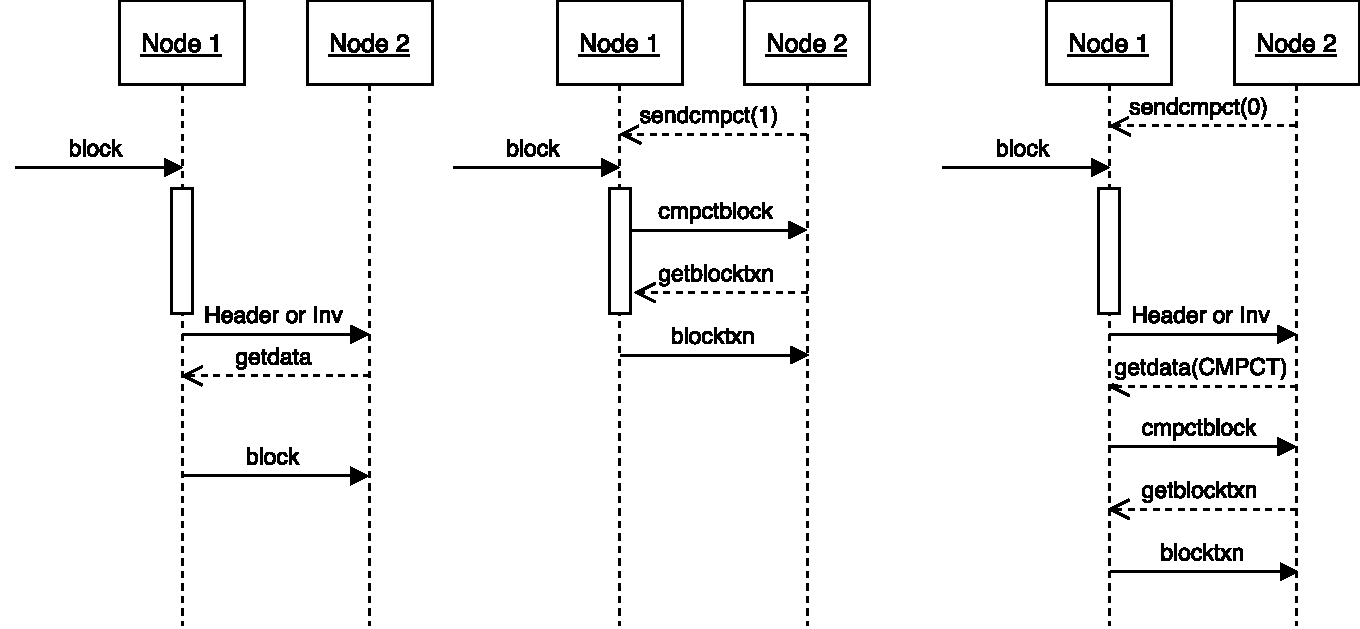
\includegraphics[scale=0.45]{image/btc-protocol-flow.pdf}
\caption{Different relaying modes in  Bitcoin}
\label{fig:protocol-flow}
\end{figure}
\end{comment}

\paragraphe{Full Block Propagation:} The sender node first validate the block completely, then it advertise the possession of block by \code{inv} message. The receiving peer which doesn't have the block, asks for it by sending \code{getdata} message. Finally, the sender node send the block via \code{block} message. Sending full block in the network is wasting network bandwidth since we are re-sending all of the transaction and nodes have some of transaction in their memory pool. The messages transmitted in this mode is: 

\code{\textbf{block:}} It consist of block version information, previous block hash, merkle root of a Merkle tree collection which is a hash of all transactions related to this block. Sending  the new block forwarded through all the network.

%\amir{the two parts are uneven regarding how much you discuss}
\paragraphe{Compact Block Propagation:}
From the middle of 2016 in \code{0.13.0} version, Bitcoin protocol start to forward blocks as compact blocks which means instead of forwarding full blocks in network, only a sketch of block is sent. The sketch include 80-byte block's header, the short transactions IDs used for matching already-available transactions and select of transactions which sending peer expect that a receiving peer may be missing.% After receiving the compact block, the receiving peer tries to reconstruct the block at its end, from the already received transactions and the one in compact block. In this way the waste of sending each transaction twice is reduced. The advantage of compact block relaying is reducing the spikes in the bandwidth and  also reduce propagation delay. The messages transmitted in this mode are: 

\code{\textbf{sendcmpct:}} This message informs the receiving peer about the mode of communication the sending peer has chosen (low or high bandwidth). %If the first byte of the message is set to 1 the sender is indicating that it wants to receive blocks as soon as possible and it is working in the high-bandwidth mode. If the first byte of the message is set 0 the sender is saying that it wants to minimize bandwidth usage as much as possible and it is working in the low-bandwidth mode.

\code{\textbf{cmpctblock}:} This message introduced in the compact block relaying and is presenting a sketch of block.

\code{\textbf{getblocktxn}:} This message is introduced in compact block relaying and is used to request for the transactions that are missed by sending a list of their indexes. 

\code{\textbf{blocktxn}:} This message is introduced in compact-block relaying and is used to provide some of the transactions in a block, as requested.

\begin{comment}
Compact block relaying works in high and low bandwidth settings. In high bandwidth the receiving peer doesn't oblige the sending peers to ask for permission first. So, multiple peers can send the compact block to receiving node. Then at last the sender node sends the missing transactions by \code{blocktxn} message. It is worth mentioning \bc works in high bandwidth mode with up to 3 peers. 
However, in low bandwidth mode, since bandwidth is its bottleneck, the receiving node oblige other nodes to ask for permission first. So, the sender first advertise the block possession by \code{inv} message. Then, the receiving node asks for the compact block by \code{getdata} and the sender will send the compact block by \code{cmpctblock} message. At last, if there is any missing transaction, the receiving node will ask for it by \code{getblocktxn} and the sender will send those transactions via \code{blocktxn}. 
\end{comment}
\begin{comment}


\begin{table*}[!h]
\caption{The list of Bitcoin communication messages}\label{tab:bc-proto-list}
\centering
\begin{tabular}{| c | l |} \hline
Message & Description \\ \hline
\code{version}
& \shortstack{Advertise the node's version. No further communication is possible until \\both peers have exchanged their version.}  \\ \hline
\code{verack}
& Reply to the \code{version} message. \\ \hline
\code{addr}
& Send information about the known nodes of the network. \\ \hline
\code{inv}
& \shortstack{Sent to advertise the knowledge of the peer about the known objects. It can be received unsolicited, \\or in reply to \code{getblocks}.} \\ \hline
\code{getdata}
& Sent in response to the \code{inv} message to retrieve information about the content of an object. \\ \hline
\code{notfound} & If the receiver of \code{getdata} cannot return the requested information, it respond with \code{notfound} \\ \hline
\code{getblocks} & It return an \code{inv} message with the list of block after the specified block in \code{getblocks} request \\ \hline
\code{getheaders} & It return a \code{headers} message with the list of block after the specified block in \code{getblocks} request \\ \hline
\code{tx} 
& Sent to describes a Bitcoin transaction in response to a 
\code{getdata} message. \\  \hline
\code{block} &  \code{block} message is sent in response to a \code{getdata} message \\ \hline
\code{headers} &  Return a list of block headers, in respond to \code{getheaders} \\ \hline
\code{getaddr} & A node sends \code{getaddr} to ask about the known peer  from other peers  \\ \hline
\code{mempool} & It asks about the transaction in mempool of other peers \\ \hline
\code{ping}
& Show the TCP/IP connection is still valid. \\ \hline
\code{pong}
& Response to \code{ping} message. \\ \hline
\code{reject} & It show a message has been rejected \\ \hline
\code{sendheaders} & let other peers to send headers without \code{inv} message \\ \hline
\code{sendcmpct} &  let other peers to send compact blocks   \\ \hline
\code{cmpctblock} & it used in stead of \code{block}, to send cmpctblock \\ \hline
\code{getblocktxn} & it indicate missing block in compact block transaction \\ \hline
\code{blocktxn} & To send missing block in compact block transaction \\ \hline
\end{tabular}
\label{table:msg_description}
\end{table*}
\end{comment}


\begin{comment}
\section{Distribution of Packet Sizes over Tor}\label{sec:bcshape}

Figure~\ref{fig:tor_reg_traffic_pkt_size_upstream}-\ref{fig:tor_fullblock_pkt_size_downstream} shows the upstream and downstream packet distribution of HTTP and \bc traffic behind Tor.
\begin{figure}[t]
\begin{subfigure}{0.48\linewidth}
\centering
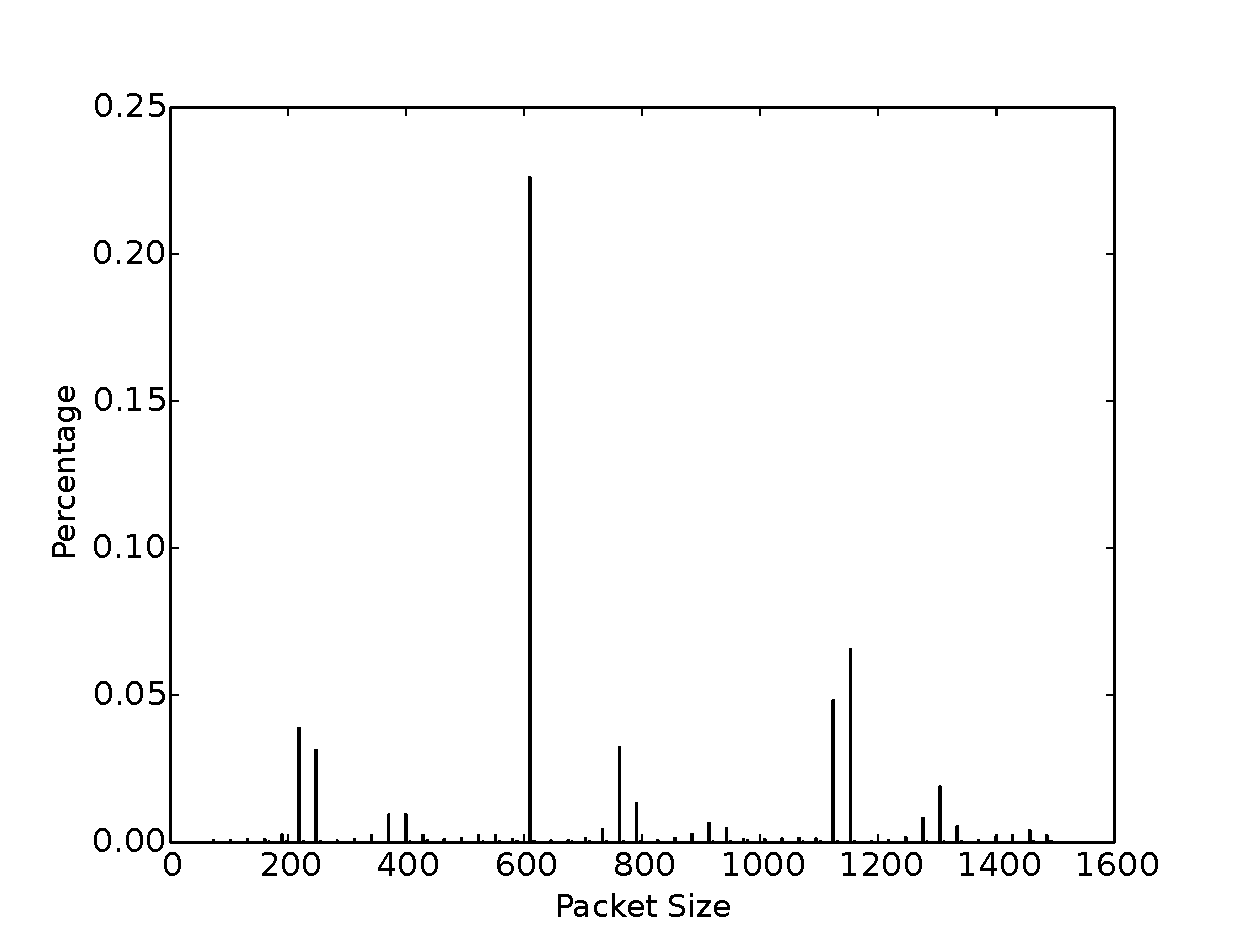
\includegraphics[width=\linewidth]{image/tor_reg_traffic_pkt_size_upstream.eps}
\caption{HTTP, upstream}
\label{fig:tor_reg_traffic_pkt_size_upstream}
\end{subfigure}
\begin{subfigure}{0.48\linewidth}
\centering
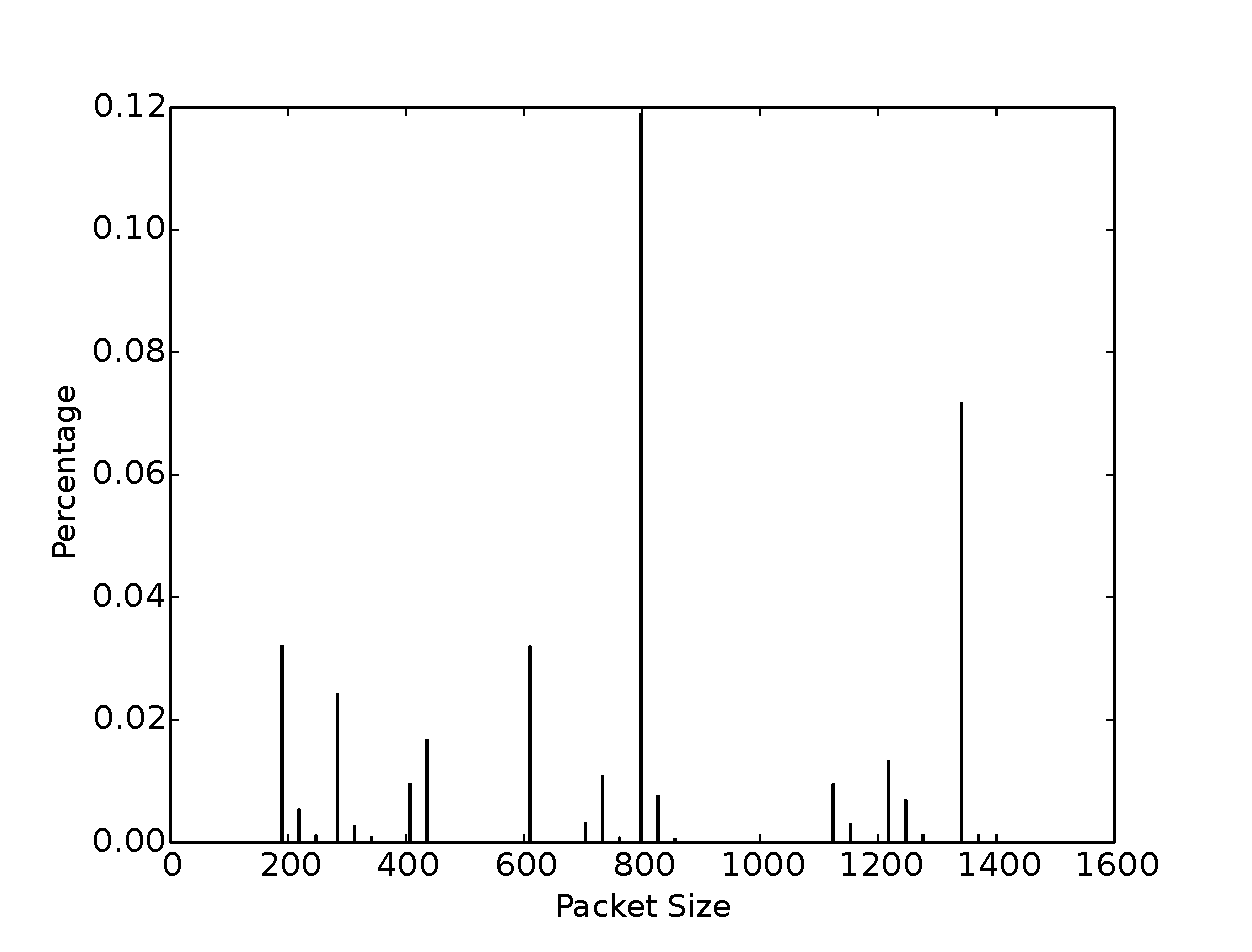
\includegraphics[width=\linewidth]{image/tor_reg_traffic_pkt_size_downstream.eps}
\caption{HTTP, downstream}
\label{fig:tor_reg_traffic_pkt_size_downstream}
\end{subfigure} 
\begin{subfigure}{0.48\linewidth}
\centering
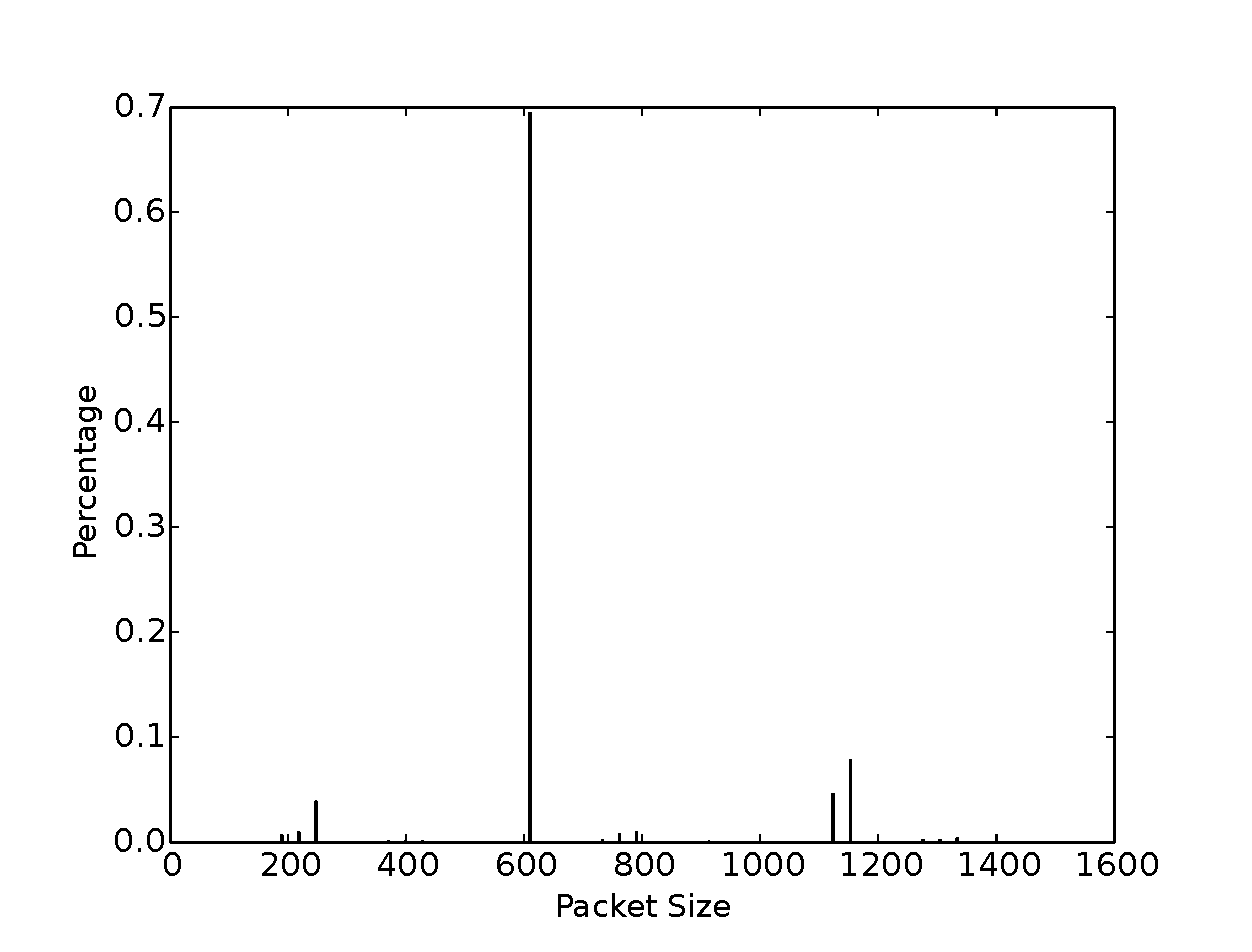
\includegraphics[width=\linewidth]{image/tor_compact_block_pkt_size_upstream.eps}
\caption{Bitcoin, Compact block, upstream}
\label{fig:tor_compact_block_pkt_size_upstream}
\end{subfigure}
\begin{subfigure}{0.48\linewidth}
\centering
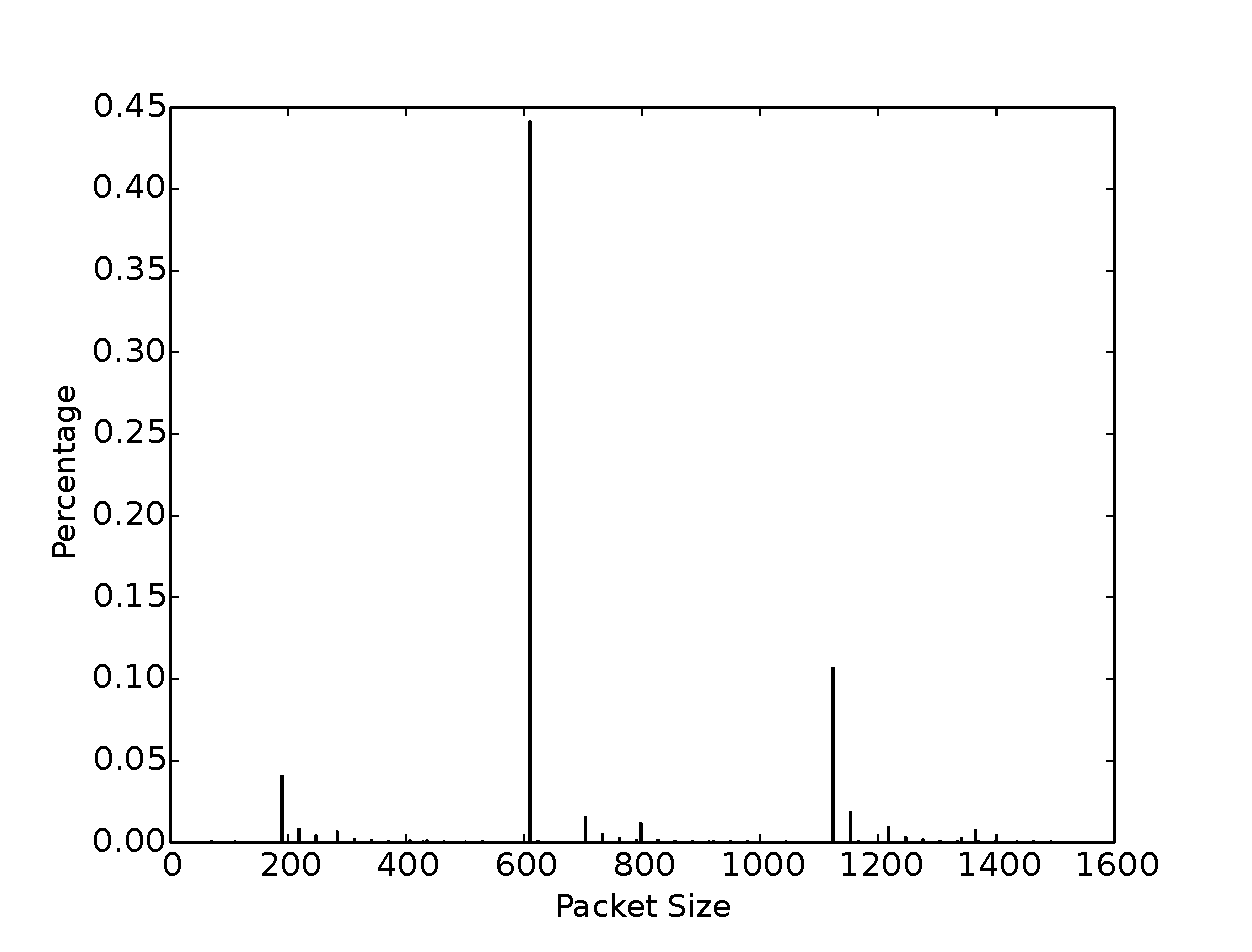
\includegraphics[width=\linewidth]{image/tor_compact_block_pkt_size_downstream.eps}
\caption{Bitcoin, Compact block, downstream}
\label{fig:tor_compact_block_pkt_size_downstream}
\end{subfigure} 
\begin{subfigure}{0.48\linewidth}
\centering
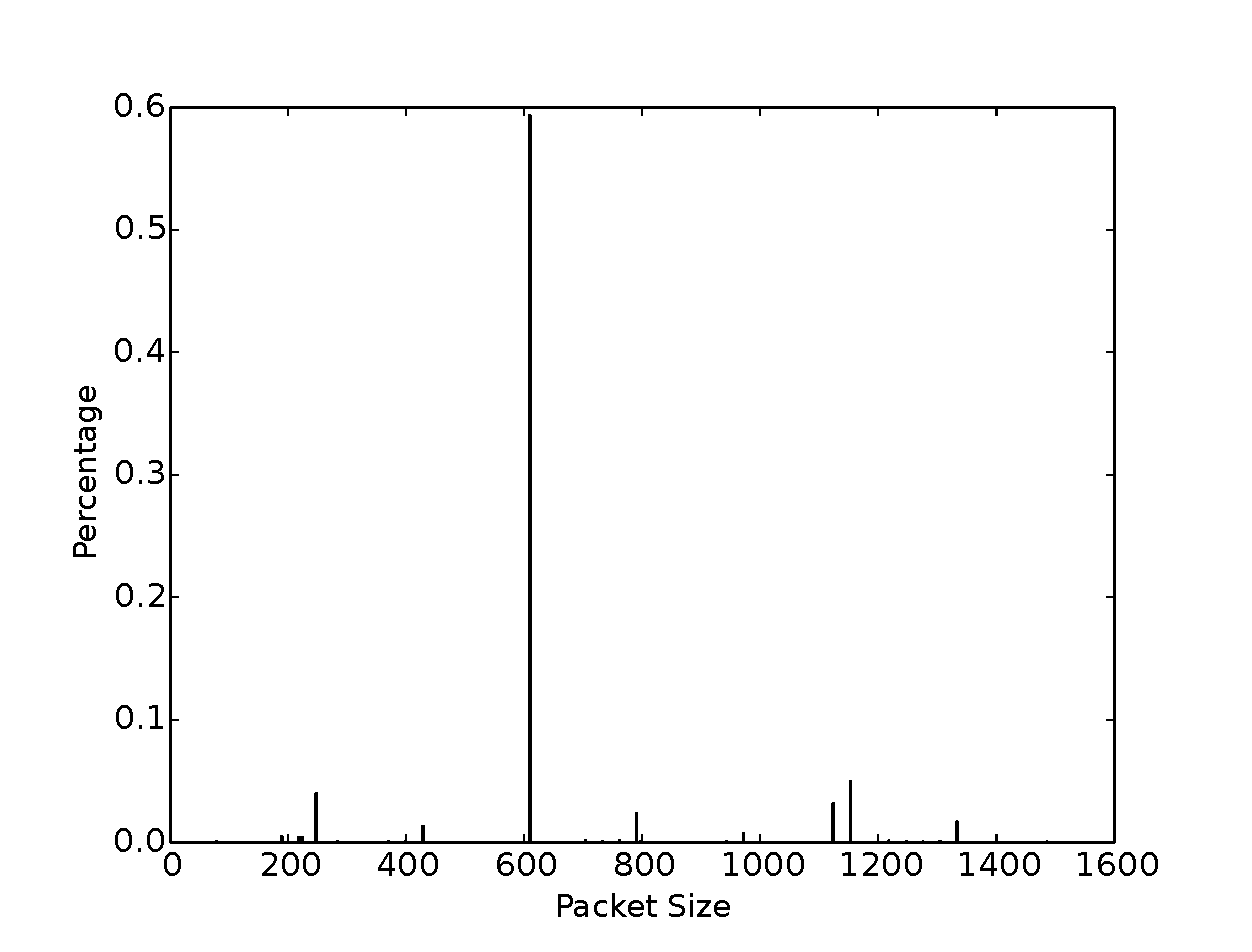
\includegraphics[width=\linewidth]{image/tor_fullblock_pkt_size_upstream.eps}
\caption{Bitcoin, Full block, upstream}
\label{fig:tor_fullblock_pkt_size_upstream}
\end{subfigure}
\begin{subfigure}{0.48\linewidth}
\centering
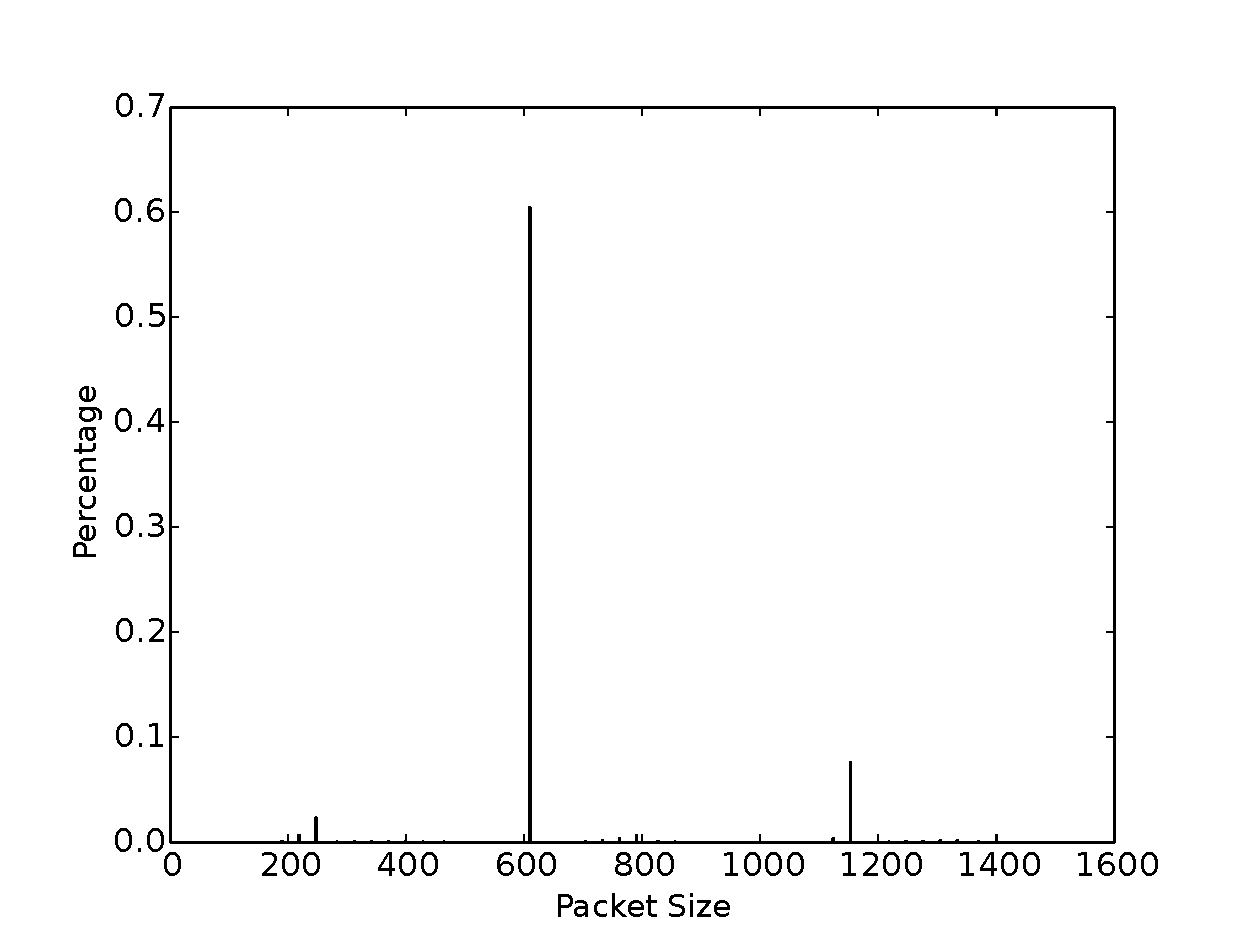
\includegraphics[width=\linewidth]{image/tor_fullblock_pkt_size_downstream.eps}
\caption{Bitcoin, Full block, downstream}
\label{fig:tor_fullblock_pkt_size_downstream}
\end{subfigure}
\caption{Distribution of packet sizes of HTTP and Bitcoin traffic behind Tor}
\end{figure}
\end{comment}
%\section{Algorithm for Window-based classifier}

\section{Threat Model}



\fatemeh{we did not have any text in  here}
\red{this section is so bad. it is not about threat model and it is too short. please put back the previous text that we had so i edit. }


 





\section{Characterizing \bc Traffic}\label{sec:charachterzing_bc}
%\red{why this section has only one subsection? what happened to the rest of the section? you seem to have randomly deleted text to fit in the page limit. please put back whatever we had. you need to shrink not delete sections}

%\fatemeh{I did not remove the text randomly. I removed the ones that was not needed and did not add anything to the context (In my opinion)}
%\par In this section, we investigate the characteristic of Bitcoin traffic, try to identify Bitcoin traffic in unencrypted and encrypted traffics. First we analyze the block propagation delay in Bitcoin network. Then, we use the results to come up with a scheme to correlate the client's traffic with a known baseline for Bitcoin blockchains in order to detect the Bitcoin usage in client traffic.


%All of our experiments in this section follow the 
 %experimental setup and datasets described in Section~\ref{sec:exp-dataset}. 
\begin{comment}
\begin{table*}
\caption{Number and percentage of each message in a 31 days Bitcoin traffic in compact block relaying}
\centering
\begin{tabular}{|c|c|c|c|} \hline
Message & Packets per minute & Proportion  & Average packet size\\ \hline
\code{inv} & 173.17 & 27.240\% & 791.87\\ \hline
\code{getdata} & 13.16 & 2.070\%  & 700.33\\ \hline
\code{block} & 0.94 & 0.330 \%  & 772.74\\ \hline
\code{sendcmpct} & 1.60 & 0.253\%  & 782.88\\ \hline
\code{cmpctblock} & 2.02 & 0.319\% & 789.21 \\ \hline
\code{getblocktxn} & 0.02 & 0.003 \%  & 367.67\\ \hline
\code{blocktxn} & 0.77 & 0.121\%  & 777.16\\ \hline
\code{tx} & 277.72 & 43.688\%  & 790.00\\ \hline
\end{tabular}
\label{table:msg_proportion}
\end{table*}
\end{comment}

\begin{figure*}[h]
\centering
\begin{subfigure}{0.24\linewidth}
\centering
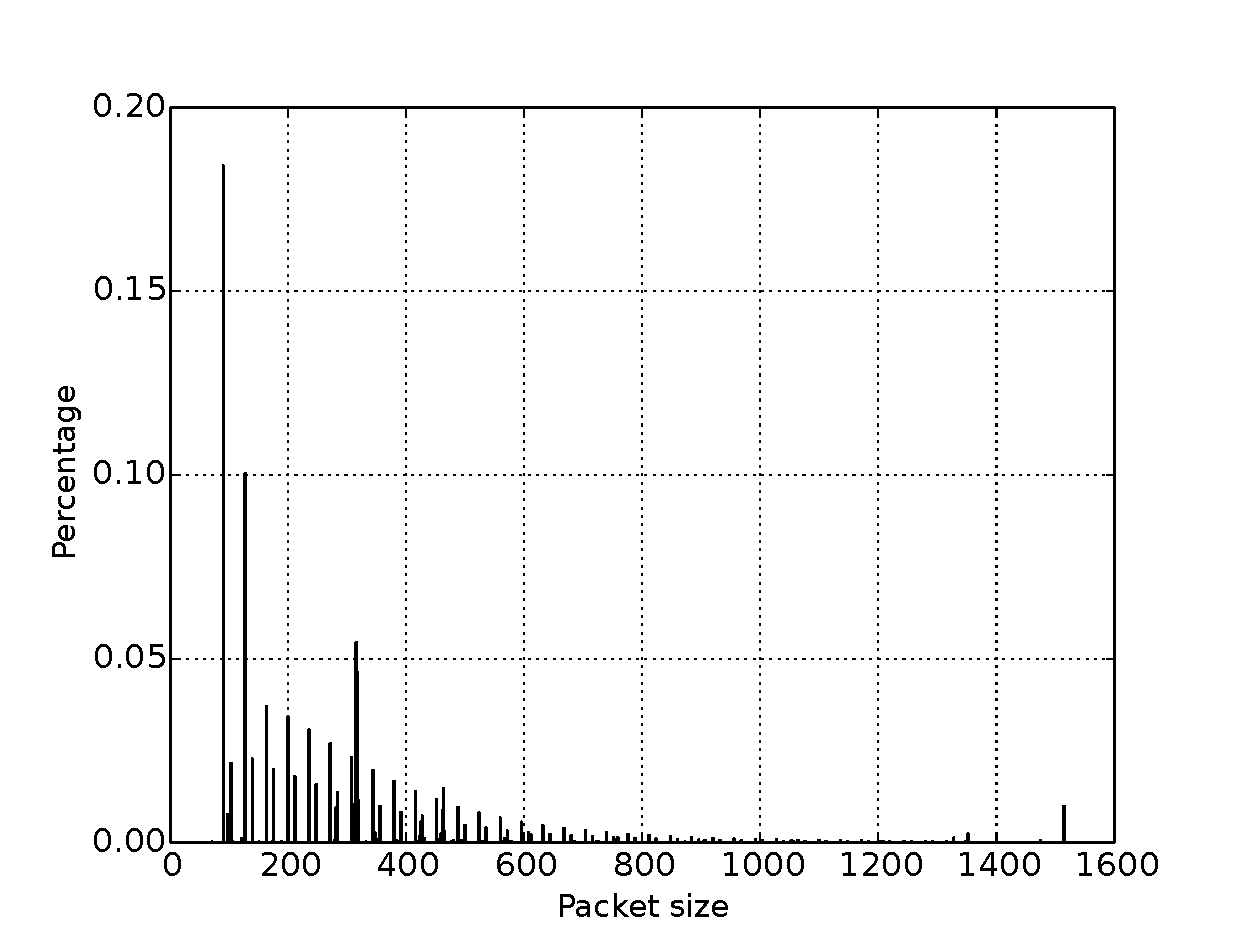
\includegraphics[width=\linewidth]{image/inv_pktsizes.eps}
\caption{\code{inv}}
\label{fig:inv_pktsizes}
\end{subfigure}
\begin{subfigure}{0.24\linewidth}
\centering
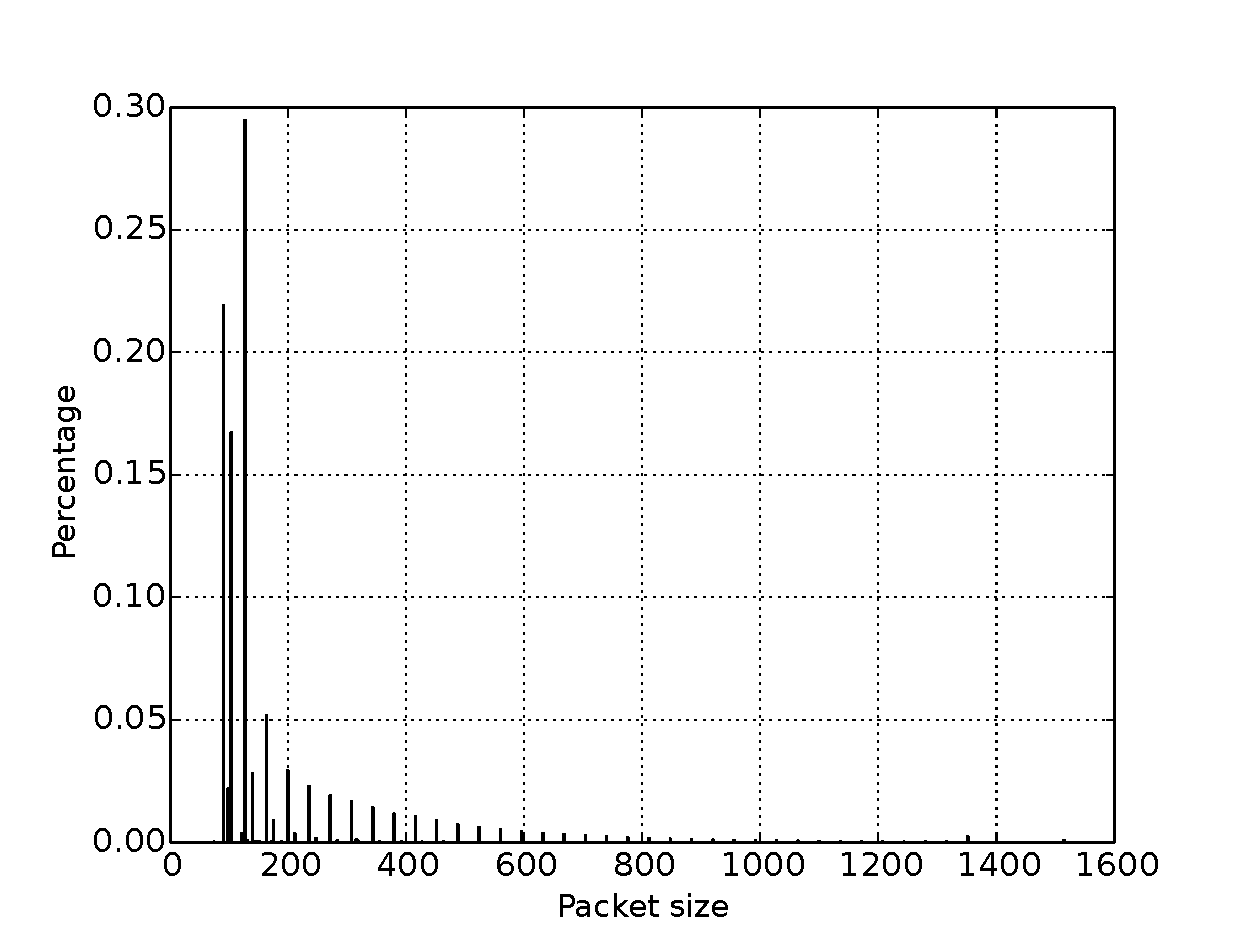
\includegraphics[width=\linewidth]{image/getdata_pktsizes.eps}
\caption{\code{getdata}}
\label{fig:getdata_pktsizes}
\end{subfigure}
\begin{subfigure}{0.24\linewidth}
\centering
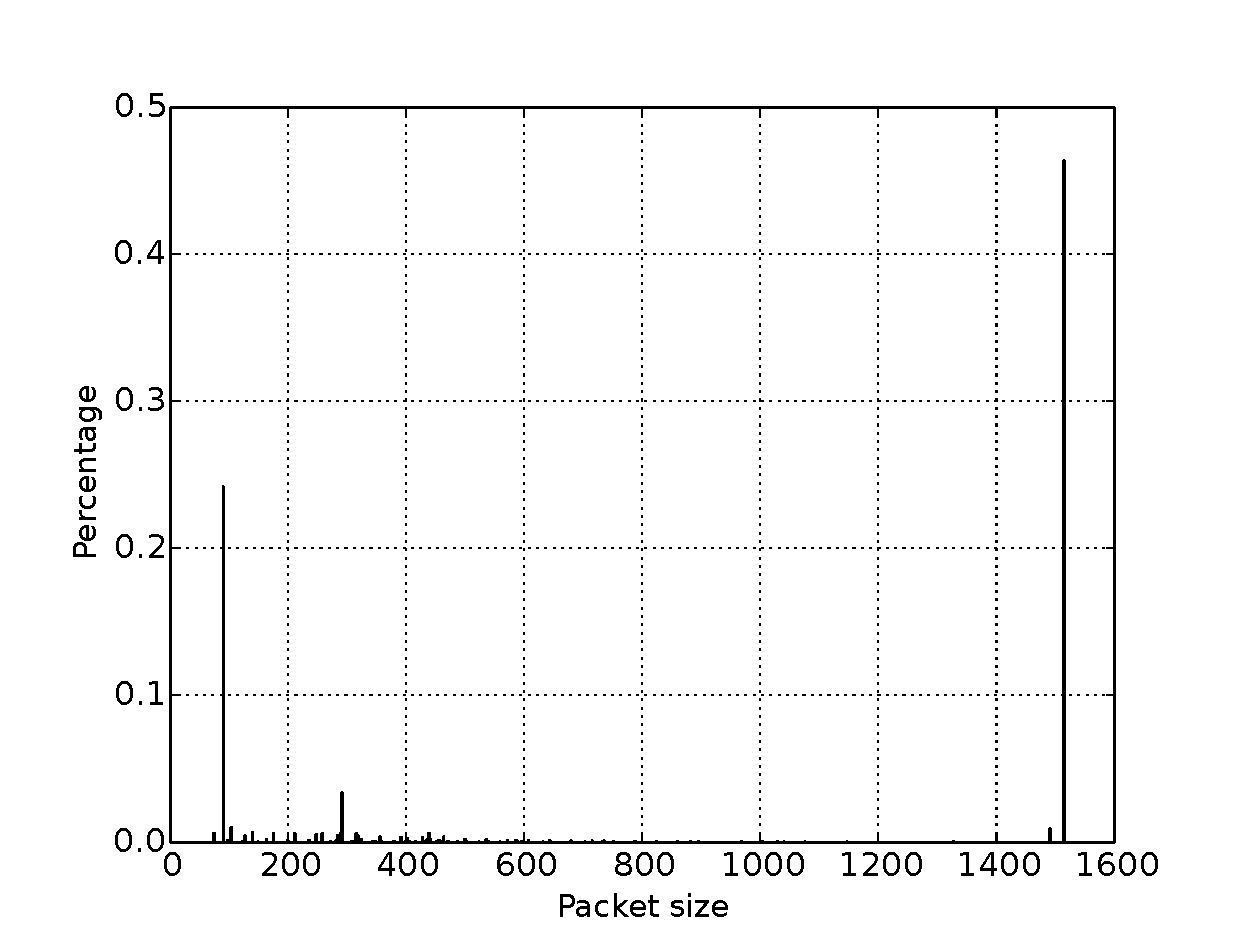
\includegraphics[width=\linewidth]{image/block_pktsizes.eps}
\caption{\code{block}}
\label{fig:block_pktsizes}
\end{subfigure}
\begin{subfigure}{0.24\linewidth}
\centering
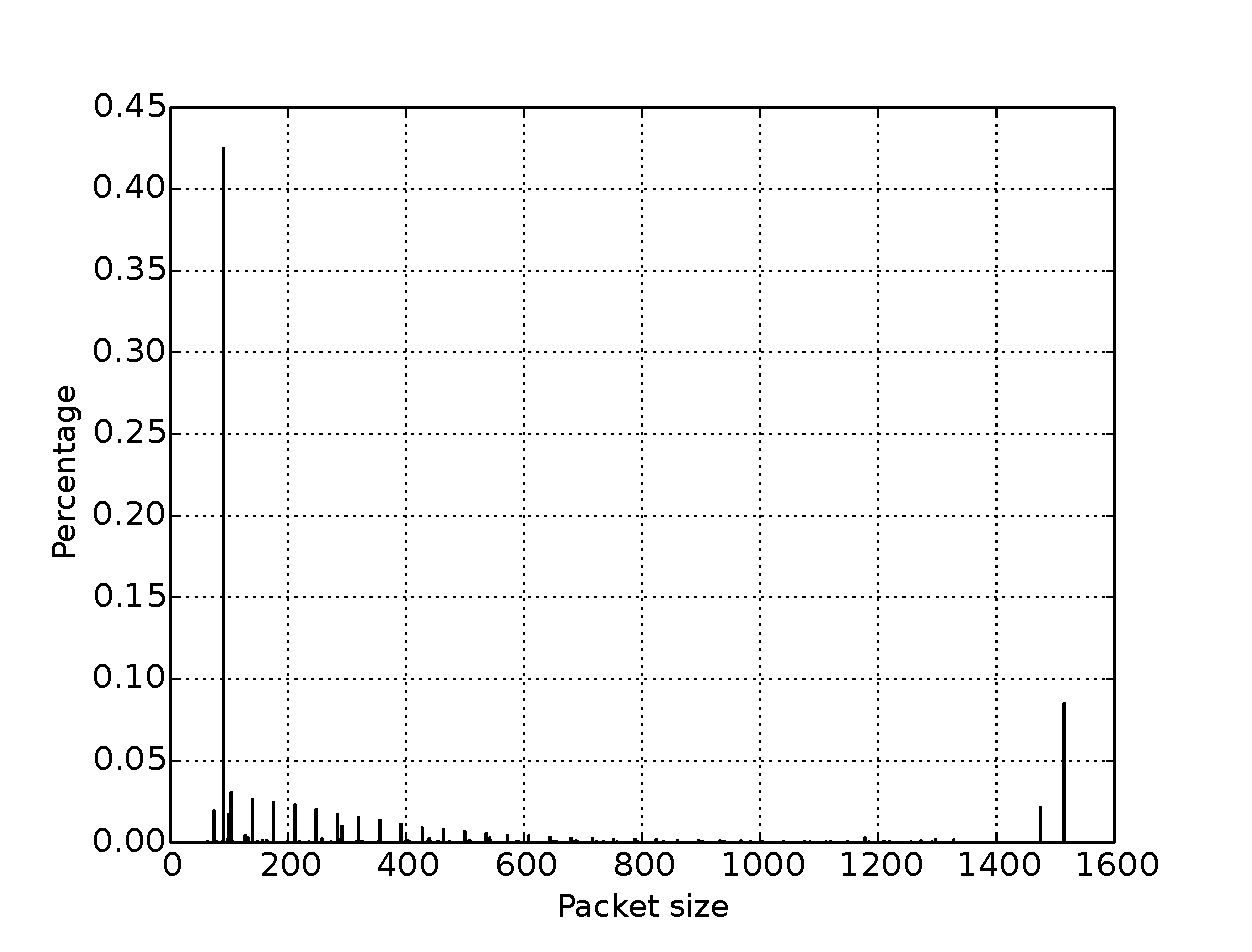
\includegraphics[width=\linewidth]{image/sendcmpct_pktsizes.eps}
\caption{\code{sendcmpct}}
\label{fig:sendcmpct_pktsizes}
\end{subfigure}
\begin{subfigure}{0.24\linewidth}
\centering
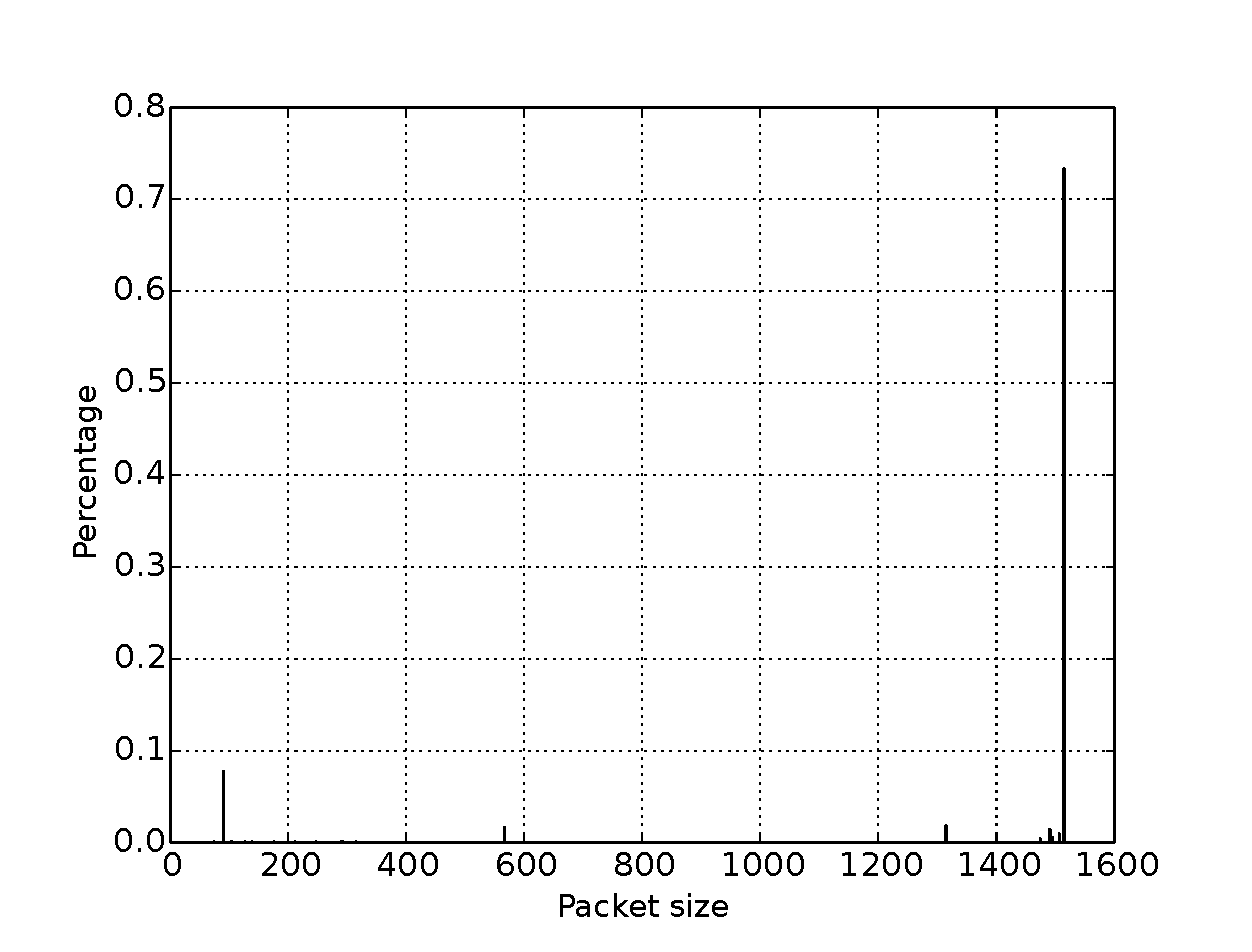
\includegraphics[width=\linewidth]{image/cmpctblock_pktsizes.eps}
\caption{\code{cmpctblock}}
\label{fig:cmpctblock_pktsizes}
\end{subfigure}
\begin{subfigure}{0.24\linewidth}
\centering
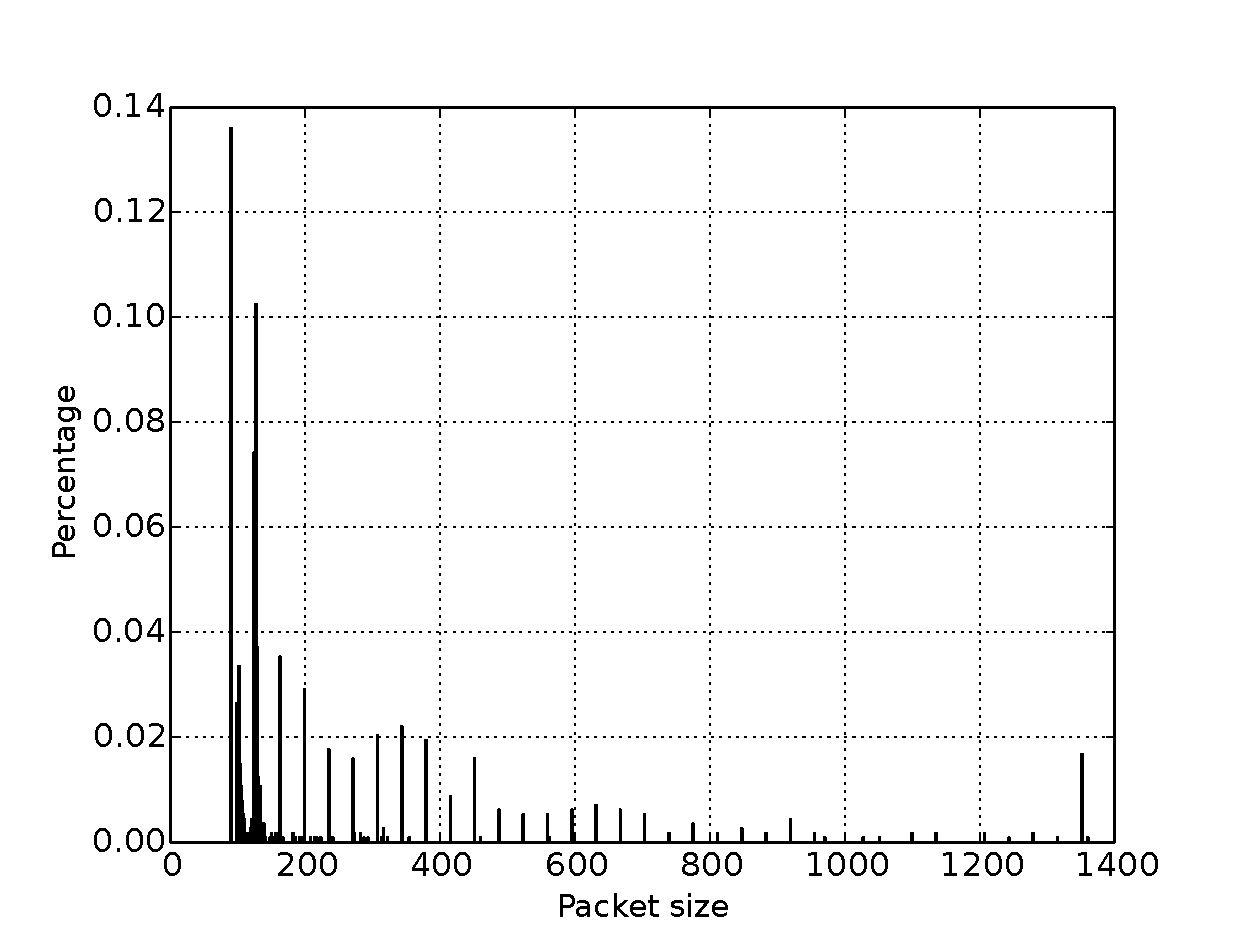
\includegraphics[width=\linewidth]{image/getblocktxn_pktsizes.eps}
\caption{\code{getblocktxn}}
\label{fig:getblocktxn_pktsizes}
\end{subfigure}
\begin{subfigure}{0.24\linewidth}
\centering
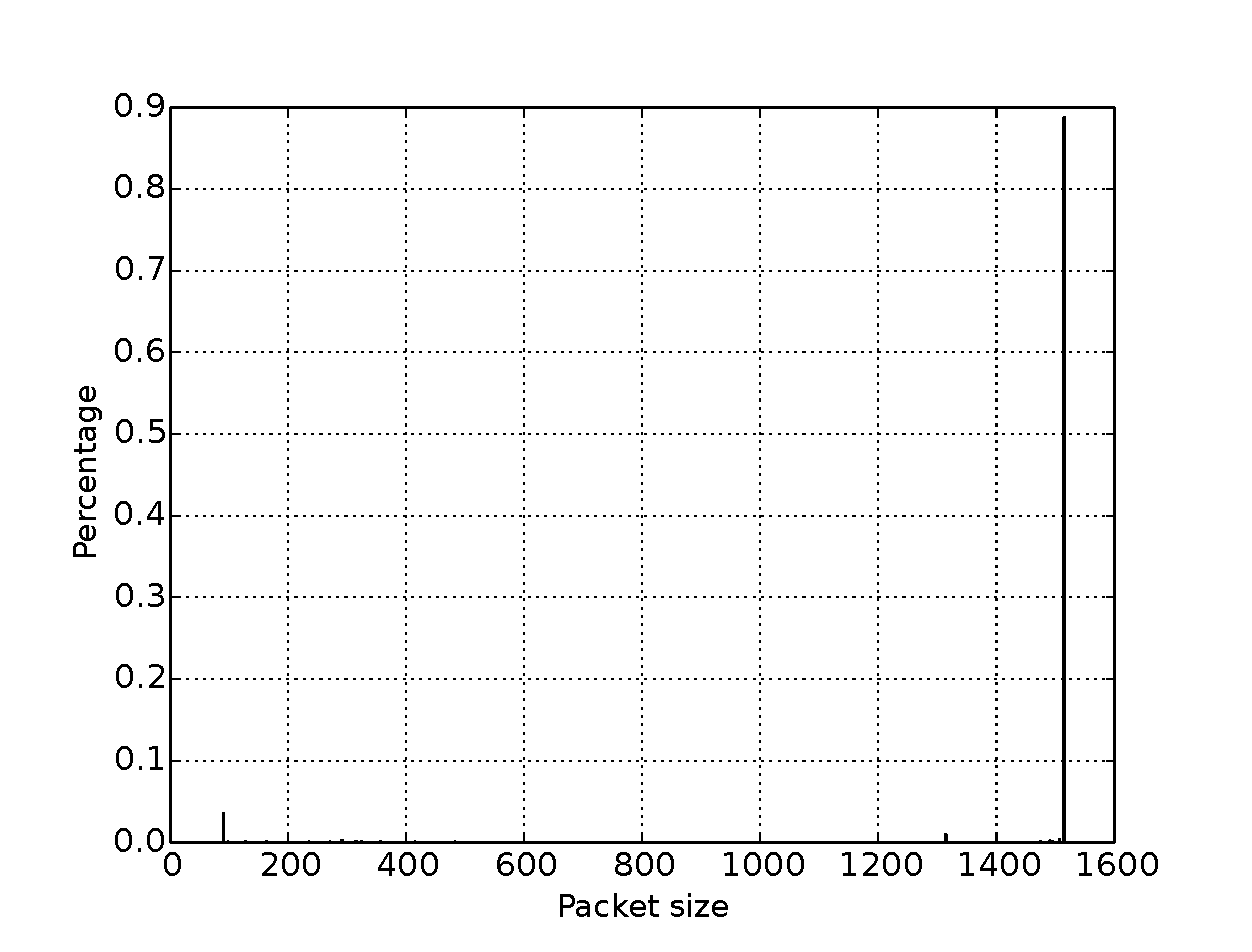
\includegraphics[width=\linewidth]{image/blocktxn_pktsizes.eps}
\caption{\code{blocktxn}}
\label{fig:blocktxn_pktsizes}
\end{subfigure}
\begin{subfigure}{0.24\linewidth}
\centering
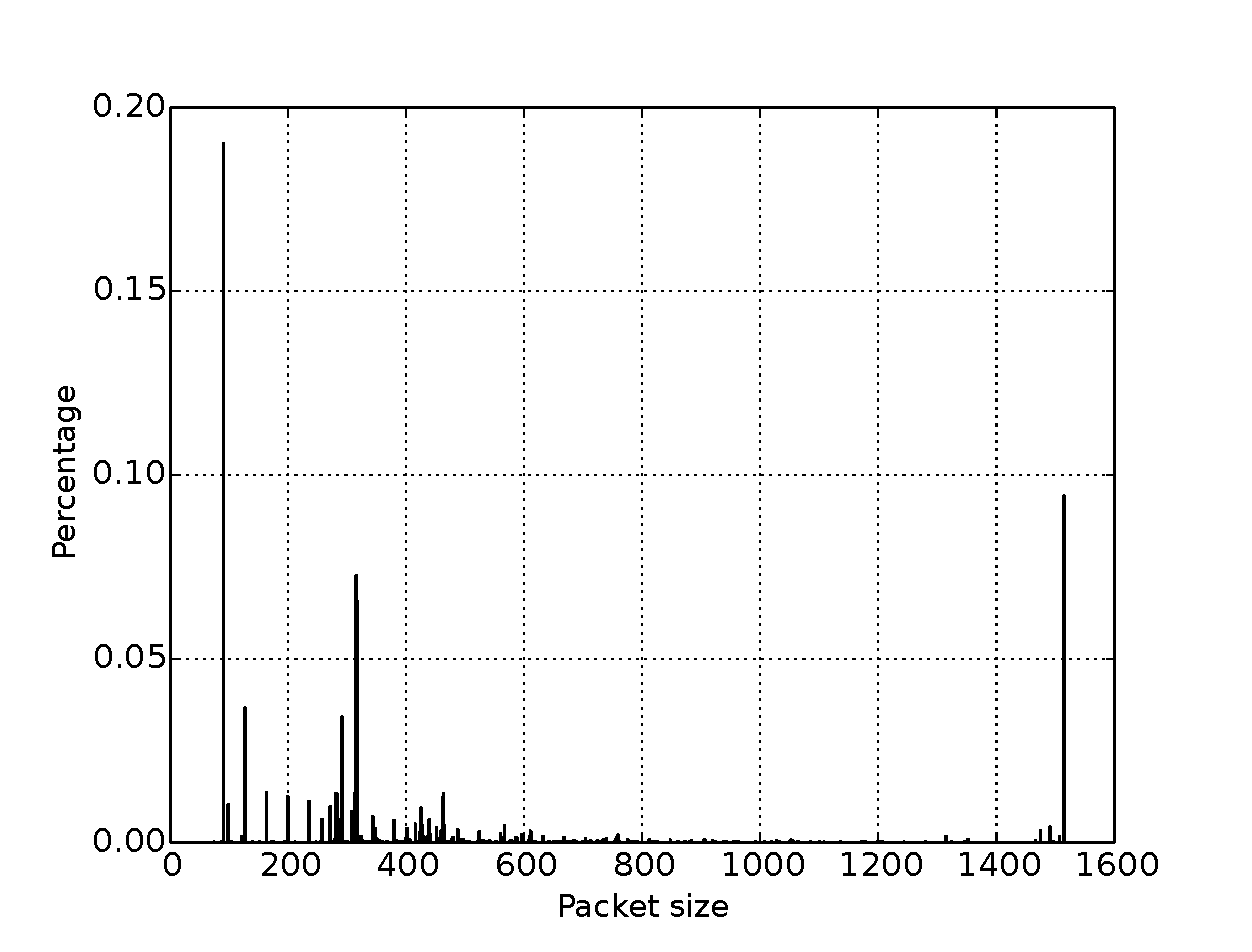
\includegraphics[width=\linewidth]{image/tx_pktsizes.eps}
\caption{\code{tx}}
\label{fig:tx_pktsizes}
\end{subfigure}
\caption{Packet size distribution of \bc communication messages in compact block relaying}\label{fig:sizedist}
\end{figure*}

%\begin{comment}
\begin{figure*}[h]
\centering
\begin{subfigure}{.24\linewidth}
\centering
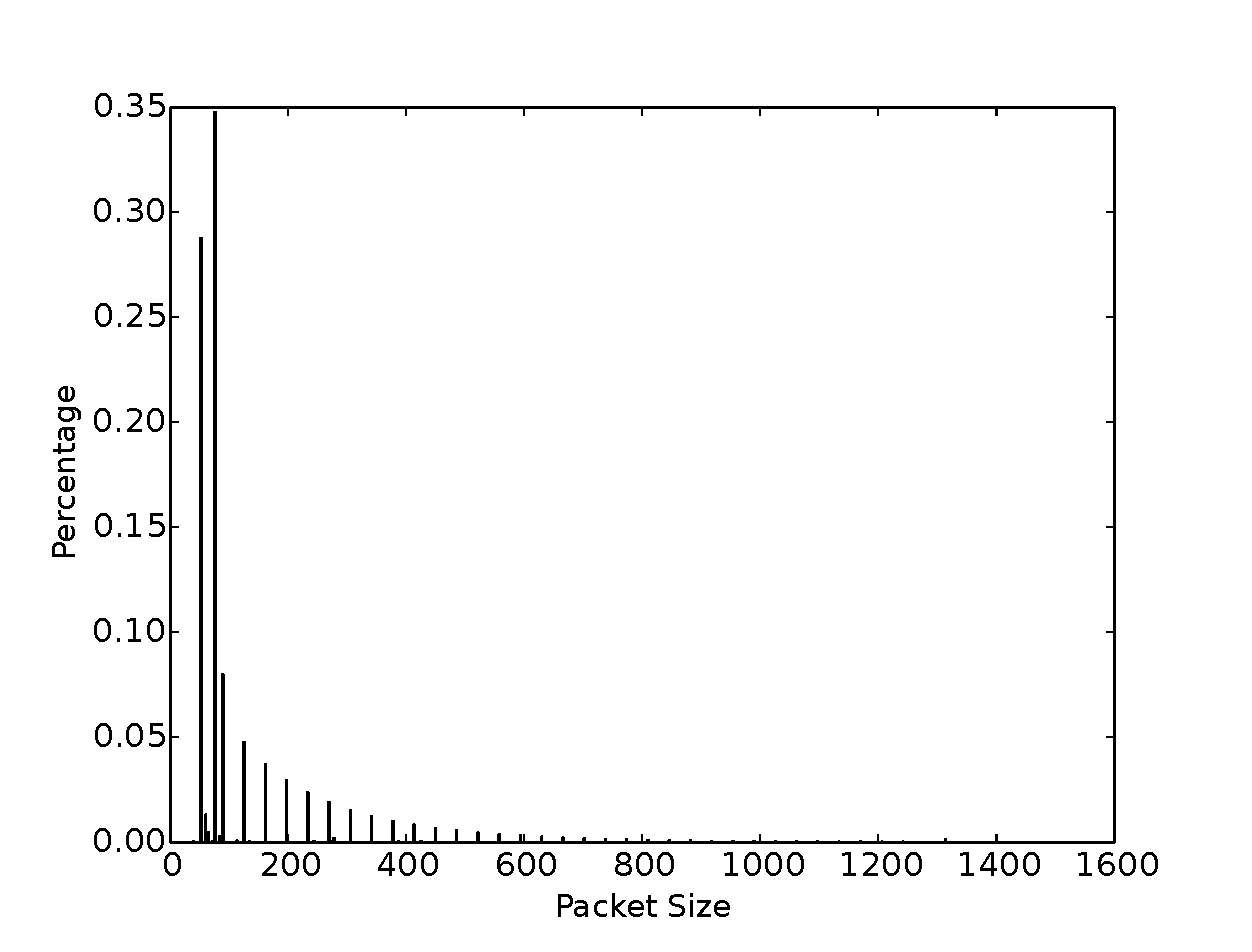
\includegraphics[width=\linewidth]{image/cmpctblock_pkt_size_upstream.eps}
\caption{Compact block, upstream}
\label{fig:aggregate_pkt_size_upstream_cmpct}
\end{subfigure}
\begin{subfigure}{.24\linewidth}
\centering
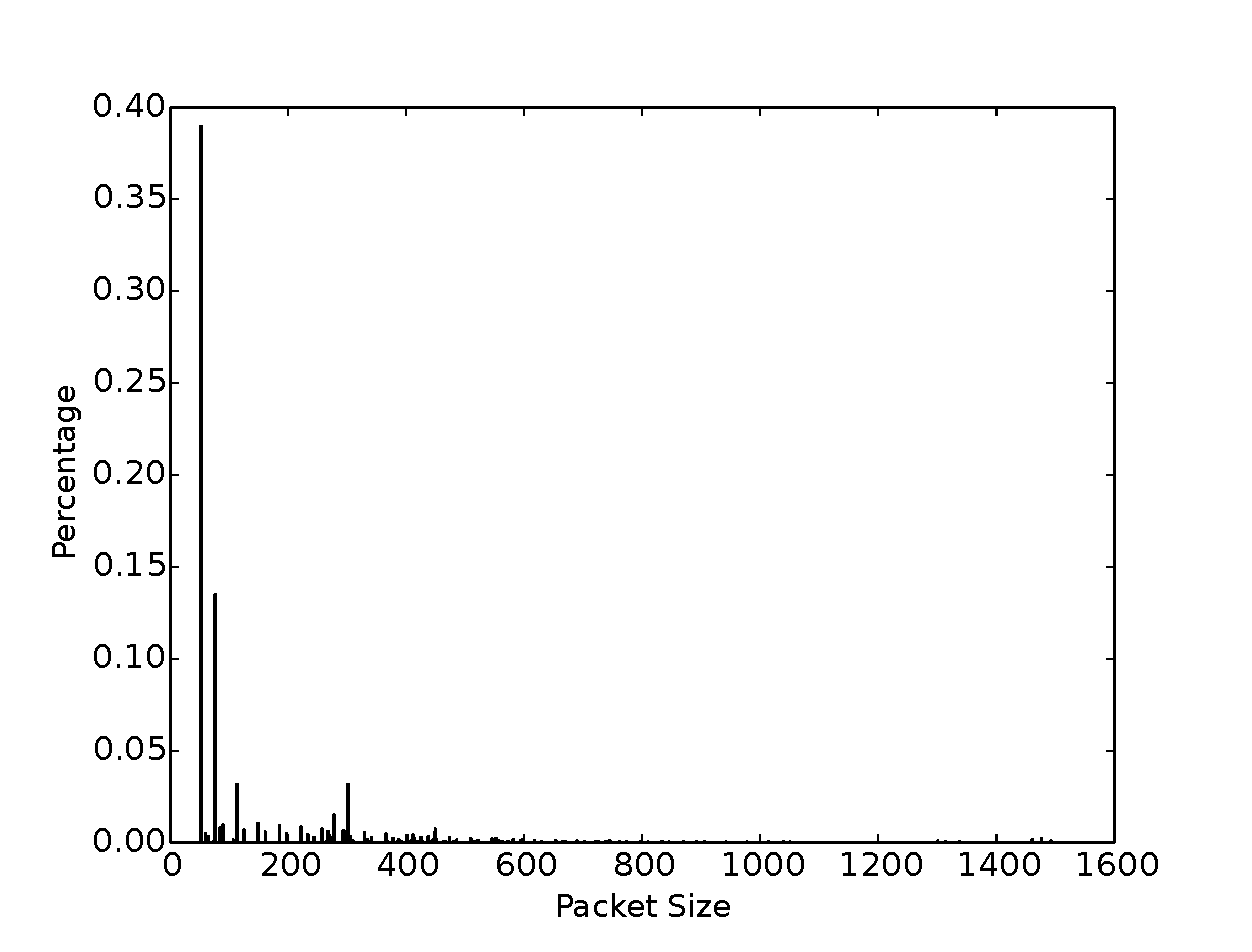
\includegraphics[width=\linewidth]{image/cmpctblock_pkt_size_downstream.eps}
\caption{Compact block, downstream}
\label{fig:aggregate_pkt_size_downstream_cmpct}
\end{subfigure}
\begin{subfigure}{.24\linewidth}
\centering
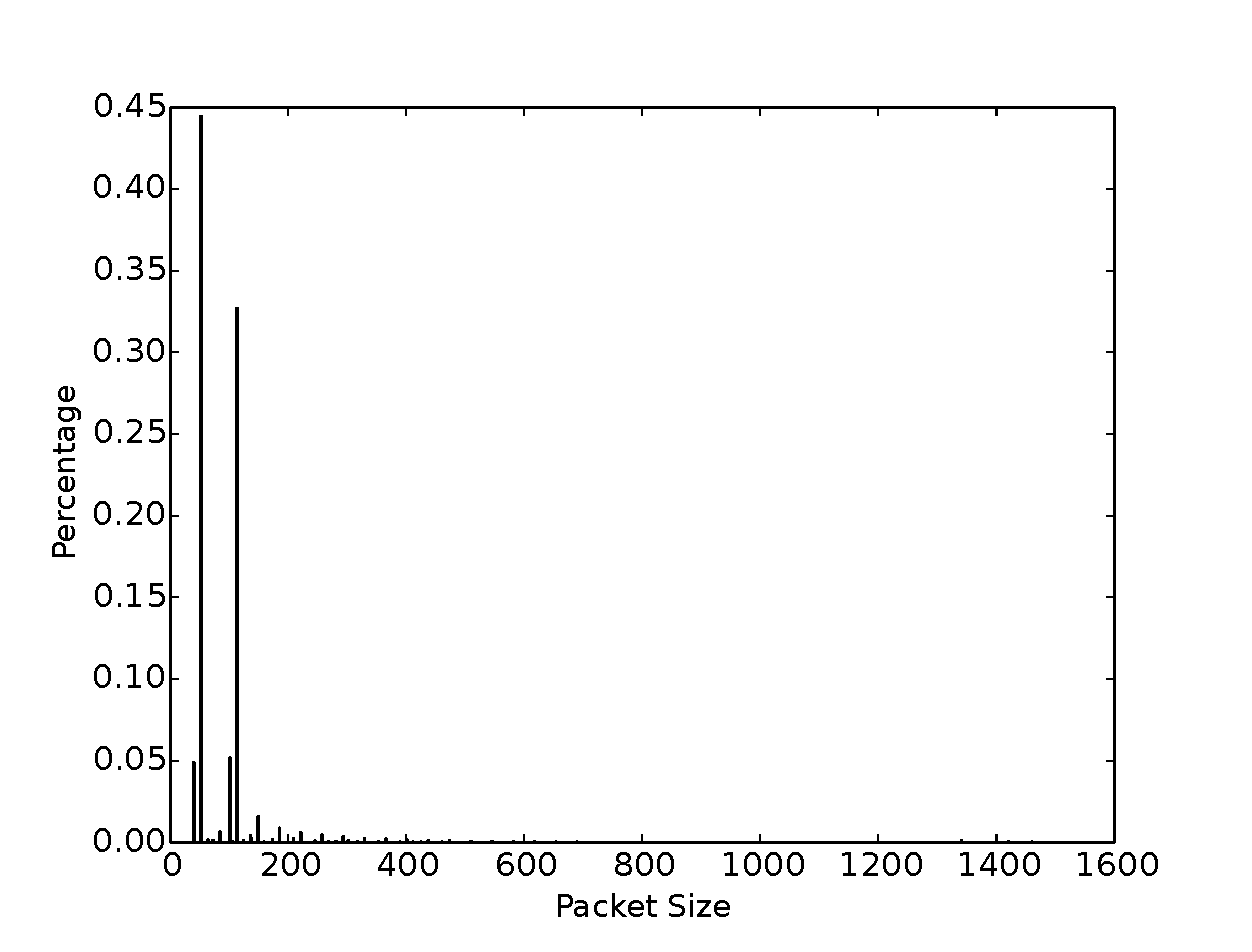
\includegraphics[width=\linewidth]{image/fullblock_pkt_size_upstream.eps}
\caption{Full Block, upstream}
\label{fig:aggregate_pkt_size_upstream_full}
\end{subfigure}
\begin{subfigure}{.24\linewidth}
\centering
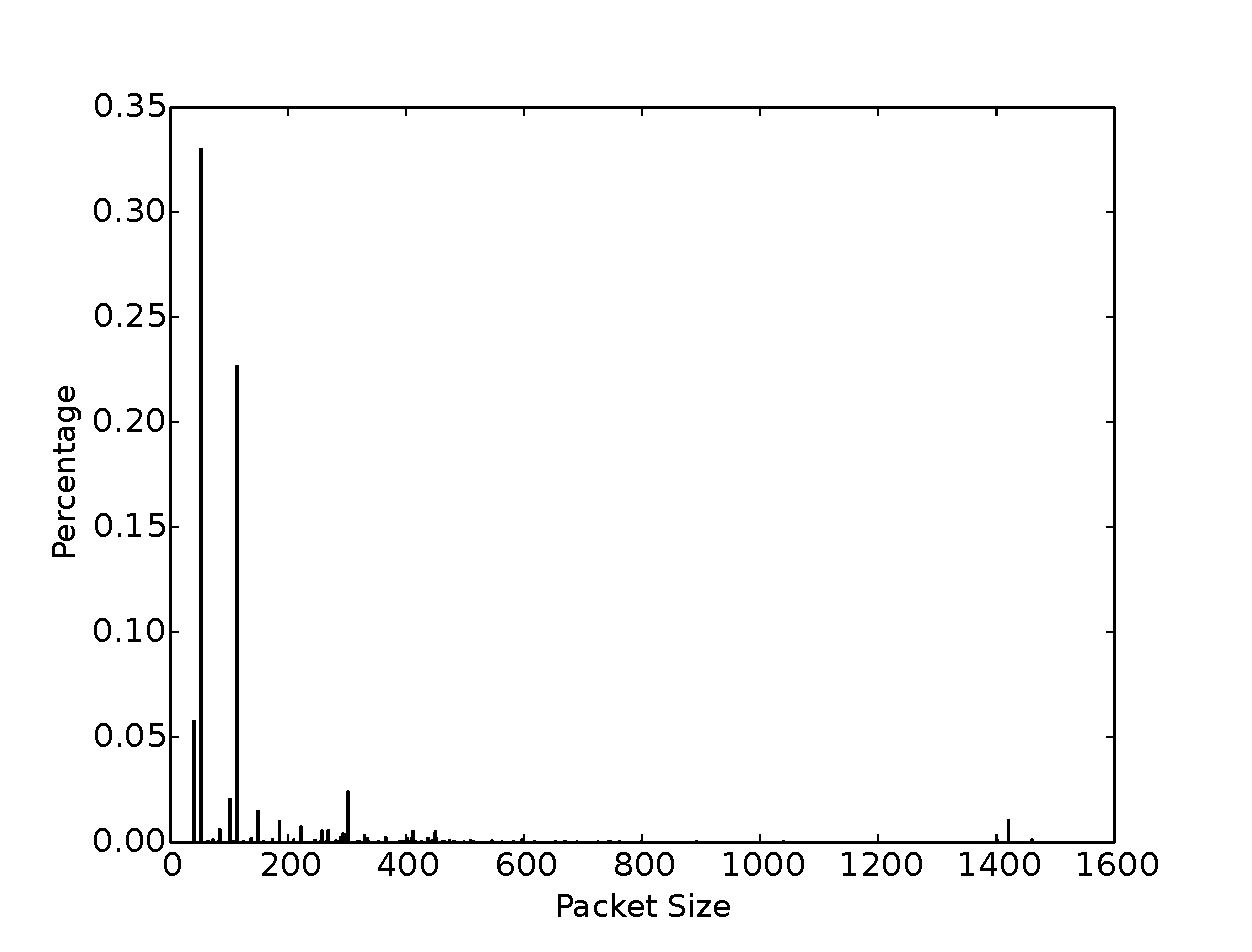
\includegraphics[width=\linewidth]{image/fullblock_pkt_size_downstream.eps}
\captionof{figure}{Full block, downstream}
\label{fig:aggregate_pkt_size_downstream_full}
\end{subfigure}
\begin{subfigure}{.24\linewidth}
\centering
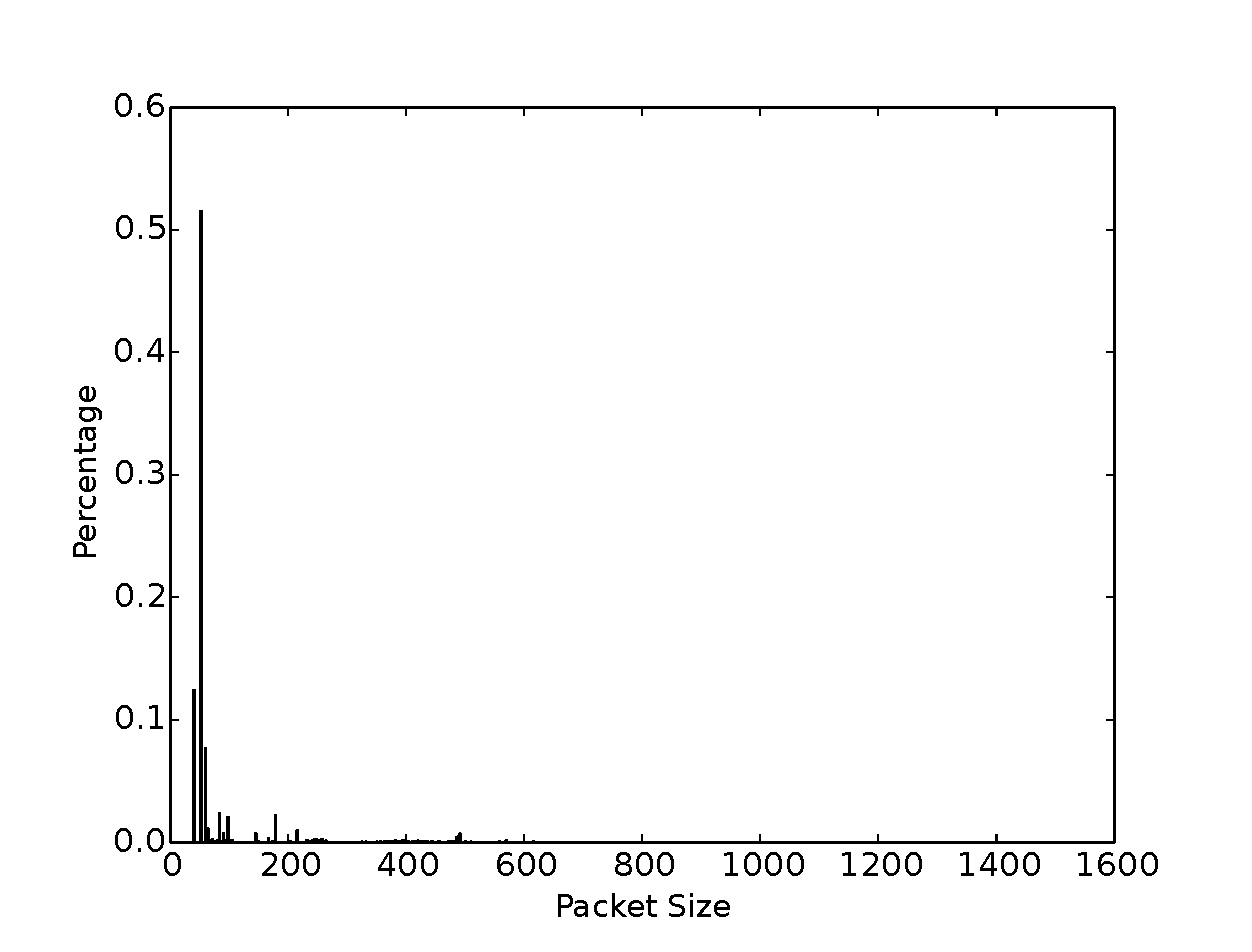
\includegraphics[width=\linewidth]{image/http_pkt_size_upstream.eps}
\caption{HTTP, upstream}
\label{fig:http_pkt_size_upstream}
\end{subfigure}
\begin{subfigure}{.24\linewidth}
\centering
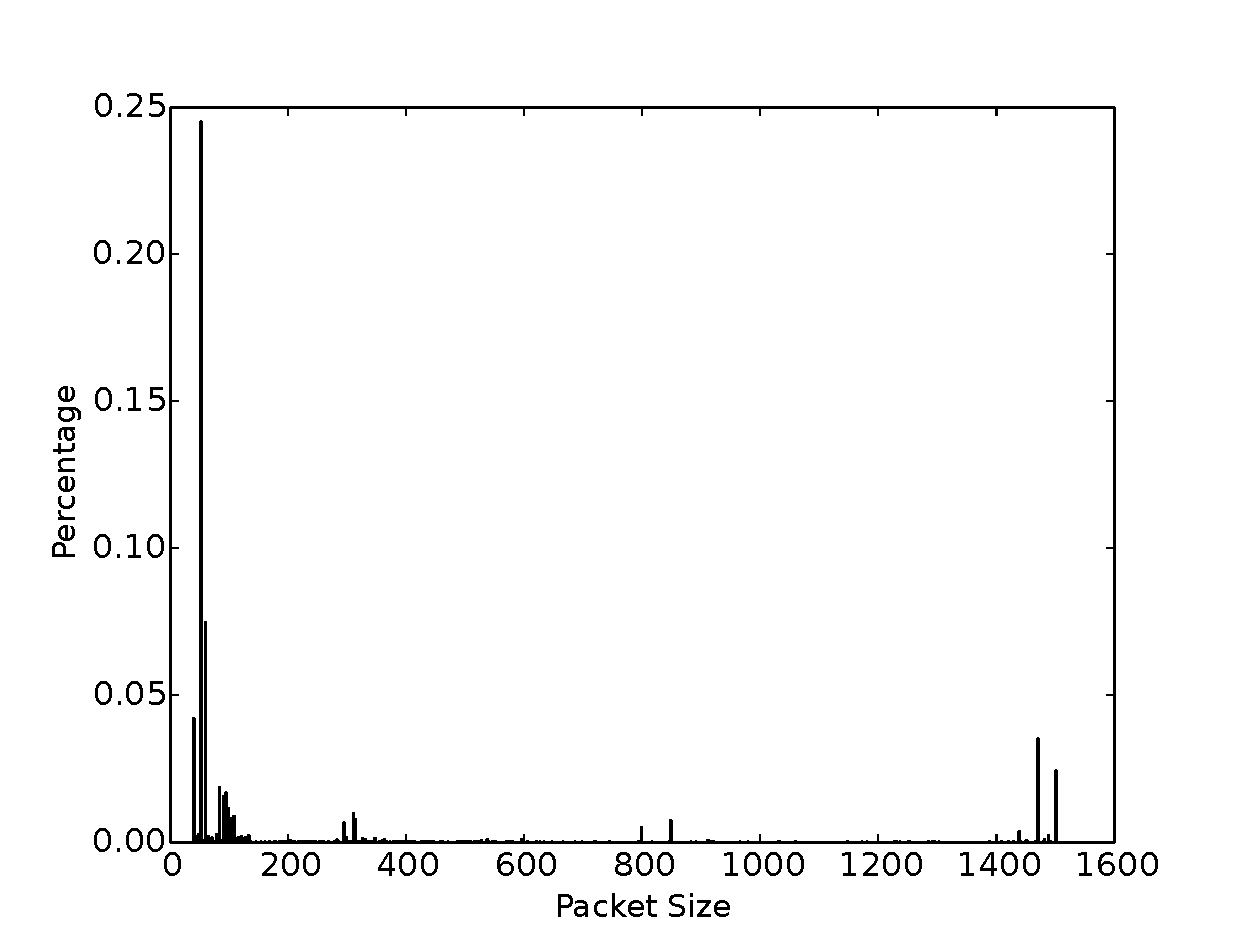
\includegraphics[width=\linewidth]{image/http_pkt_size_downstream.eps}
\caption{HTTP, downstream}
\label{fig:http_pkt_size_downstream}
\end{subfigure}
\begin{subfigure}{.24\linewidth}
\centering
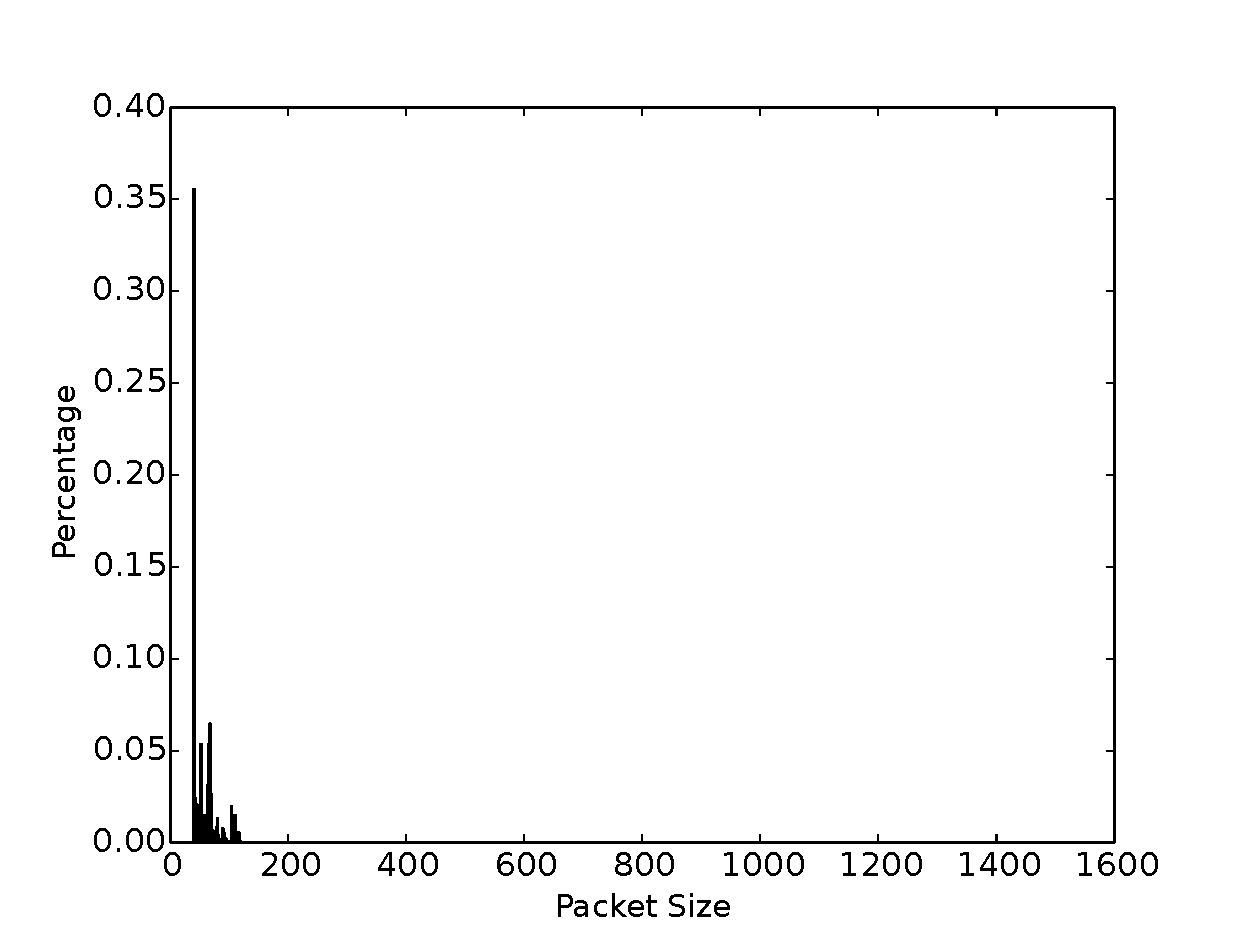
\includegraphics[width=\linewidth]{image/ftp_pkt_size_upstream.eps}
\caption{FTP, upstream}
\label{fig:ftp_pkt_size_upstream}
\end{subfigure}
\begin{subfigure}{.24\linewidth}
\centering
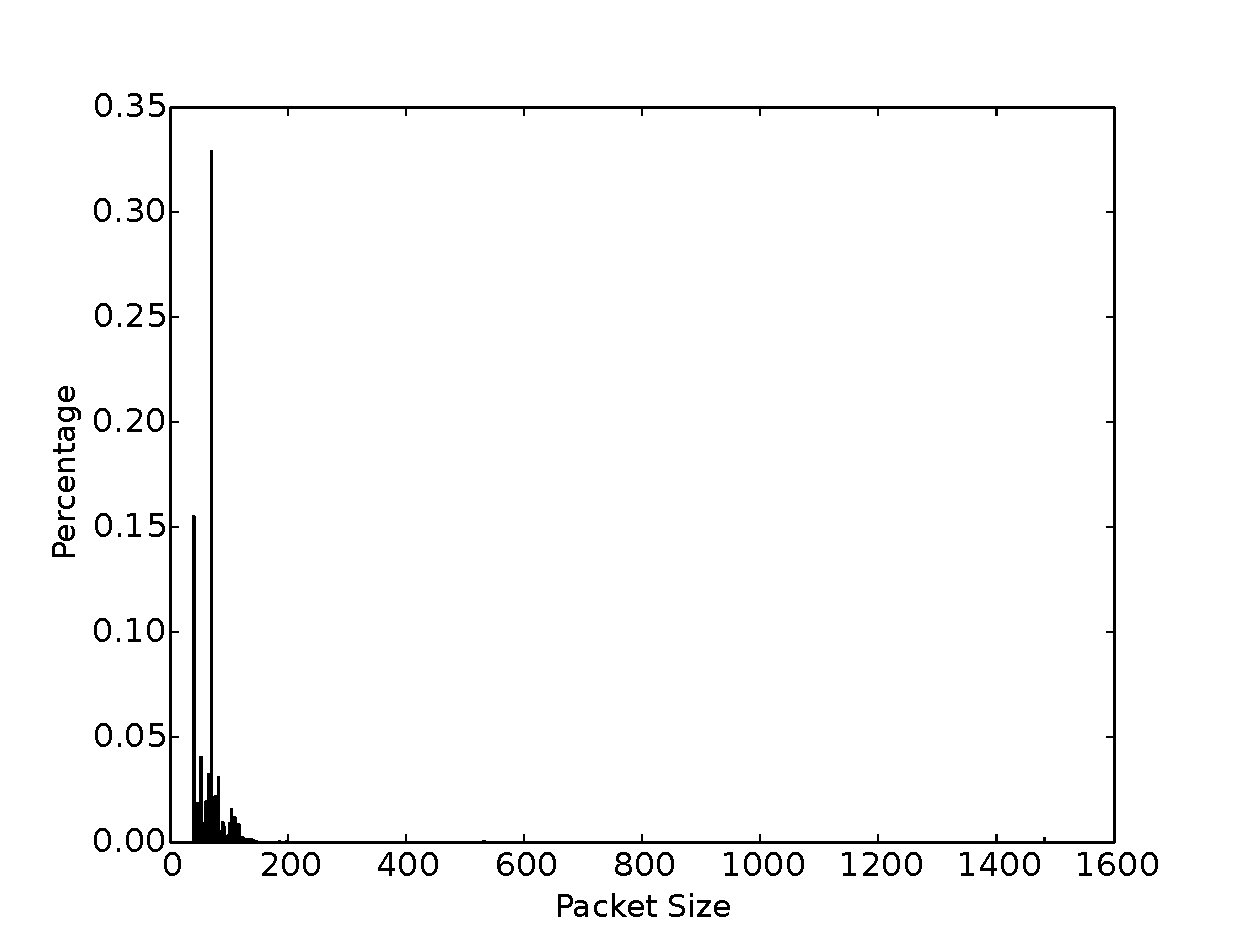
\includegraphics[width=\linewidth]{image/ftp_pkt_size_downstream.eps}
\caption{FTP, downstream}
\label{fig:ftp_pkt_size_downstream}
\end{subfigure}
\begin{subfigure}{.24\linewidth}
\centering
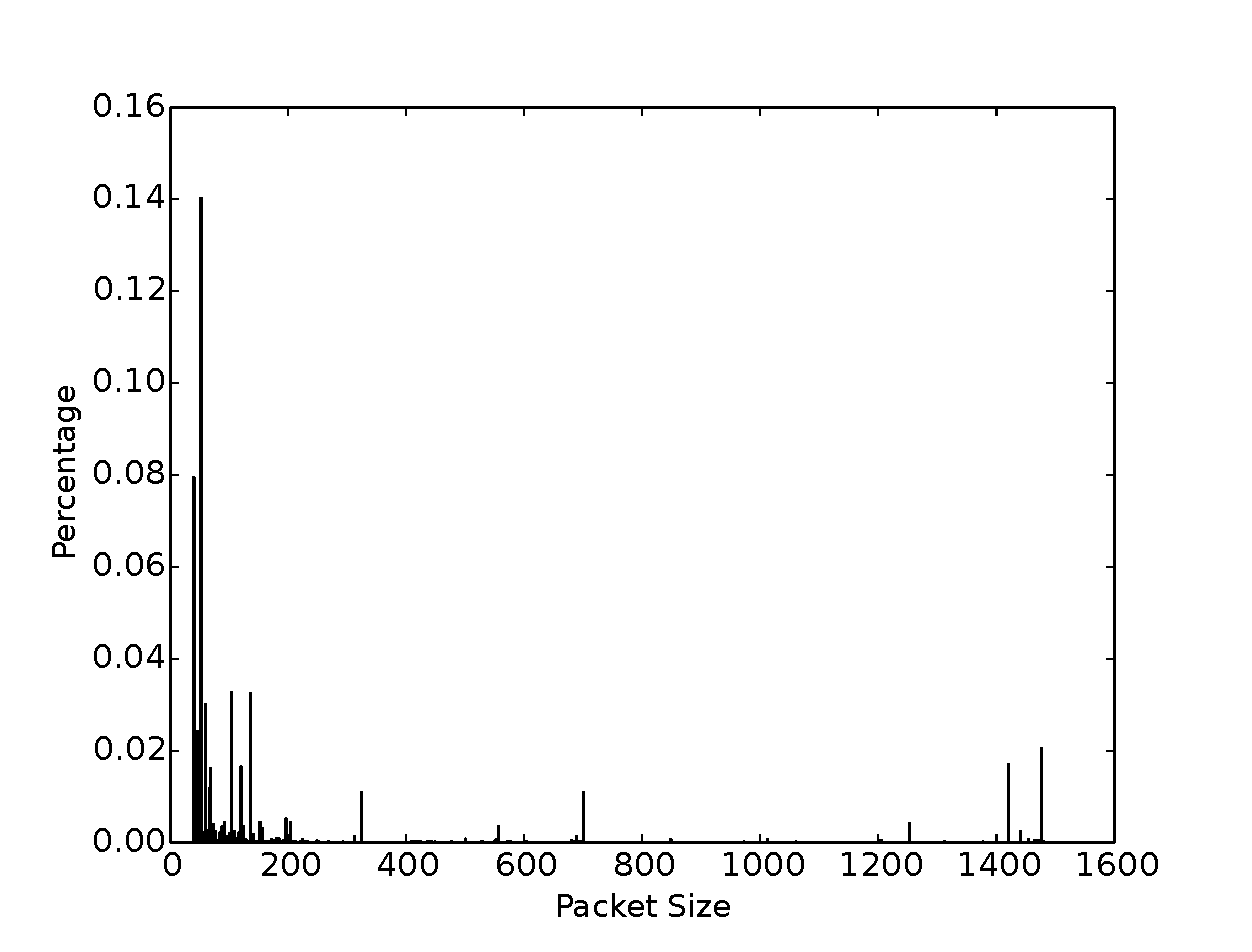
\includegraphics[width=\linewidth]{image/ssh_pkt_size_upstream.eps}
\caption{SSH, upstream}
\label{fig:ssh_pkt_size_upstream}
\end{subfigure}
\begin{subfigure}{.24\linewidth}
\centering
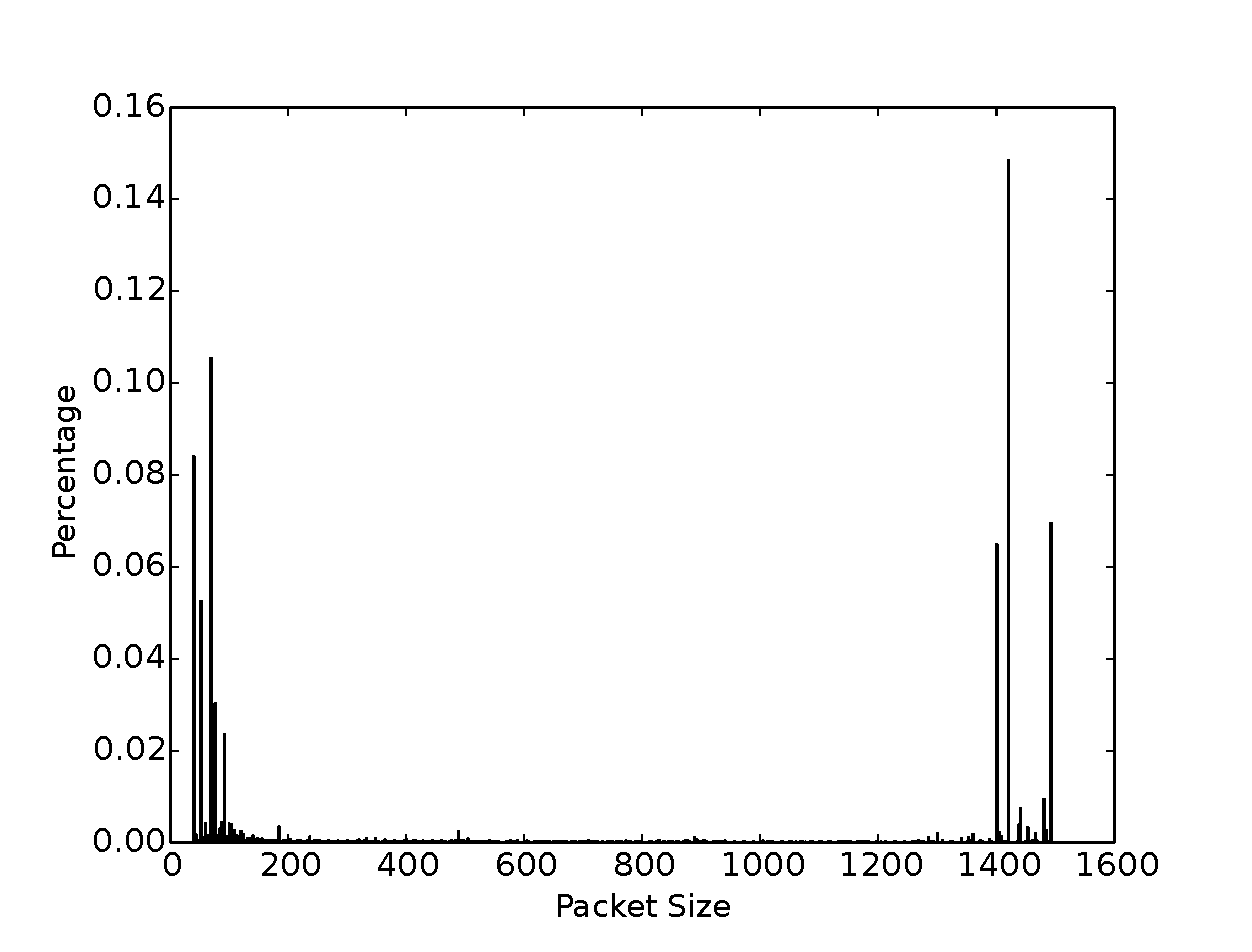
\includegraphics[width=\linewidth]{image/ssh_pkt_size_downstream.eps}
\caption{SSH, downstream}
\label{fig:ssh_pkt_size_downstream}
\end{subfigure}
\begin{subfigure}{.24\linewidth}
\centering
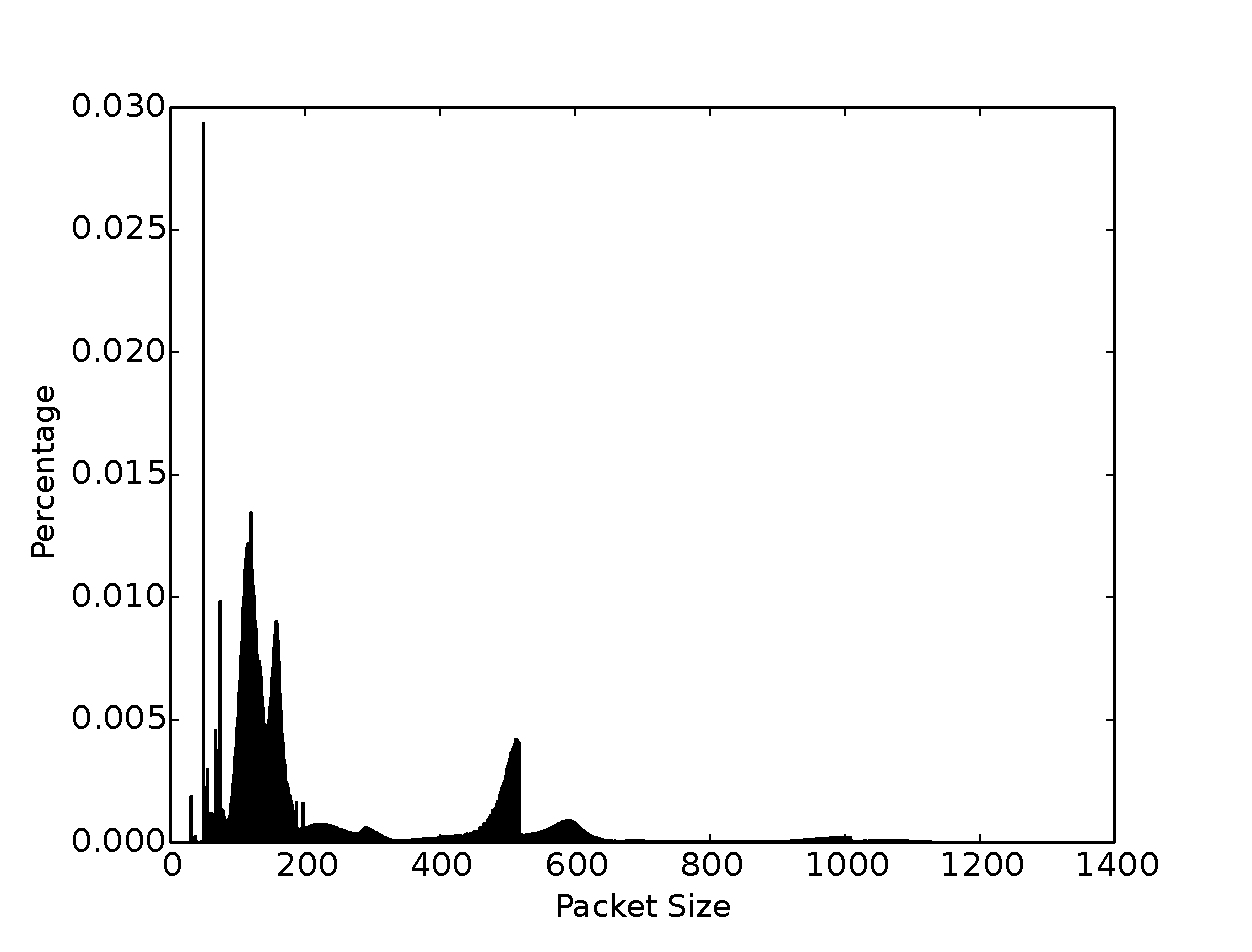
\includegraphics[width=\linewidth]{image/voip_pkt_size_upstream.eps}
\caption{VoIP, upstream}
\label{fig:voip_pkt_size_upstream}
\end{subfigure}
\begin{subfigure}{.24\linewidth}
\centering
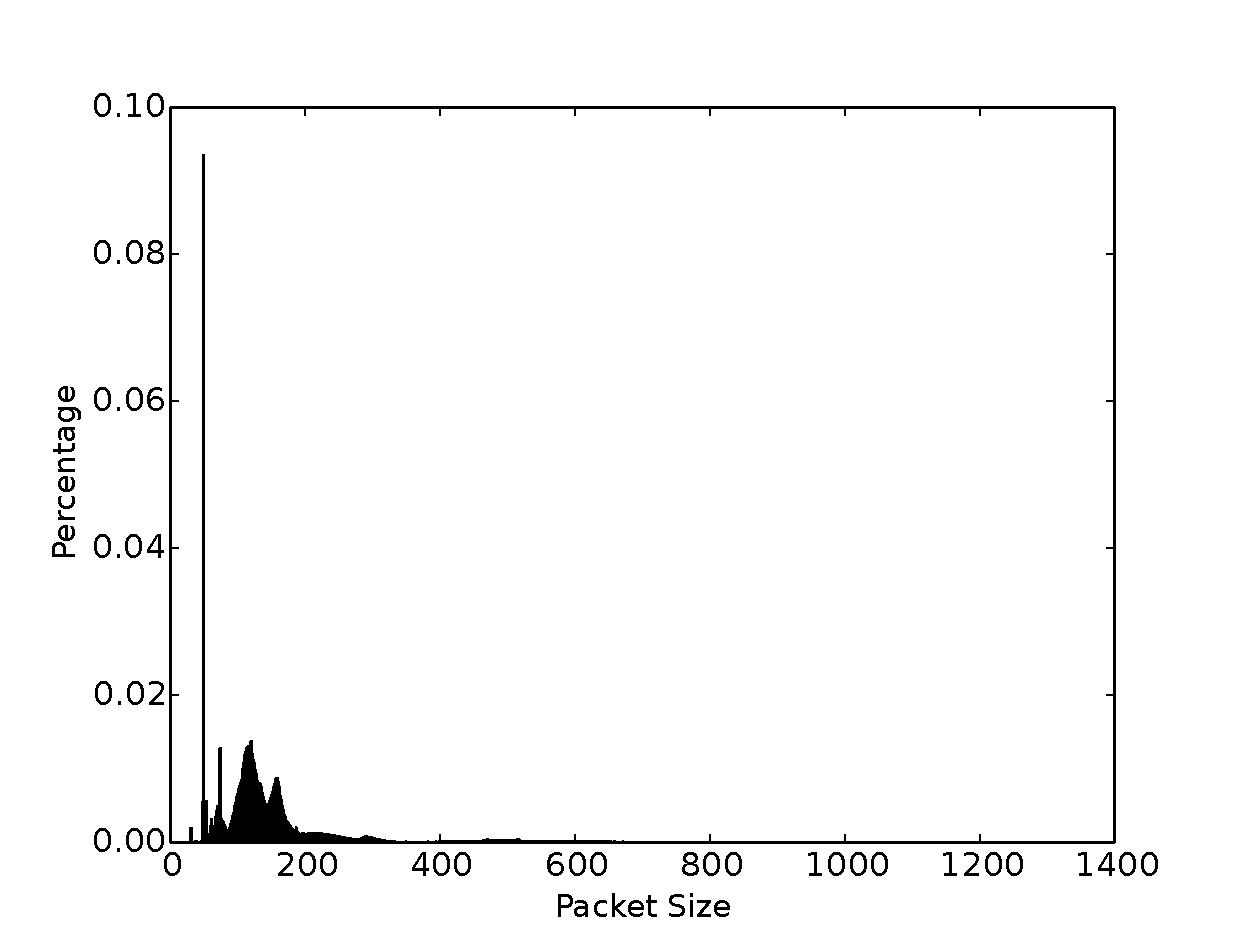
\includegraphics[width=\linewidth]{image/voip_pkt_size_downstream.eps}
\captionof{figure}{VoIP, downstream}
\label{fig:voip_pkt_size_downstream}
\end{subfigure}
%\begin{subfigure}{.24\linewidth}
%\centering
%\includegraphics[width=\linewidth]{image/%bittorrent_pkt_size_upstream.eps}
%\caption{BitTorrent, upstream}
%\label{fig:bittorrent_pkt_size_upstream}
%\end{subfigure}
%\begin{subfigure}{.24\linewidth}
%\centering
%\includegraphics[width=\linewidth]{image/%bittorrent_pkt_size_downstream.eps}
%\caption{BitTorrent, downstream}
%\label{fig:bittorrent_pkt_size_downstream}
%\end{subfigure}
\caption{Upstream and downstream packet size distribution of \bc and several popular protocols}\label{fig:traff-hist}
\end{figure*}
%\end{comment}
%\subsection{Ratio of Downstream to Upstream}\label{apend:ratio}

We start by characterizing \bc's traffic patterns. 

\subsection{Proportion and Distribution of Messages} \label{sec:prop_dist_msg}
\bc peers generate various kinds of messages as introduced in the previous section. 
We show that the distribution and sizes of such messages are quite unique to the \bc protocol, 
making \bc traffic easily distinguishable from other protocols. 

\begin{comment}
Table~\ref{table:msg_proportion} demonstrates the proportion of different messages in the \bc traffic we collected 
for 31 days. As can be seen, \code{tx} and \code{inv} are dominating with 43.6\% and 27.2\% of all packets, respectively. 
Therefore, the characteristics of these messages will shape the pattern of a \bc peer's traffic. 
\end{comment}


\paragraphb{Distribution of packet sizes.}
Figures~\ref{fig:inv_pktsizes} to~\ref{fig:tx_pktsizes} illustrate
the  packet size histogram of 
different types of \bc messages in our collected \bc traffic.
As can be seen, each type of message has a distinguishing traffic pattern. Note that through our experiments, we find out that \code{tx} and \code{inv} are dominating with 43.6\% and 27.2\% of all packets, respectively. 
Therefore, the characteristics of these messages will shape the pattern of a \bc peer's traffic. 


\paragraphb{Histogram of packet sizes in aggregate traffic.}
Figures~\ref{fig:aggregate_pkt_size_upstream_cmpct} and~\ref{fig:aggregate_pkt_size_downstream_cmpct} show the histogram of packet sizes in the upstream and downstream directions, respectively, in compact block relaying. 
As mentioned before, \code{tx} and \code{inv} dominate the messages sent by a typical \bc peer, therefore their sizes 
(shown in Figures~\ref{fig:inv_pktsizes} and \ref{fig:tx_pktsizes}) strongly shape the histogram of \bc traffic, making it uniquely distinguishable from other protocols. 

We also show the histogram of \bc traffic in the full block relaying mode in Figures~\ref{fig:aggregate_pkt_size_upstream_full} and~\ref{fig:aggregate_pkt_size_downstream_full}. These histograms have a larger spike close to the MTU, unlike the case of compact block relaying. These are because of the larger block sizes (around 1MB) in the full block relaying. 

\paragraphe{Comparing to other protocols:}
Figures~\ref{fig:http_pkt_size_upstream} to~\ref{fig:voip_pkt_size_downstream}  show the histogram of other popular protocols, collected as described in Section~\ref{sec:exp-dataset}. Note that we look at the traffic after going through an encryption tunnel, e.g., a VPN or SSH tunnel, so the histogram includes the (small) TCP ACK packets. 
As we can see, 
the packet size distribution of \bc is uniquely different from these other protocols, since a \bc connection is composed of unique messages with specific size distributions shown before. For instance, the large number of \code{inv} messages shapes the overall distribution of sizes in \bc traffic. 

 

\paragraphb{Ratio of downstream to upstream.}
We also measured the ratio of downstream to upstream traffic volumes, which is shown in Figure~\ref{fig:ratio_downstream_upstream_traffic_volume_bitcoin}.
Unlike other protocols like HTTP (shown in
Figures~\ref{fig:ratio_downstream_upstream_traffic_volume_http} to \ref{ratio_downstream_upstream_traffic_volume_bittorrent}),
\bc traffic has a \emph{symmetric} traffic volume in upstream and downstream. 
This is due to the fact that \bc peers broadcast most of the bulky protocol messages they receive such as block and transaction announcements. 


\subsection{Shape of Traffic}\label{sec:shape_of_traffic}

Above we showed that the counts and sizes of packets in \bc demonstrate a unique behavior. 
Here we show that, additionally, the shape of \bc traffic is distinguishable from other protocols.


\begin{figure*}
\centering
\begin{subfigure}{0.32\linewidth}
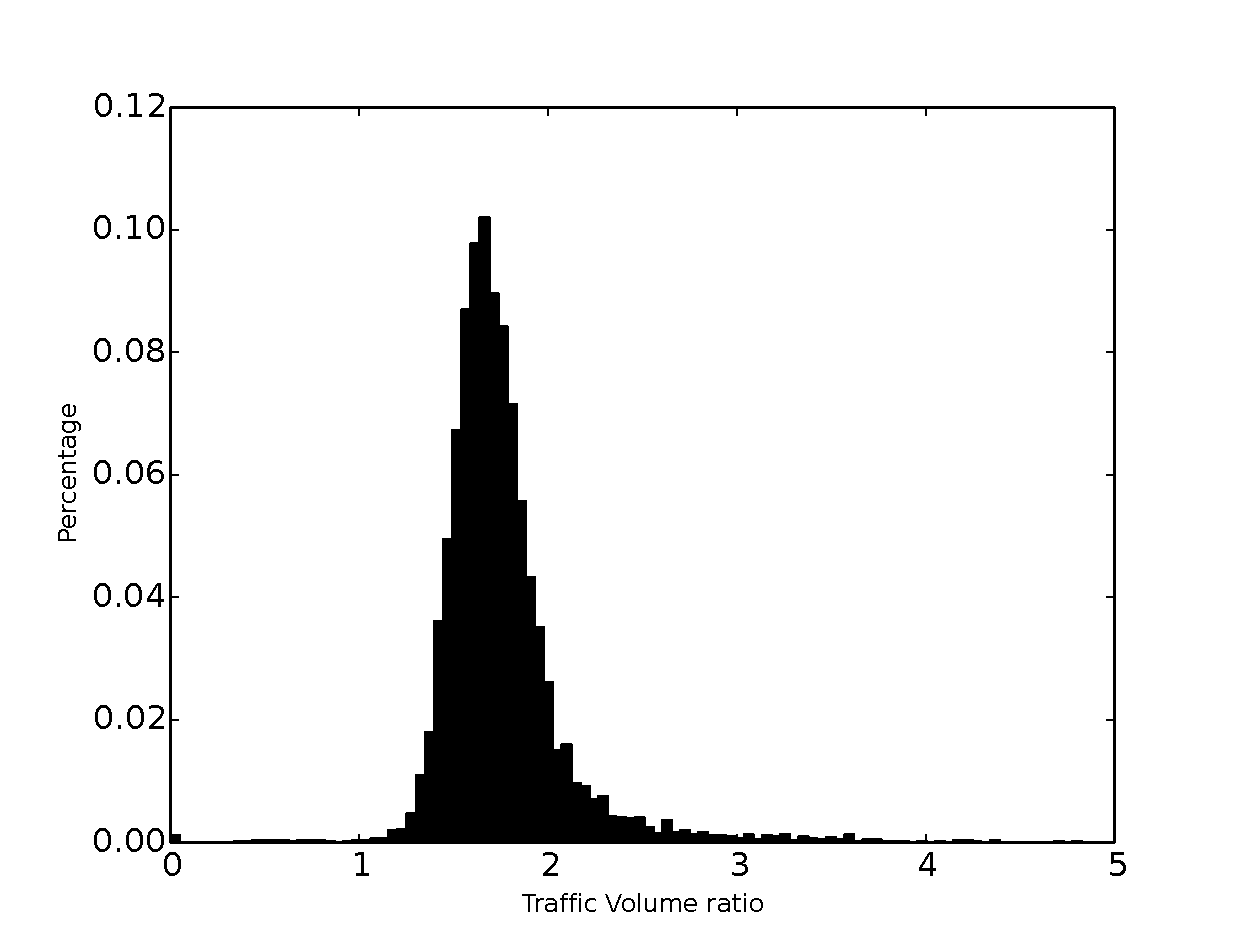
\includegraphics[width=\linewidth]{image/ratio_downstream_upstream_traffic_volume_bitcoin.eps}
\caption{Bitcoin, ratio per 5 minutes traffic}
\label{fig:ratio_downstream_upstream_traffic_volume_bitcoin}
\end{subfigure}
\begin{subfigure}{0.32\linewidth}
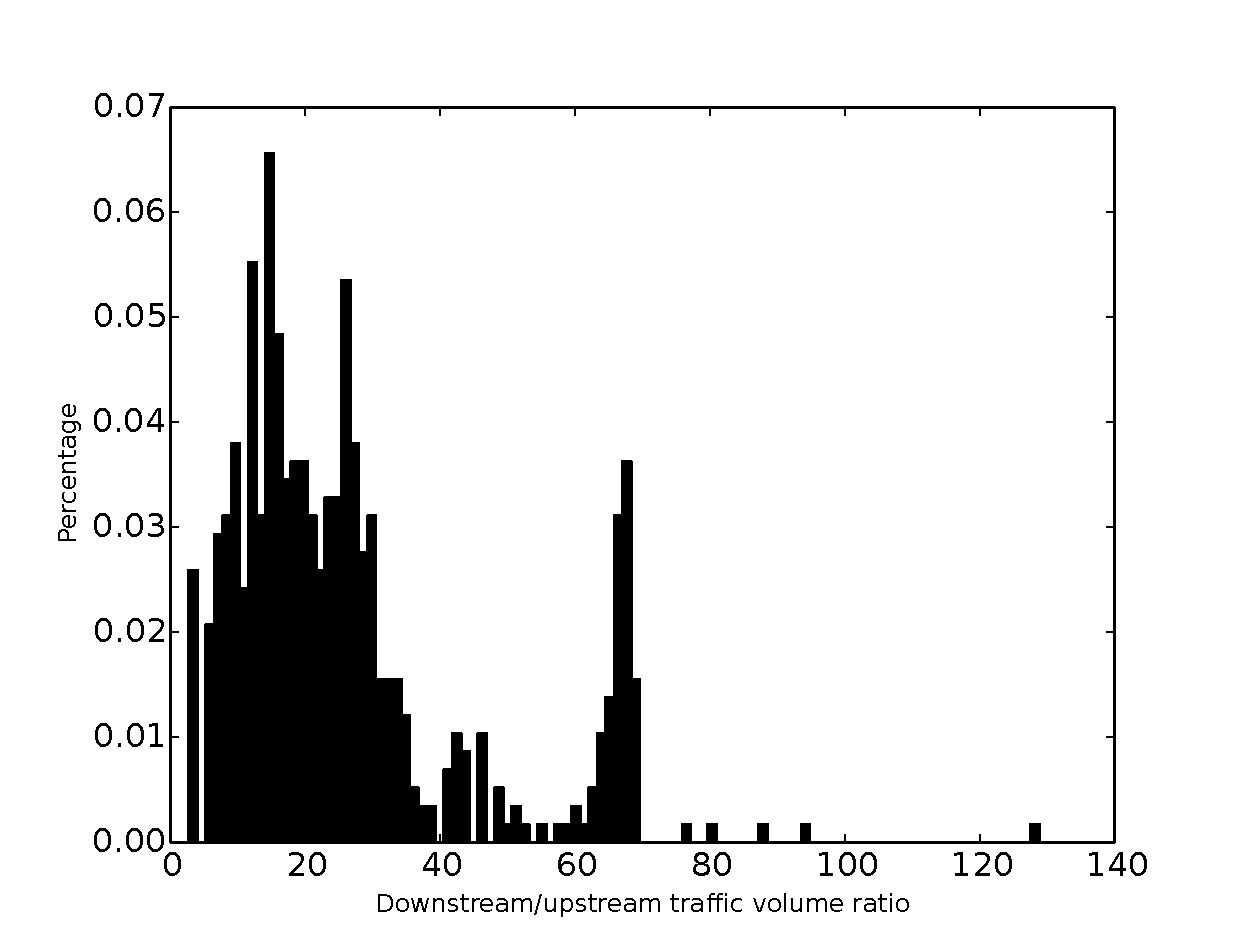
\includegraphics[width=\linewidth]{image/ratio_downstream_upstream_traffic_volume_http.eps}
\caption{HTTP, ratio per website}
\label{fig:ratio_downstream_upstream_traffic_volume_http}
\end{subfigure}
\begin{subfigure}{0.32\linewidth}
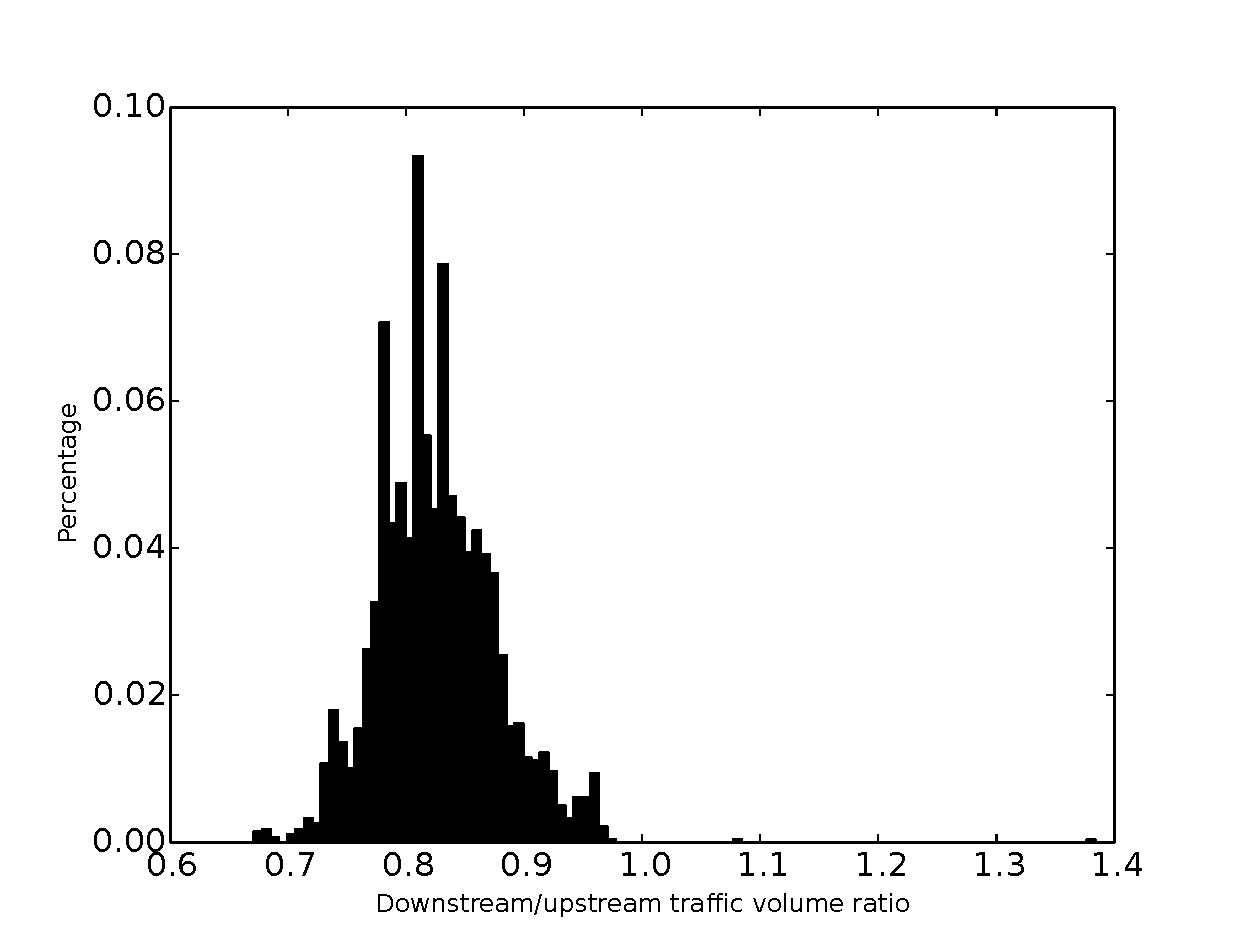
\includegraphics[width=\linewidth]{image/ratio_downstream_upstream_traffic_volume_ftp.eps}
\caption{FTP, ratio per 5 minutes traffic}
\label{ratio_downstream_upstream_traffic_volume_ftp}
\end{subfigure}
\begin{subfigure}{0.32\linewidth}
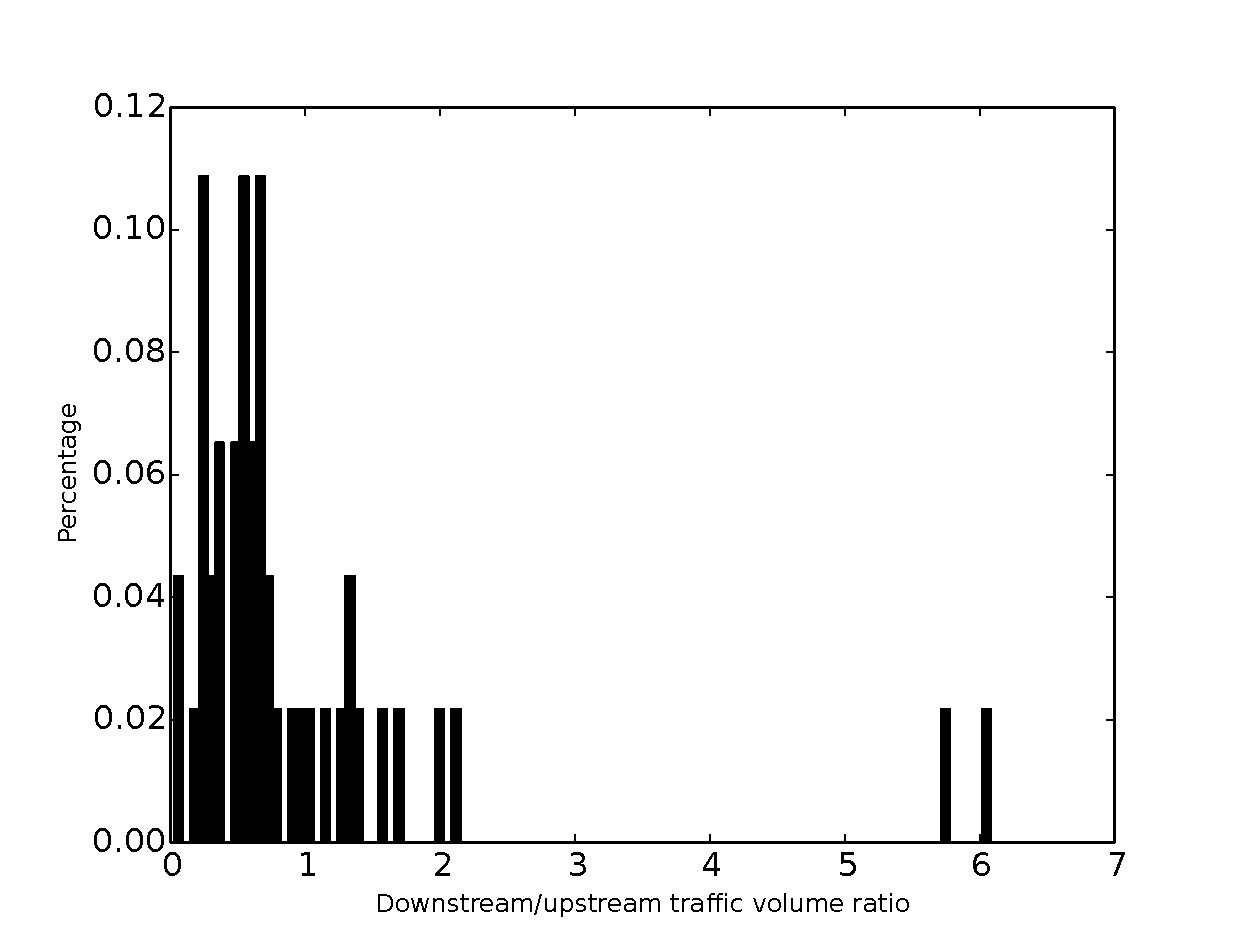
\includegraphics[width=\linewidth]{image/ratio_downstream_upstream_traffic_volume_ssh.eps}
\caption{SSH, ratio per 1 minute traffic}
\label{ratio_downstream_upstream_traffic_volume_ssh}
\end{subfigure}
\begin{subfigure}{0.32\linewidth}
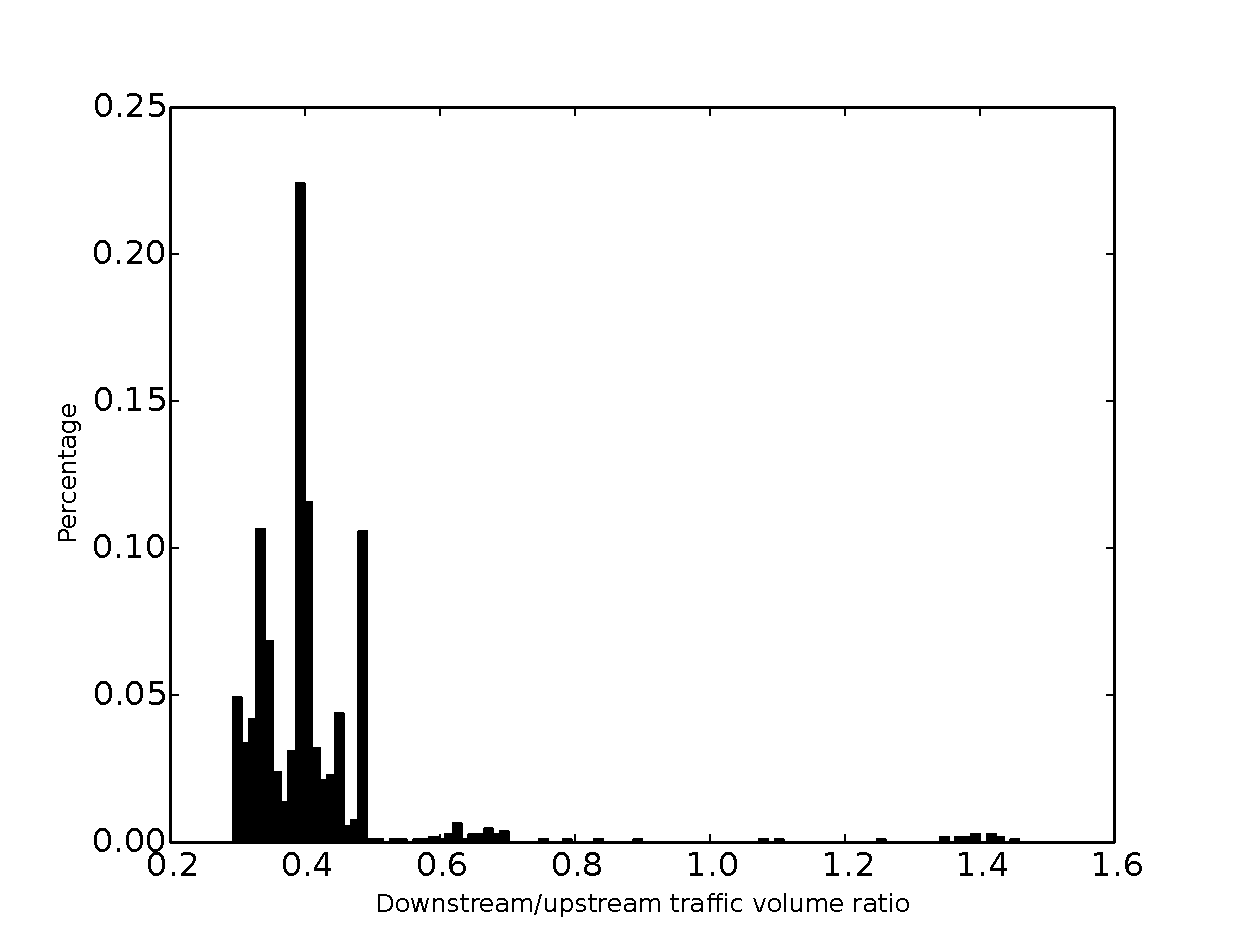
\includegraphics[width=\linewidth]{image/ratio_downstream_upstream_traffic_volume_voip.eps}
\caption{VoIP, ratio per 5 minutes traffic}
\label{ratio_downstream_upstream_traffic_volume_voip}
\end{subfigure}
\begin{subfigure}{0.32\linewidth}
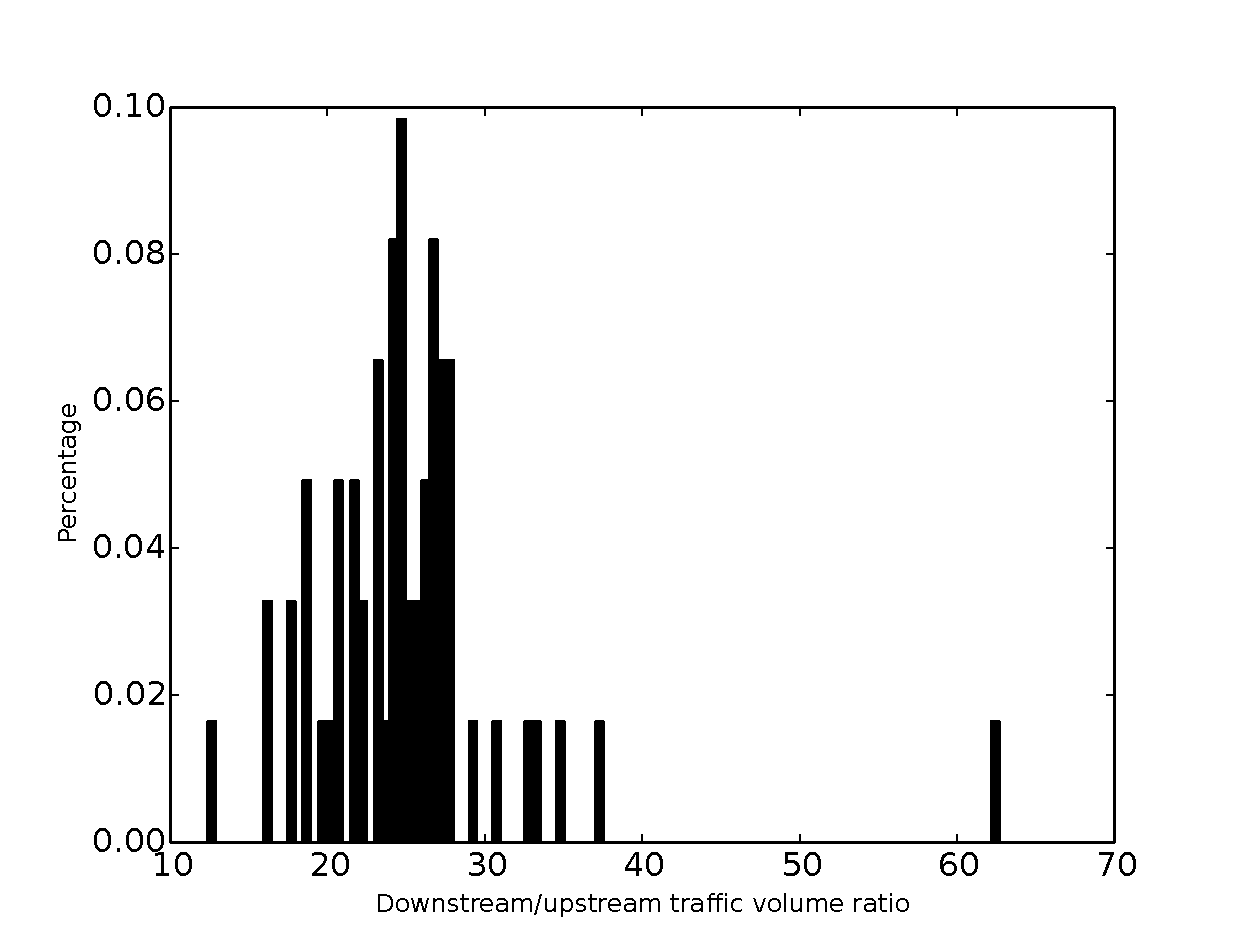
\includegraphics[width=\linewidth]{image/ratio_downstream_upstream_traffic_volume_bittorrent.eps}
\caption{BitTorrent, ratio per 5 minutes traffic}
\label{ratio_downstream_upstream_traffic_volume_bittorrent}
\end{subfigure}
\caption{Ratio of downstream to upstream traffic volume}
\end{figure*}

\paragraphb{Full block relaying mode:} 
Figure~\ref{fig:bitcoin_traffic_pattern} shows the traffic of a \bc client operating in the full block relaying mode.
As can be seen, the small protocol packets, mostly corresponding to \code{inv} and \code{tx} messages, appear 
uniformly over the time. 
On the other hand, the \bc full blocks appear as large spikes of roughly 1MB at specific points in time, i.e., once a new block is generated in the network. 

\paragraphb{Compact block relaying mode:}
In the compact block relaying mode, it is harder to notice the block spikes 
since only a sketch of the blocks is transmitted. In this mode, transmitting a compact block in the network results in smaller spikes of 100KB. Spikes of such small sizes may also occur when unverified transactions are transmitted, which will increase the detection's false positive. Also, a \bc client may operate in the high bandwidth mode, in which the receiver node  asks its peers to send new blocks without asking for permissions first. This will lead to more than one peer sending the same block at the same time. This and the large volume of missed transactions result in having spikes with more than 100 KB in the traffic. 
Figure~\ref{fig:cmpctblock_traffic_volume_detectable} illustrates  when and how
compact blocks appear on a peer's traffic. As can be seen, compact blocks appear at
smaller amplitudes than the actual block size, but the behavior is also nondeterministic,
since it depends on whether the client has previously received some of the transactions
in that block. This intuitively makes detection of compact blocks less reliable than full blocks, as shown later in our experiments. 

We also measure the size of compact blocks by measuring the 
\textit{length} field of \code{cmpctblock} messages, which is shown in Figure~\ref{fig:cmpctblock_traffic_volume}. 
As can be seen, most of the compact blocks are as small as 15 KB (in contrast to 1MB in full blocks). 

 \begin{figure*}[!t]
\begin{subfigure}{.48\linewidth}
\centering
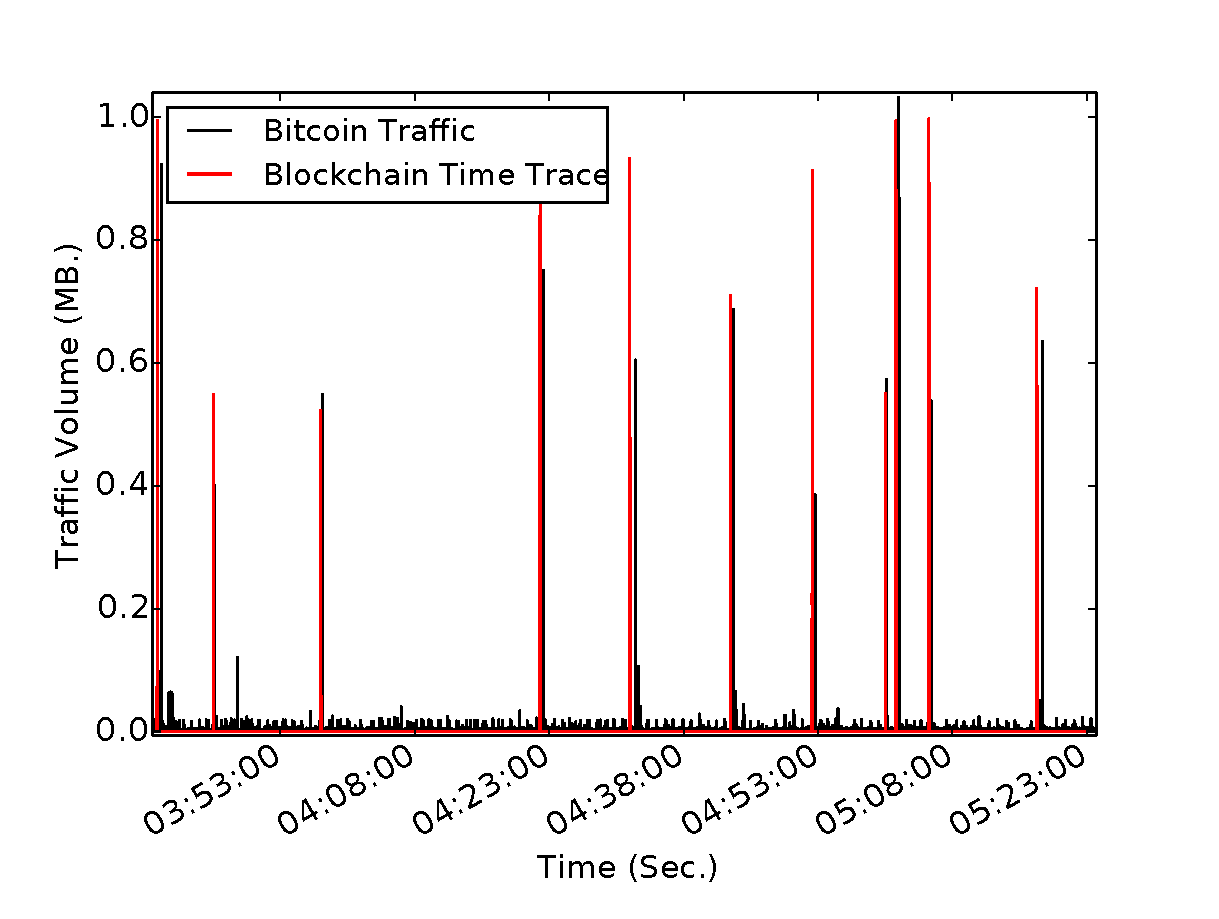
\includegraphics[width=0.9\linewidth]{image/bitcoin_traffic_pattern.pdf}
\caption{Full block}
\label{fig:bitcoin_traffic_pattern}
\end{subfigure}
\centering
\begin{subfigure}{.48\linewidth}
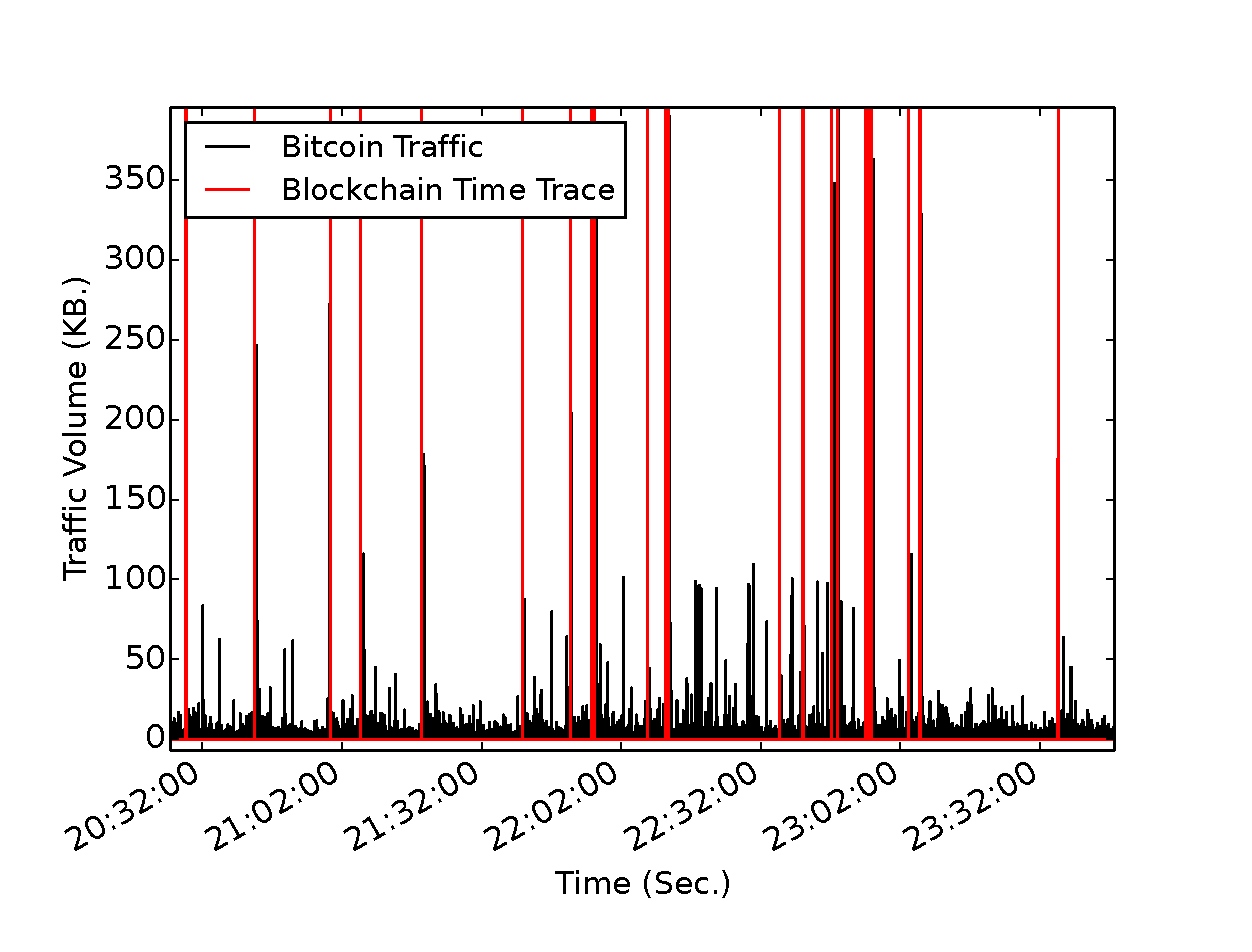
\includegraphics[width=0.9\linewidth]{image/cmpctblock_traffic_volume_good.eps}
\caption{Compact block}
\label{fig:cmpctblock_traffic_volume_detectable}
\end{subfigure}
\caption{Comparing time of each block receive with time of blocks in the block chain in a) Full block and b) Compact block modes}
\end{figure*}

%\Q{Not quite sure what this is , and why we need this. Maybe elaborate?}\A{So this figure is showing the volume of transactions which the receiving haven't had and will receive it by \code{blocktxn} message, since it will send to receiving node after sending the compact block it also may have impact on the traffic volume at the point that we are expecting a block. }
Finally, we measure the volume of transactions missing from an announced compact block (we do so based on the payload length of \code{blocktxn} messages).
As described earlier,  a \bc client operating in the compact block mode will download such missing transactions.
%We measure the missing transactions based on the the payload length of \code{blocktxn} messages in the same way we measure the compact block sizes. 
This is shown in Figure~\ref{fig:blocktxn_volume}. 
As we can see most of the transactions have volumes less than 100 KB. 

 \begin{figure}[!t]
\begin{subfigure}{.48\linewidth}
\centering
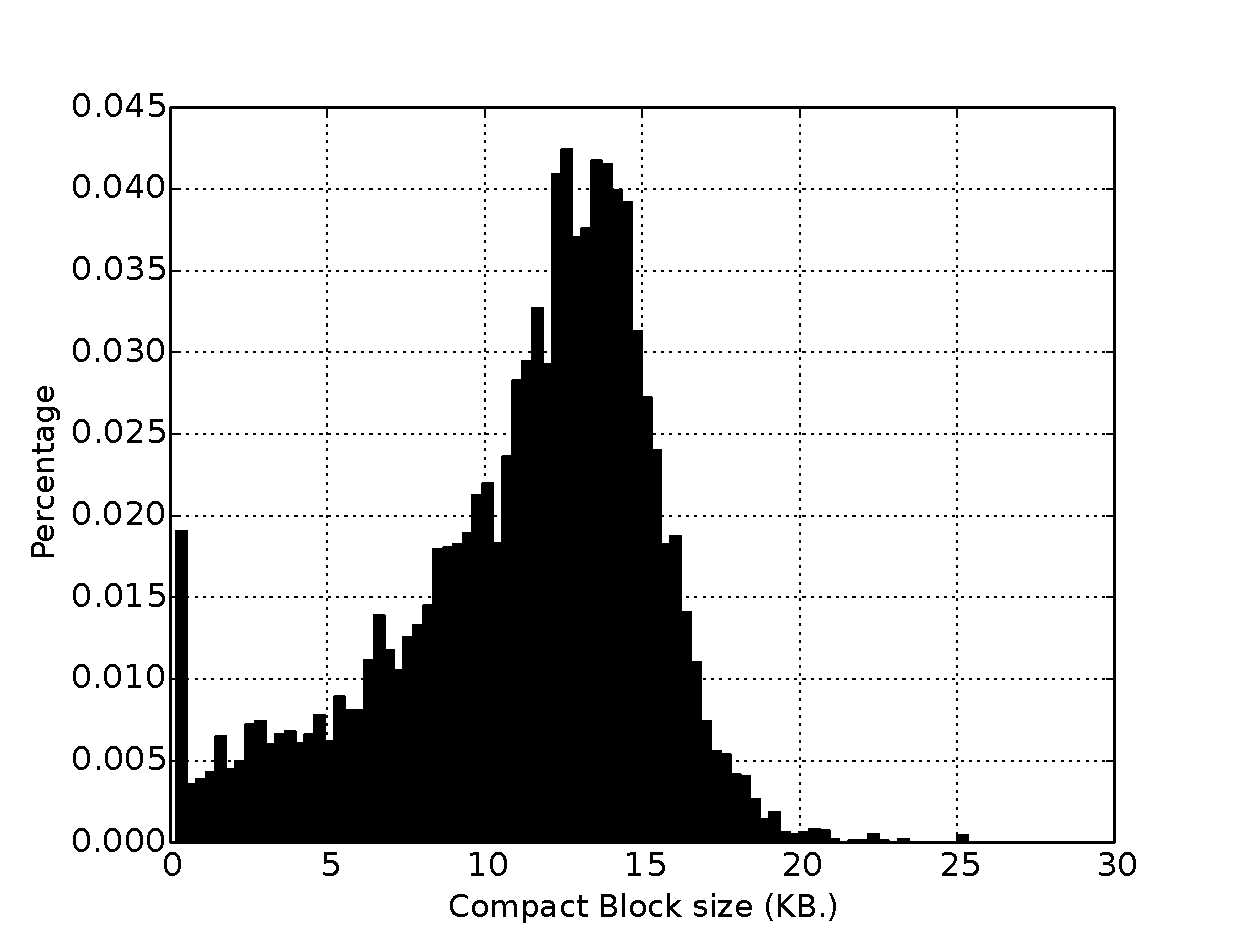
\includegraphics[width=0.9\linewidth]{image/cmpctblock_traffic_volume.eps}
\caption{Histogram of the size of compact blocks}
\label{fig:cmpctblock_traffic_volume}
\end{subfigure}
\centering
\begin{subfigure}{.48\linewidth}
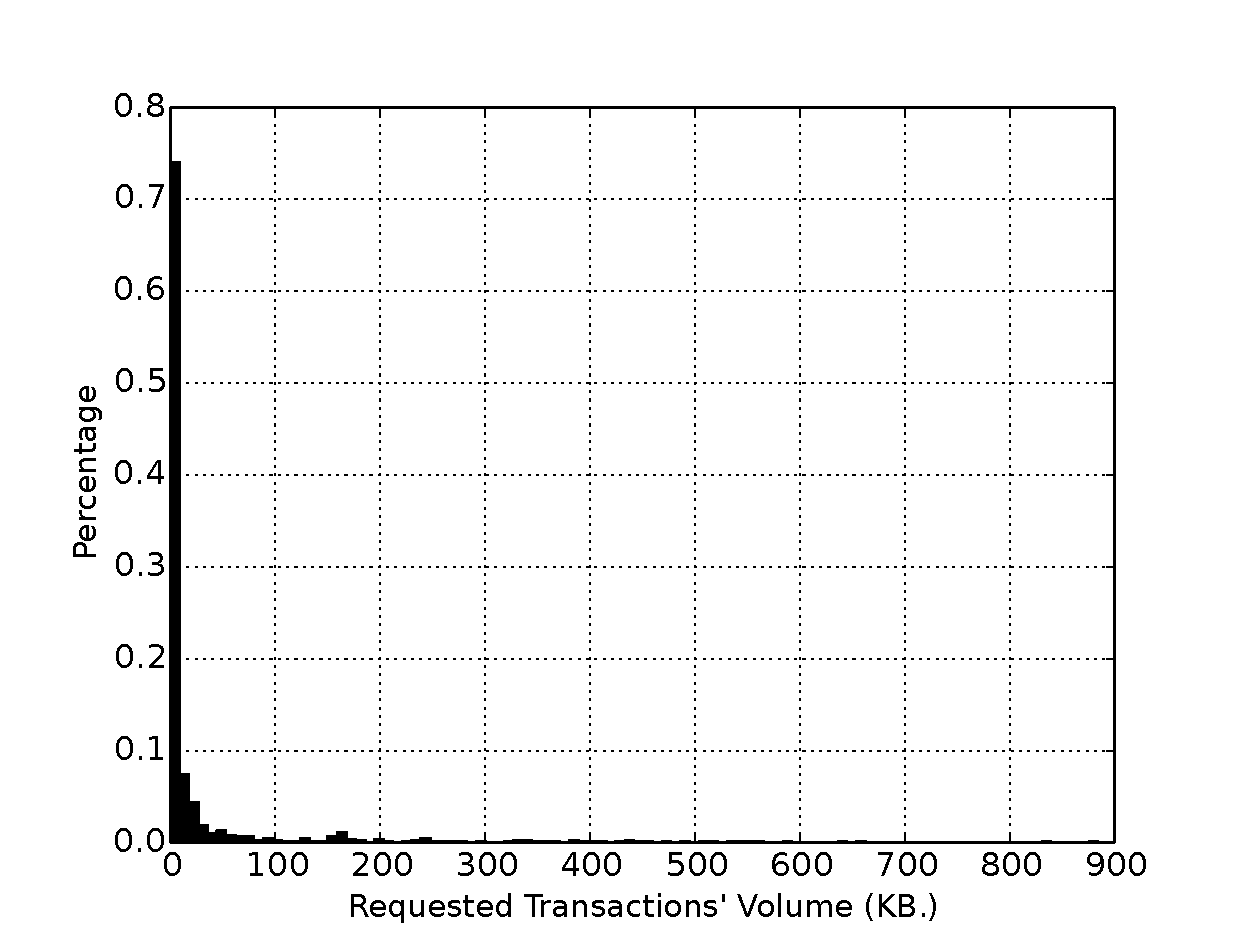
\includegraphics[width=0.9\linewidth]{image/blocktxn_volume.eps}
\caption{Histogram of the size of missing transactions}
\label{fig:blocktxn_volume}
\end{subfigure}
\caption{Histogram of compact block mode components}
\label{fig:hist_cmp_component}
\end{figure}

%The client's traffic shows a specific pattern, which makes us enable to come up with an algorithm to distinguish the Bitcoin traffic. We used our analysis in block propagation delay and Bitcoin traffic analysis to propose a correlation scheme. With the means of our correlation scheme we introduce a scheme to detect Bitcoin traffic.


%%%%%%%%%

\paragraphb{Block propagation latencies.} The propagation delay in the Bitcoin network is due to transmission delays and block verification by the receiving node at each hop. The transmission delay is the time to exchanging \code{inv} and \code{get data} messages, and sending the block via a \code{block} message. 
 We measure block propagation delay by subtracting the receiving time of the block message and the time stamp in the header of the block message. Figures~\ref{fig:cmpctblock_time_difference} and \ref{fig:prop_delay} show the histogram of propagation delay for  $6000$ blocks in compact block and full block relaying, respectively. 
As shown in the figures, we can model this empirical data using a Beta distribution~\cite{probabilitybook}. %We choose a maximum for propagation delay such that $99\%$ of beta distribution is below that maximum. According to our measurements this value equals to $65$ seconds.\fatemeh{rewrite this part}

\begin{figure}[!t]% to have a bigger picture just add * at the end of figure
\begin{subfigure}{.48\linewidth}
\centering
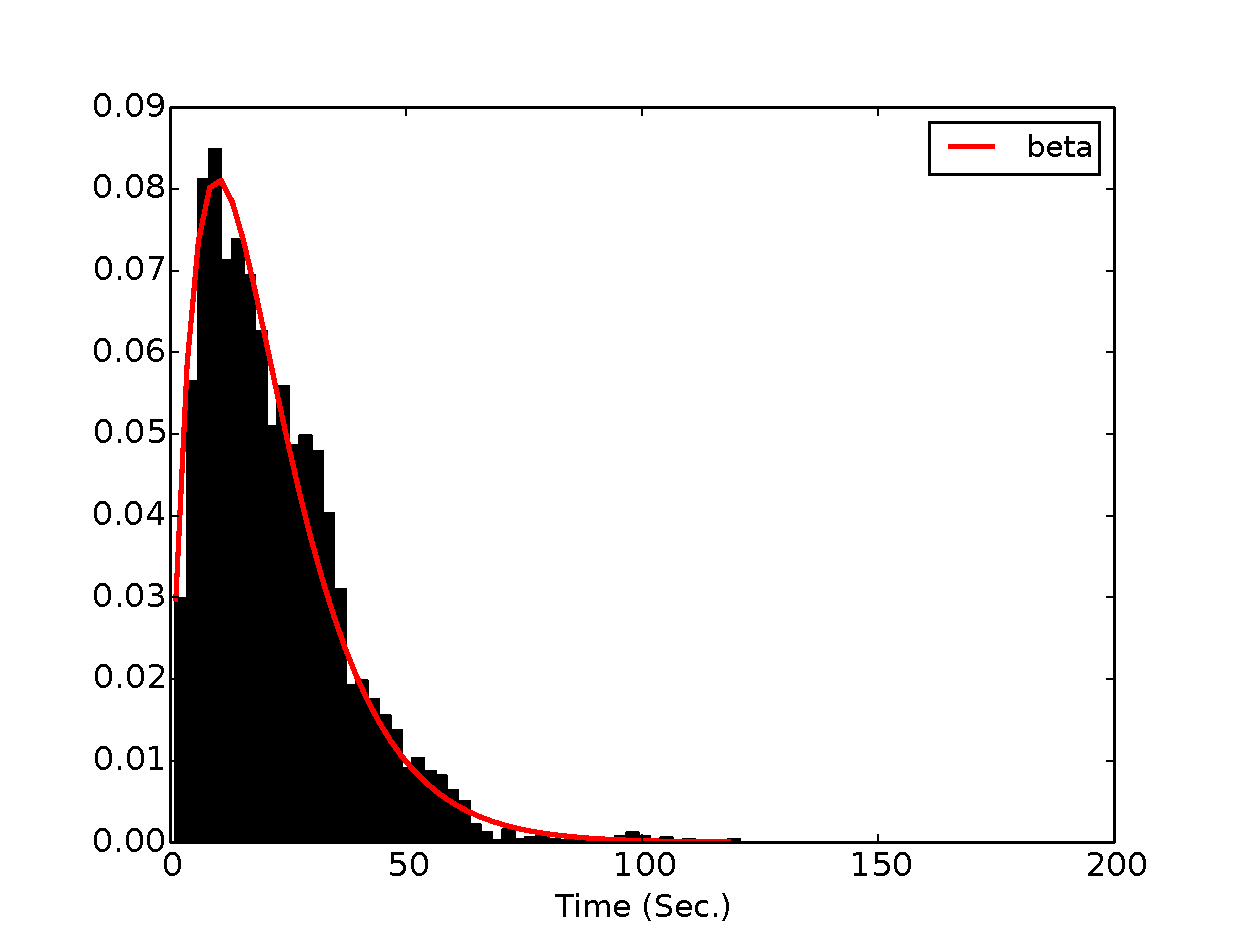
\includegraphics[width=0.9\linewidth]{image/cmpctblock_time_difference.eps}
\caption{Compact block}
\label{fig:cmpctblock_time_difference}
\end{subfigure}
\centering
\begin{subfigure}{.48\linewidth}
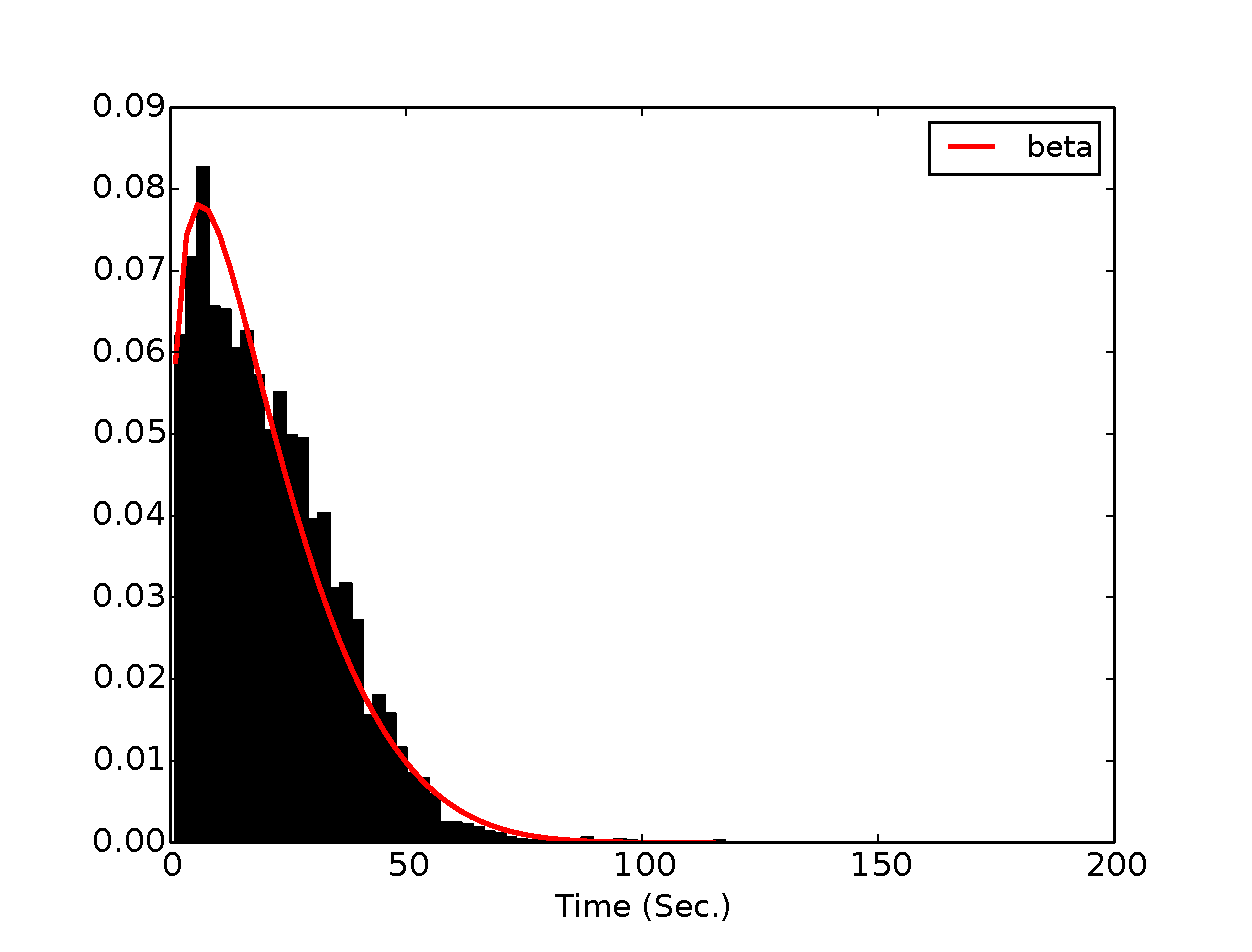
\includegraphics[width=0.9\linewidth]{image/prop_delay_beta.eps}
\caption{Full block}
\label{fig:prop_delay}
\end{subfigure}
\caption{Histogram of block propagation delays}
\label{fig:prop_delay_full_compact}
\end{figure} 



%\paragraphb{Traffic patterns.} 
%In traditional block relaying, full block relaying, the client which its ledger is updated tries to download each block whenever they are announced to the client. Since at the time of writing this paper the block size is 1 MB, downloading full blocks causes a sudden burst in the traffic of network.
%
%\par Figure \ref{fig:bitcoin_traffic_pattern} shows the traffic of a client which is connected to Bitcoin network which relays full blocks. As we can see whenever we have a Bitcoin block in block-chain time trace there is a significant burst in the client traffic. 



%In the compact block relaying, since only a sketch of block is transmitted and there is no 1 MB bursts in the traffic, finding spikes would be harder. 



%%%%%%%%%%%%%%%%%%%%%%%%%%%%%%%%%%%%%%%%%%%%%%%%%%%%%%%%%%%
%%%%%%%%%%%%%%%%%%%%%%%%%%%%%%%%%%%%%%%%%%%%%%%%%%%%%%%%%%%
%%%%%%%%%%%%%%%%%%%%%%%%%%%%%%%%%%%%%%%%%%%%%%%%%%%%%%%%%%%
\section{Designing \bc Classifiers}
We use the features described above to build robust classifiers for \bc traffic. 
We aim for our classifiers to work even in the presence of encryption and background traffic, e.g., 
when the machine running \bc is used for web browsing and runs other applications, or when the \bc traffic is tunneled over Tor. %user's traffic is mixed with the traffic of other users in a big VPN connection. 
%For a target connection, our classifiers extract specific features from it, using which decide if the target traffic contains \bc or not. Each of our classifiers extract certain features as introduced below. We evaluate the performance of our classifiers using false positive, true positive and accuracy.

\subsection{Size-based Classifier}
As noted in Section~\ref{sec:prop_dist_msg}, the histogram of \bc packet sizes has a unique pattern. Based on this, we designed  classifiers to distinguish \bc traffic from other protocols. 

\subsubsection{Size histogram classifier (\code{SizeHist})}\label{sec:all-packet-size-classifier}

This classifier correlates the packet size histogram of a target user's traffic with the packet size histogram of \bc traffic captured by the adversary. By histogram of packet sizes we mean number of each packet size from 1 to \textit{MTU} size. To do so, the classifier first divides the given traffic into upstream and downstream directions, then it calculates the histogram of packet sizes in each direction. The baseline (real-time \bc traffic) is also divided in upstream and downstream directions. 

In the next step, the classifier calculates the cosine similarity between the histogram of the target traffic and several \bc traces in both upstream and downstream direction. If both of the upstream and downstream averaged correlation values are above their thresholds, the target traffic is detected as \bc traffic.

%Finally, to detect if the target traffic is \bc, the classifier compares the average of correlation values with a threshold.  %The thresholds are derived as shown in the experiments section. 
%\amir{where is this threshold discussed?} 
%\begin{algorithm}
\caption{Size histogram classifier}
\label{algo:pktsize_scheme}
\begin{algorithmic}[1]
\Procedure{Size Histogram Classifier}{}
\State $B_{dwn}, B_{up} \gets $ Size histogram of a Bitcoin downstream and upstream traffic
\State $V_{dwn}, V{up} \gets $ Size histogram of input downstream and upstream traffic
\State $cor_{dwn} = \frac{B_{dwn} . V}{|B_{dwn}|^2 \times |V_{dwn}|^2}$
%\State $B_{up} \gets $ Packet size histogram of a Bitcoin upstream traffic
%\State $V_{up} \gets $ Packet size histogram of input upstream traffic
\State $cor_{up} = \frac{B_{up} . V}{|B_{up}|^2 \times |V_{up}|^2}$
\State \Return $cor_{dwn}, core_{up}$
\EndProcedure
\end{algorithmic}
\end{algorithm}

% the error is bc of caption in these algorithms


\subsubsection{Tor-specific classifier (\code{SizeTor}):}

Tor~\cite{tor} reformats traffic into constant-sized segments called  \emph{cells}. However, as the size of a cell is smaller than the MTU of IP packets, depending on the volume of traffic, multiple cells can merge into one single packet. This makes the number of single-cell packets and multiple-cell packets different for different protocols tunneled over Tor. Our \code{SizeTor} classifier aims at detecting \bc traffic tunneled over Tor based on the distribution of single-cell packets. 
As shown in Appendix~\ref{sec:charachterzing_bc}, \bc traffic consists of a large number of small-size packets (due to frequent \code{inv} messages). Tor will add padding to these small packets to form cells. Therefore, the ratio of single-size packets in \bc over-Tor is larger than regular traffic over Tor, e.g., HTTP-over-Tor. Based on this, our classifier compares the ratio of single-cell packets to all packets; if the ratio is larger than a threshold, the connection will be flagged as a \bc connection. Note that our \code{SizeTor} classifier can be adjusted for other protocols that similarly change the size of packets.
\begin{comment}
\paragraph*{Tailoring for Tor Pluggable Transports}
 Through our experiments on \bc traffic over Tor pluggable Transports, we noticed that fraction of packets which have a specific size other than cell-size (for example, size $721$ in FTE ) are much larger than this value in normal traffic. Furthermore, this value is much larger than the fraction of packets which are in cell size. Therefore, when implementing sizeTor on pluggable transports, we compute the fraction of packets in these specific sizes to differentiate between \bc traffic and others.
\end{comment}
%\red{should combine with sizetor and rewrite}
%\paragraph*{SizeTor Extension}

\begin{comment}
\subsubsection{Downstream to upstream traffic volume ratio (\code{D2U})}
As we discussed in Appendix~\ref{sec:charachterzing_bc}, the ratio of downstream to upstream traffic volume is unique in \bc. This classifier looks at $t$ window of \bc traffic. The $t$ parameter should be at least $10$ minutes to include at least one block in it.
Then the downstream to upstream ratio is calculated for the target traffic. If the calculated ratio is smaller than a threshold, which is determined empirically, the traffic will be detected as \bc traffic. The threshold is defined in a way to distinguish \bc traffic from other traffic while minimizing false positive. This detection scheme will be effective even in the situation that the underlying system changes the packet sizes and packet timings, since the transmitted traffic volume in both directions would stay the same.
\end{comment}

\subsection{Shape-based Classifier}\label{window-sec}

%We demonstrated in Appendix~\ref{sec:shape_of_traffic} that the shape of \bc traffic is distinct from other protocols. 
%We therefore design classifiers that try to identify (encrypted) \bc traffic based on its shape. 
The main intuition of our shape-based classifier is looking for changes in the traffic volume of a target user around the times of block announcements. Therefore, we assume that the classifier obtains the times and sizes of \bc blocks, e.g., from the public \url{blockchain.info} repository, or even by running a local \bc client.

%Algorithm~\ref{algo:window_based_scheme} illustrates our shape-based correlation algorithm.
For each confirmed \bc block, the algorithm analyzes the volume of the target traffic two time windows with size $\omega_i$ around the block time, 
one before $(t_{block_i}-\omega_i, t_{block_i})$ and one after the block time $(t_{block_i}, t_{block_i} +\omega_i)$. The size of the window depends on the size of the block, the target client's bandwidth, etc., as evaluated later. 
%\begin{algorithm}[h]
\caption{Shape based classifier}
\label{algo:window_based_scheme}
\begin{algorithmic}[1]
\Procedure{ Shape based Classifier}{}
\State $B \gets $ Block-chain time trace extracted from blockchain.info 
\State $V \gets $ Captured traffic volume in 1 second epochs
\State $N \gets$ Total number of Blocks
\For{each block $b_i \in B$ }
\State $t_{b_i} \gets $ Time of generation of block $b_i$
%\State $\Delta \gets$ Block propagation delay 
\State $||b_i|| \gets $ Block's size
%\State $T = \frac{||b_i||}{bandwidth}$ 
%\State $window = T + \Delta$ 
\State $\omega_i \gets$ Window's size
\State $\Delta V_i = V(t_{b_i}, t_{b_i} +\omega_i) - V(t_{b_i}-\omega_i, t_{b_i})$ 

\If {$ ||b_i|| - J \leq \Delta V_i \leq ||b_i|| + J$ }
\State $detected\ block += 1$

\EndIf
\EndFor
\State \Return $\frac{detected\ block}{N}$
\EndProcedure
\end{algorithmic}

\end{algorithm}
For an actual \bc traffic with no noise, the difference should be close to the size of the block. 
%Therefore, the algorithm evaluates the difference of traffic volumes in the two consecutive windows and 
%compares it to a threshold determined by the natural network jitter of the target (as discussed later).
If the difference is within the bound ($J$), the algorithm considers that block to be \emph{detected} in the traffic of the suspected user. The algorithm performs the same for a number of blocks and evaluates the ratio of such ``detected'' blocks. 
If the ratio is above a threshold $\eta$, the target user is declared to be a \bc client. 
% the error is bc of caption in these algorithms


\paragraphb{Choosing the threshold $\eta$.} The threshold should be chosen based on the target user's specific network conditions such as background traffic, network noise, and bandwidth. %Therefore, the algorithm tailors the $\eta$ parameter for each specific user. 


To do so, the classifier generates $N$ (e.g., $N=100$) synthetic block series, which we call \emph{ground false}s. The classifier then correlates the target traffic with each of the $N$ ground false instances using the correlation function. Finally, the threshold $\eta$ is chosen to be larger than the largest correlation value.
%Each ground false is generated based on the known pattern of \bc blocks, e.g., by simulating blocks around 1MB roughly every 10 minutes for the full block relaying mode. More specifically, we generate the timing between blocks based on an Exponential distribution with mean 10 minutes.


\begin{comment}
\begin{align}\label{gt_gf}
\eta > \max(CF) 
\end{align}
%+ \alpha \ std(CF)
where $CF$ is the set of correlation values against the $N$ ground false instances. In another words, we choose $\eta$ to be larger than the largest correlation value.
\end{comment}

\paragraphb{Choosing other parameters.} The window shape classifier also needs to choose the values of the parameters $\omega$ and $J$. Parameter $\omega$ needs to be big enough to contain the most of the traffic of a block during block propagation. Moreover, Parameter $J$ is chosen to take into account that some  of the block propagation traffic might not be downloaded in that time window. This parameters needs to be selected based on user's bandwidth and the volume of background traffic, and therefore it needs to be chosen for each client specifically. 

% based
%on the features of the target user's traffic, e.g., her bandwidth and the volume of background traffic, and therefore it needs to be chosen for each client specifically. 
% The parameter $J$ represents natural network jitter for the target client and it should be chosen for each  client specifically.


\iffalse The window size parameter \textbf{\textit{$\omega$}} represents the delay for a client to fully receive a specific block. Therefore, it should be based on two features: propagation delay and download time. The propagation delay is usually smaller than the download time so we ignore it in choosing \textit{$\omega$}. 
We estimate a target client's block downloading time as $\frac{block\ size}{client's\ bandwidth}$.The parameter $J$ represents natural network jitter for the target client. To derive $J$ for each user, we derive the difference of traffic volume in the user's consecutive time windows, excluding the windows that arrive close to the times of blocks (note that we do not know if this is a \bc client or not). In other words, we measure $\Delta V$'s for windows that do not collide with block times.  
 $J$ is the standard deviation of such difference values.\fi

\subsection{Neural Network-based Classifier (NN-based)}\label{class:nn}
We use a neural network-based classifier to detect \bc in presence of a more complex background noise, e.g., browsing more than one website simultaneously. In following, we explain the feature selection phase, and then describe the design of our neural network.
\subsubsection{Feature selection}
%Again, we leverage the unique shape of \bc traffic as discussed before to classify \bc traffic using our NN-based classifier. 
To create each sample data, we divide time into intervals
and use the volume of traffic in each interval as our features, which is 
presented in equation $\mbox{vlm}=v_1, v_2, ..., v_{n}$. 

Note that $v_I$ is the volume of traffic in interval I. We choose $10$ minutes as the \textit{sample size}, which is the smallest length to have
at least one peak of traffic. Furthermore, to choose the interval
length, we try different values of $1$, $5$, $10$ and $20$ seconds. From our experiments, we find out 
that the interval length of $10$ seconds results in the best performance. Therefore, we choose $10$ 
seconds as the interval length ($l$). 
Since the length of each sample is $10$ minutes 
($600$ seconds), using equation $n=\mbox{sample size}/l$, we get an array of 
length $60$ as our feature.
\iffalse
\begin{equation}\label{eq:v}
 n=\mbox{sample size}/l
\end{equation}
\begin{equation}\label{eq:a}
\mbox{vlm}=v_1, v_2, ..., v_{n}
\end{equation}\fi
\subsubsection{Designing the model}
For our neural network model, we use a combination of convolutional and fully-connected network that 
consists of an input layer, an output layer, and three hiden layers: one convolutional layer, and two dense layers. The input layer has $n=60$ number of neurons, which is the size of each sample data, the hidden layers have $n_1=64$, $n_2=32$ and $n_3 = 16$ number of neurons, respectively, and the output layer has $1$ neuron which represents if the sample data contains \bc 
traffic or not. We use Relu as the activation function of the hidden layers and 
sigmoid~\cite{deep_learning_book} for the output layer. Also, we use binary cross-entropy as our loss function, and Adam optimization~\cite{adam}.% to minimize the loss. %The learning rate of the optimization 
%function is a hyperparameter of our model ( $lr$).

\subsection{Combined Classifier}
In this classifier, we combine all the attributes used in the above classifiers. More specifically, we are using the size histogram of the packets, downstream to upstream traffic volume ratio, and volume over time. Our final feature set has a length of $1576$ (1 for downstream to upstream, 60 for volume over time, and 1515 for size histogram). Note that the feature that we use in sizeTor classifier is a subset of size histogram, and volume over time is capturing the shape of traffic that we utilized in the shape-based classifier. The model that we use has three convolutional layers and one dense layer with sizes: $1024$, $128$, $64$, and $32$ for the dense layer. We use the same activation functions and loss function as the NN-based classifier.























\begin{comment}
\paragraphb{Extension to Compact Blocks}
%\subsubsection*{Compact Block Modification} \hfill \break
The classifier described above works best for the traditional full block relaying mode in which 
\bc peers receive the full blocks at the expected times. 
However, the correlation is weaker in the compact block relaying mode, 
since  only a sketch of each block will be downloaded by each peer, and the sketch will be different for different peers. 
We therefore need to adjust the parameters  of our classifier
(\textit{window size}, $J$) for compact block users. 


According to figure ~\ref{fig:cmpctblock_traffic_volume}, the volume of each compact block has an average of around 13 KB. This value will make the ratio $\frac{block\ size}{BW}$ negligible in comparison to $delta$. So, we consider $\omega$ approximately equal to $delta$. 
Since our experiments is for the high bandwidth mode, the receiving node might receive one block from multiple outgoing nodes. This will make the spike much larger than the average block size shown in Figure~\ref{fig:cmpctblock_traffic_volume}. Also, we consider the average volume of requested transactions. We calculate $\tau$ as follow:
\begin{align*}
\tau_i = 4 \times avg(compact\ block\ size) + avg(requested\ \code{txn}\ volume)
\end{align*}

We use a factor of 4 because in our setting we see that the client receives the transactions from 4 neighbors. 
\end{comment}



\section{Experimental Setup}\label{sec:exp-dataset}

We use Bitcoin Core software\footnote{https://bitcoin.org/en/bitcoin-core/} to run full node \bc clients on 5 virtual machines on a campus network. Each virtual machine is connected to the Internet with high bandwidth. Before starting the experiments, we leave our \bc clients for a few days to make sure they have downloaded an up-to-date blockchain ledger. The \bc client is passively receiving blocks and participating in the Bitcoin network, but it is not doing any transactions.
We capture \bc traffic under three different scenarios on a Linux $16.0.4$ virtual machine: 
%Following explains the traffic that we capture:
%\begin{compactitem}
\subsection{Datasets}
\paragraphb{Collecting \bc traffic:} We use \bc version 0.12.0 to capture \bc traffic in the full block relaying mode and Bitcoin version 0.14.0 to capture traffic in the compact block relaying mode. We capture \bc traffic for each version for a period of a month.
%Specifically, we captured the Bitcoin traffic in the full block relaying mode from August 28th to October 9th, 2016,  and \bc traffic in the compact block mode from March 14th to April 18th, 2017.

\paragraphb{\bc tunneled through Tor} We captured \bc traffic behind Tor~\cite{tor} for both compact and full block modes.
We also captured \bc traffic in the compact block mode behind %OpenVPN\footnote{https://openvpn.net/}, 
Tor and popular Tor pluggable transports of obfs4~\cite{obfs4}, FTE~\cite{fte}, and Meek-amazon~\cite{meek}.
%Furthermore, we capture \bc traffic tunneled through . 

\paragraphb{\bc with background traffic:} We captured \bc traffic in presence of HTTP background traffic by browsing the top 500 Alexa websites using the Selenium\footnote{\url{http://www.seleniumhq.org}} tool while running \bc software. We also collected \bc 
traffic with HTTP background for the same set of websites behind Tor and its three pluggable transports using Selenium.

\iffalse  \textbf{\bc traffic } in full and compact mode(30 days each). Also, \bc compact mode traffic over VPN, Tor and three pluggable transports(up to 20 days)\fi

\paragraphb{CAIDA background traffic:}
We use CAIDA's 2018 anonymized traces\footnote{\url{https://www.caida.org/data/monitors/passive-equinix-nyc.xml}} as a dataset for additional background traffic. 
%We extracted the flows in this database based on the protocol type, IP addresses and port numbers of the end-hosts. 
%For each IP address, we consider all traffic to and from that IP as the typical traffic of that user. Table~\ref{tab:traffic_class} shows the class breakdown of CAIDA dataset used in our experiments.

\paragraphb{HTTP traffic:}% (normal traffic, behind VPN and Tor)
We collect top $500$ Alexa websites using Selenium tool. Also, we capture these websites over Tor, and three pluggable transports. Moreover, we use 
the dataset by~\cite{deepcore} which has collected the top $50,000$ Alexa websites over Tor. 


%\end{compactitem}

\iffalse
\begin{figure}[!t]

\begin{subfigure}{.48\linewidth}
\centering
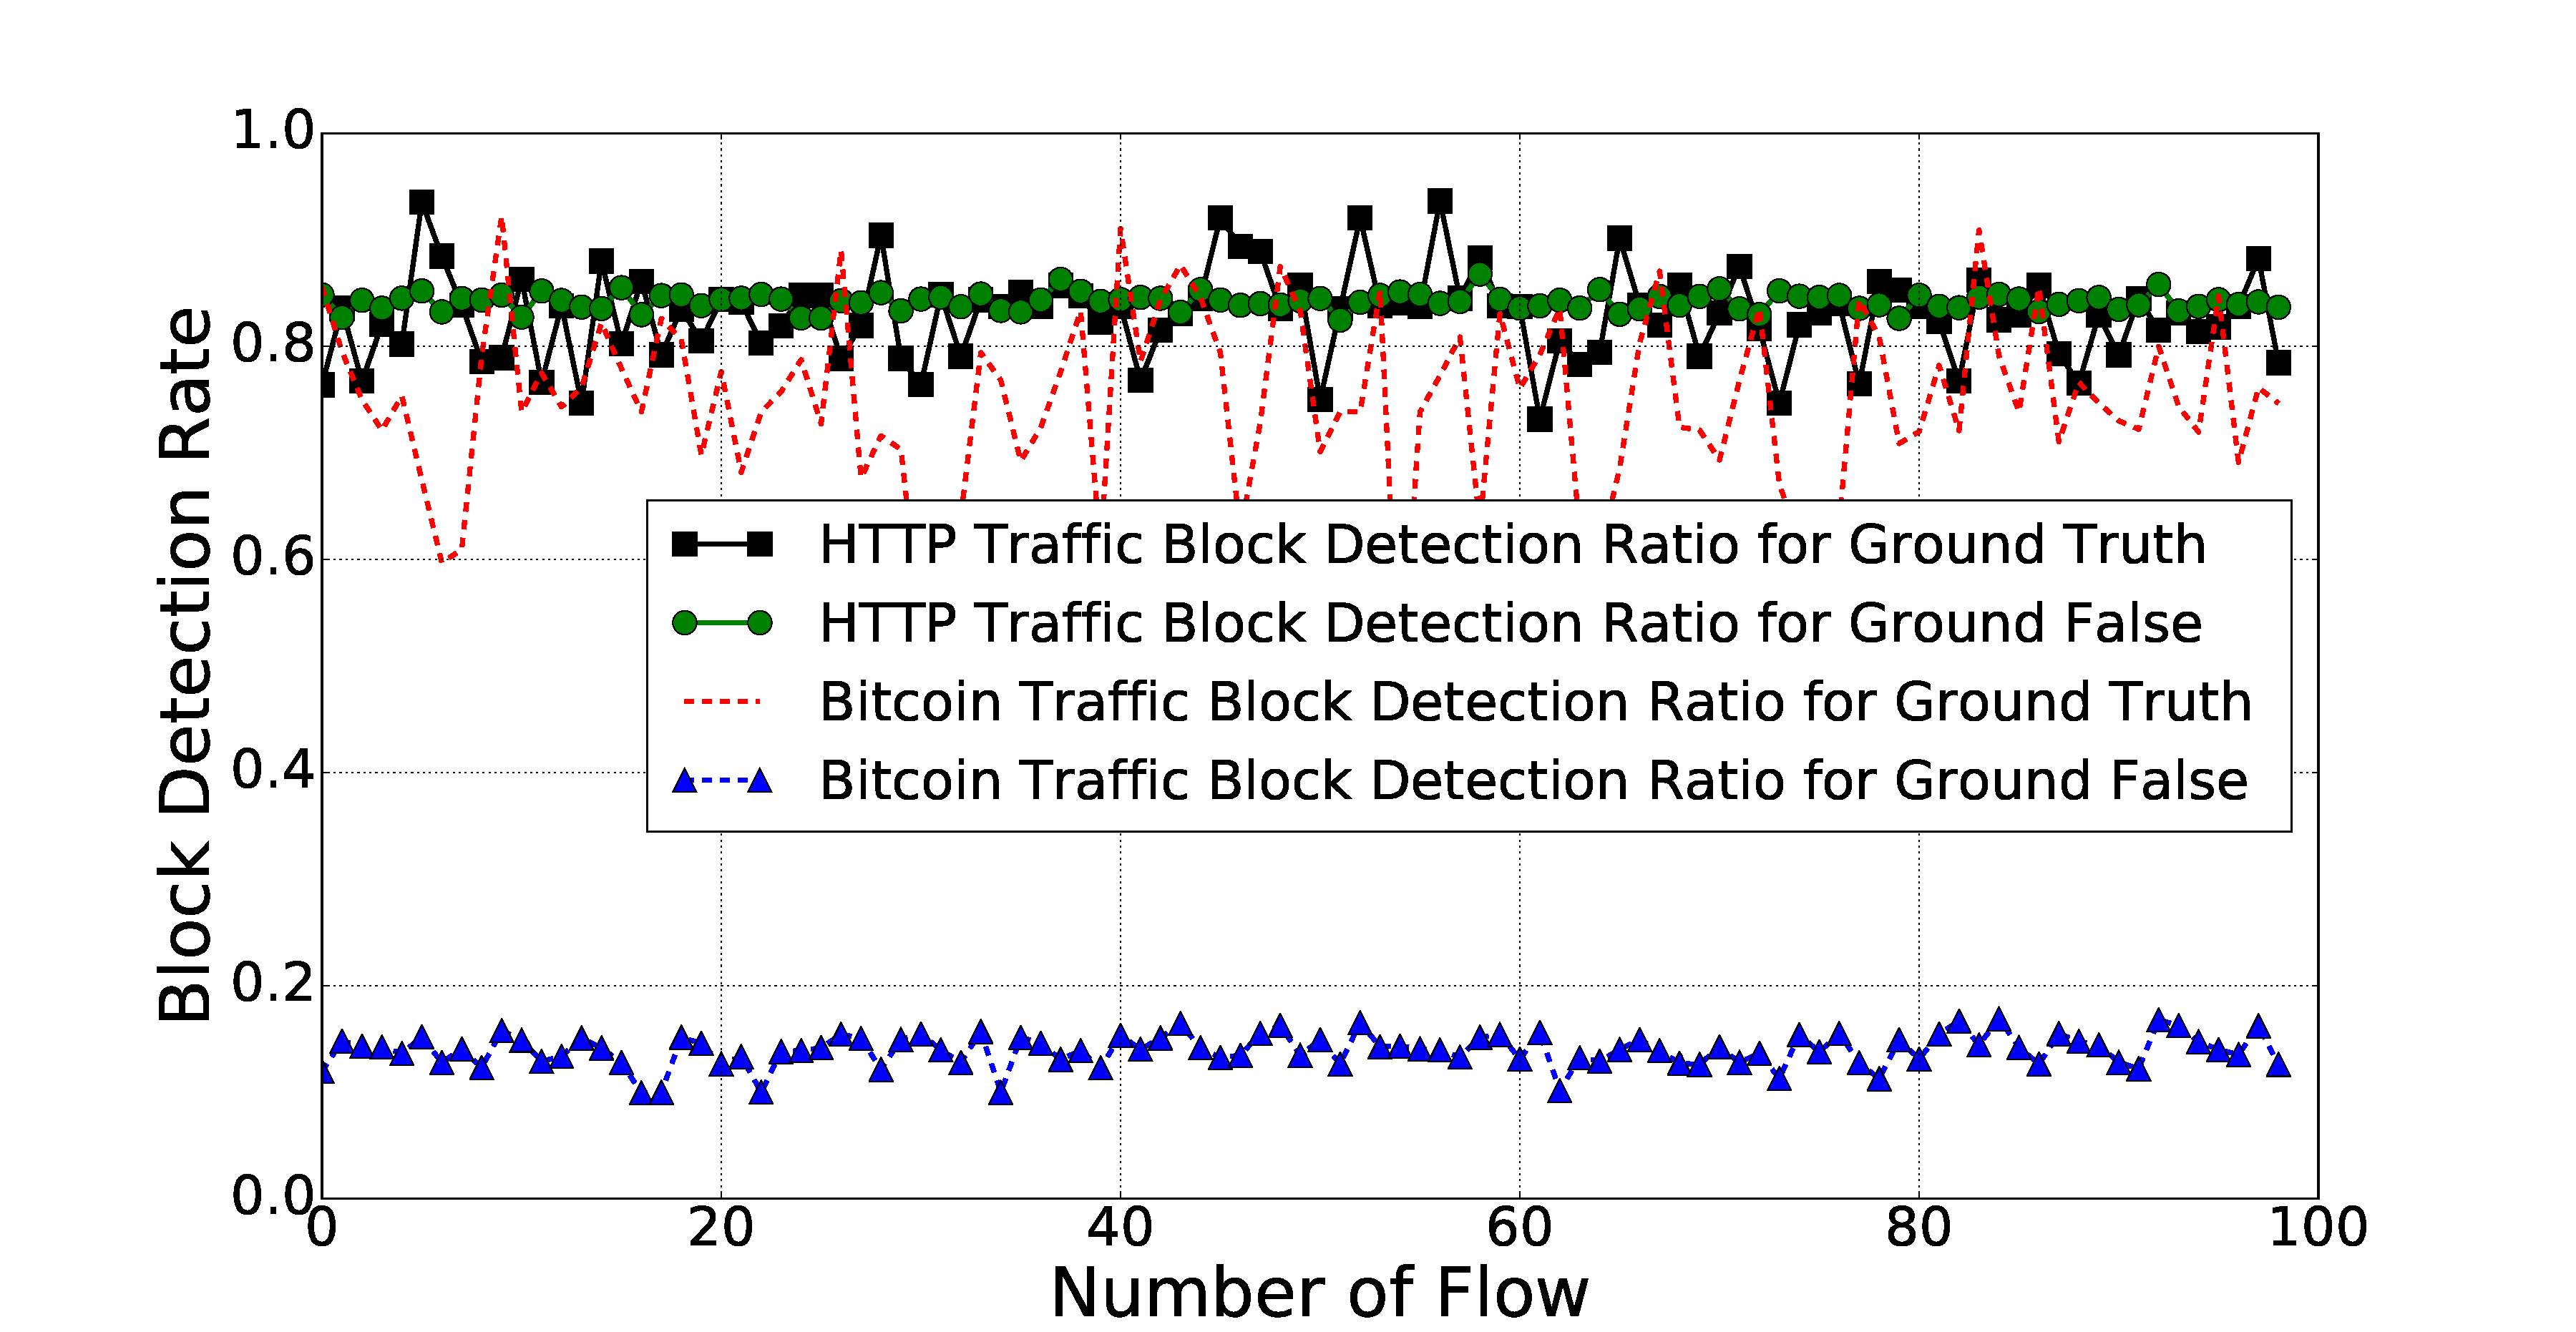
\includegraphics[width=\linewidth]{image/nov7/window/bc_http_window.pdf}
\caption{Detection Rate for Ground True and False}
\label{fig:gft_wind}
\end{subfigure}
\centering

\begin{subfigure}{\linewidth}
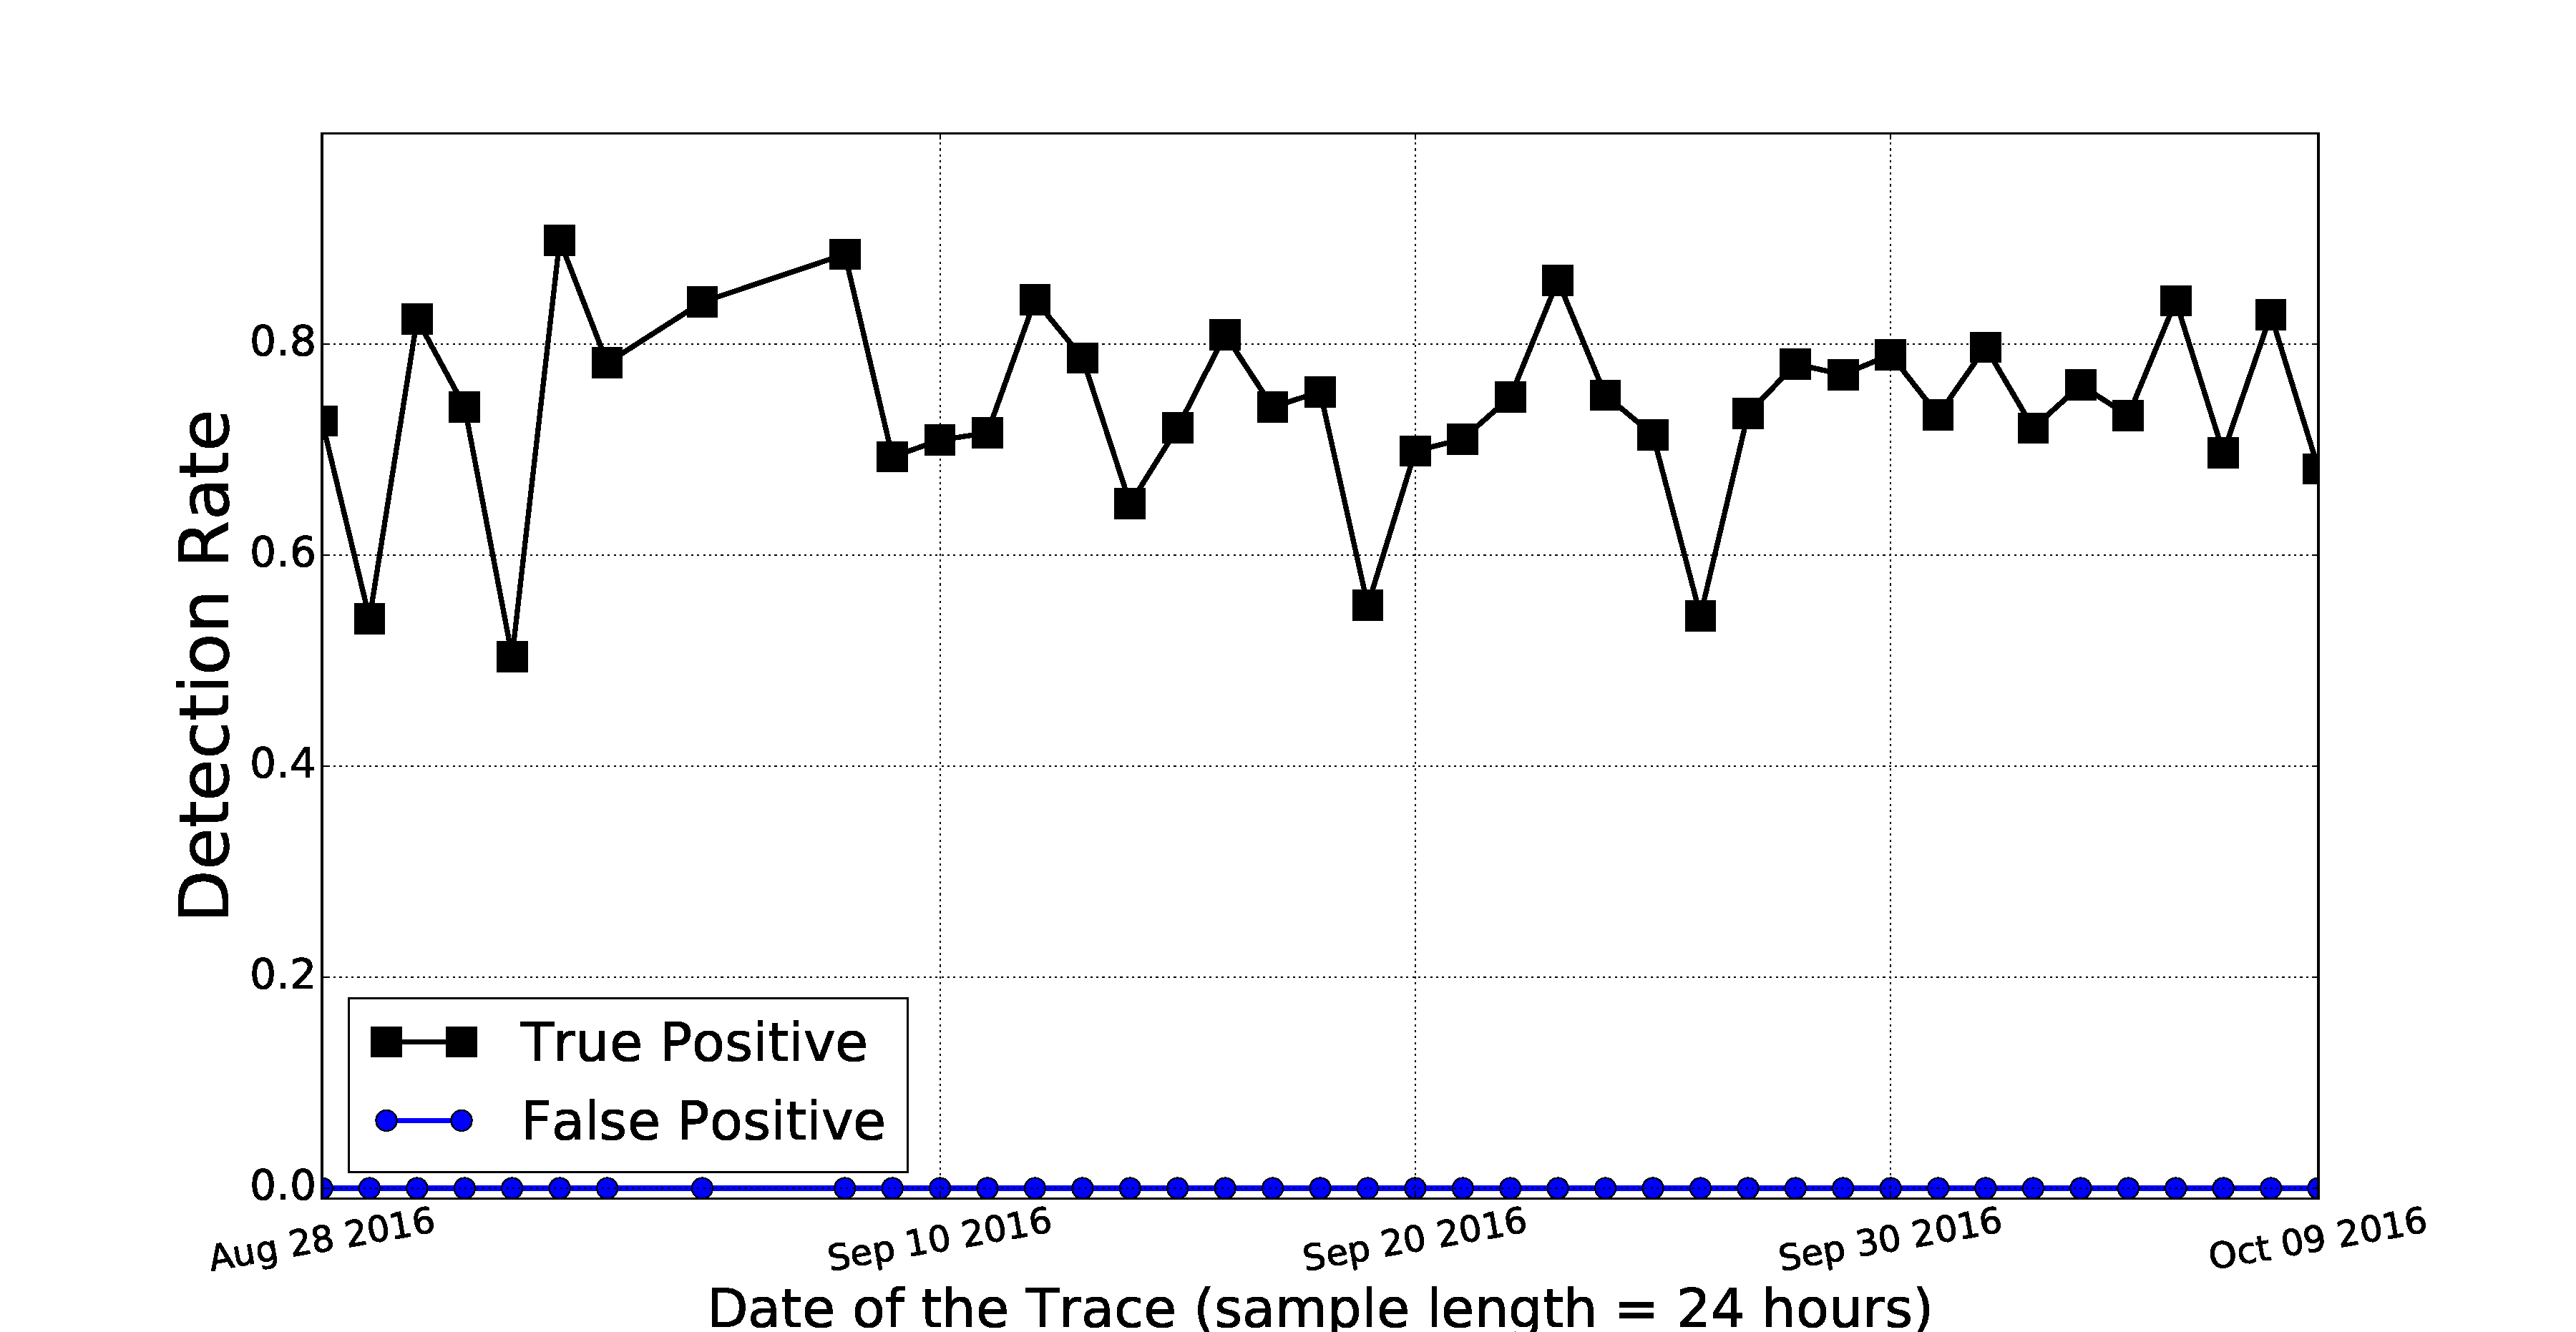
\includegraphics[width=\linewidth]{image/nov7/window/window.pdf}
%\caption{Result on full block mode}
\label{fig:res_wind}
\end{subfigure}
\caption{Window-based classifier}
\label{fig:window}
\end{figure}
\fi

\begin{comment}
 \begin{table}[h!]
  \begin{center}
    \caption{Traffic Class Breakdown For CAIDA Dataset}
    \label{tab:traffic_class}
    \begin{tabular}{c|c|c|c}
     \textbf{Traffic Class}& \textbf{Port Numbers} &\textbf{$\sharp$ of 			  Connections}&\textbf{$\%$of Total}\\
      \hline
		http, https& $80, 8080, 443$&745262&$0.318$\\
		dns& $53$&1073758&$0.457$\\
		smtp& $25$&2646&$0.001$\\
		telnet&$23$&6958&$0.003$\\
		ssh/scp&$22$&4928&$0.002$\\
		other&$-$&511700&$0.219$\\
		\hline
		all &&2345252&1.0\\
		\hline
    \end{tabular}
  \end{center}
\end{table}
\end{comment}

\begin{table}
\center \caption{Traffic class breakdown for CAIDA dataset}\label{tab:traffic_class}
\begin{tabular}{|c|c|c|c|}
\hline
 Traffic class& Port numbers &Number of connections&$\%$of total\\
      \hline
		http, https& $80, 8080, 443$&745262&$0.318$\\
		dns& $53$&1073758&$0.457$\\
		smtp& $25$&2646&$0.001$\\
		telnet&$23$&6958&$0.003$\\
		ssh/scp&$22$&4928&$0.002$\\
		other&$-$&511700&$0.219$\\
		all &$-$&2345252&1.0\\
\hline
\end{tabular}
\end{table}

\subsection{Metrics}

We use following metrics to measure the performance of our classifiers:
\begin{compactitem}
\item \textbf{True positive:} True positive shows the proportion of the data which contain \bc, and our model correctly identified as \bc traffic.
\item \textbf{False positive:} False positive shows the proportion of the data which did  not contain \bc traffic, and our model incorrectly classified as \bc.
\item \textbf{Accuracy:} Accuracy shows the proportion of the data which was correctly classified.
\end{compactitem}
\begin{figure*}

\begin{subfigure}{0.48\linewidth}
\centering
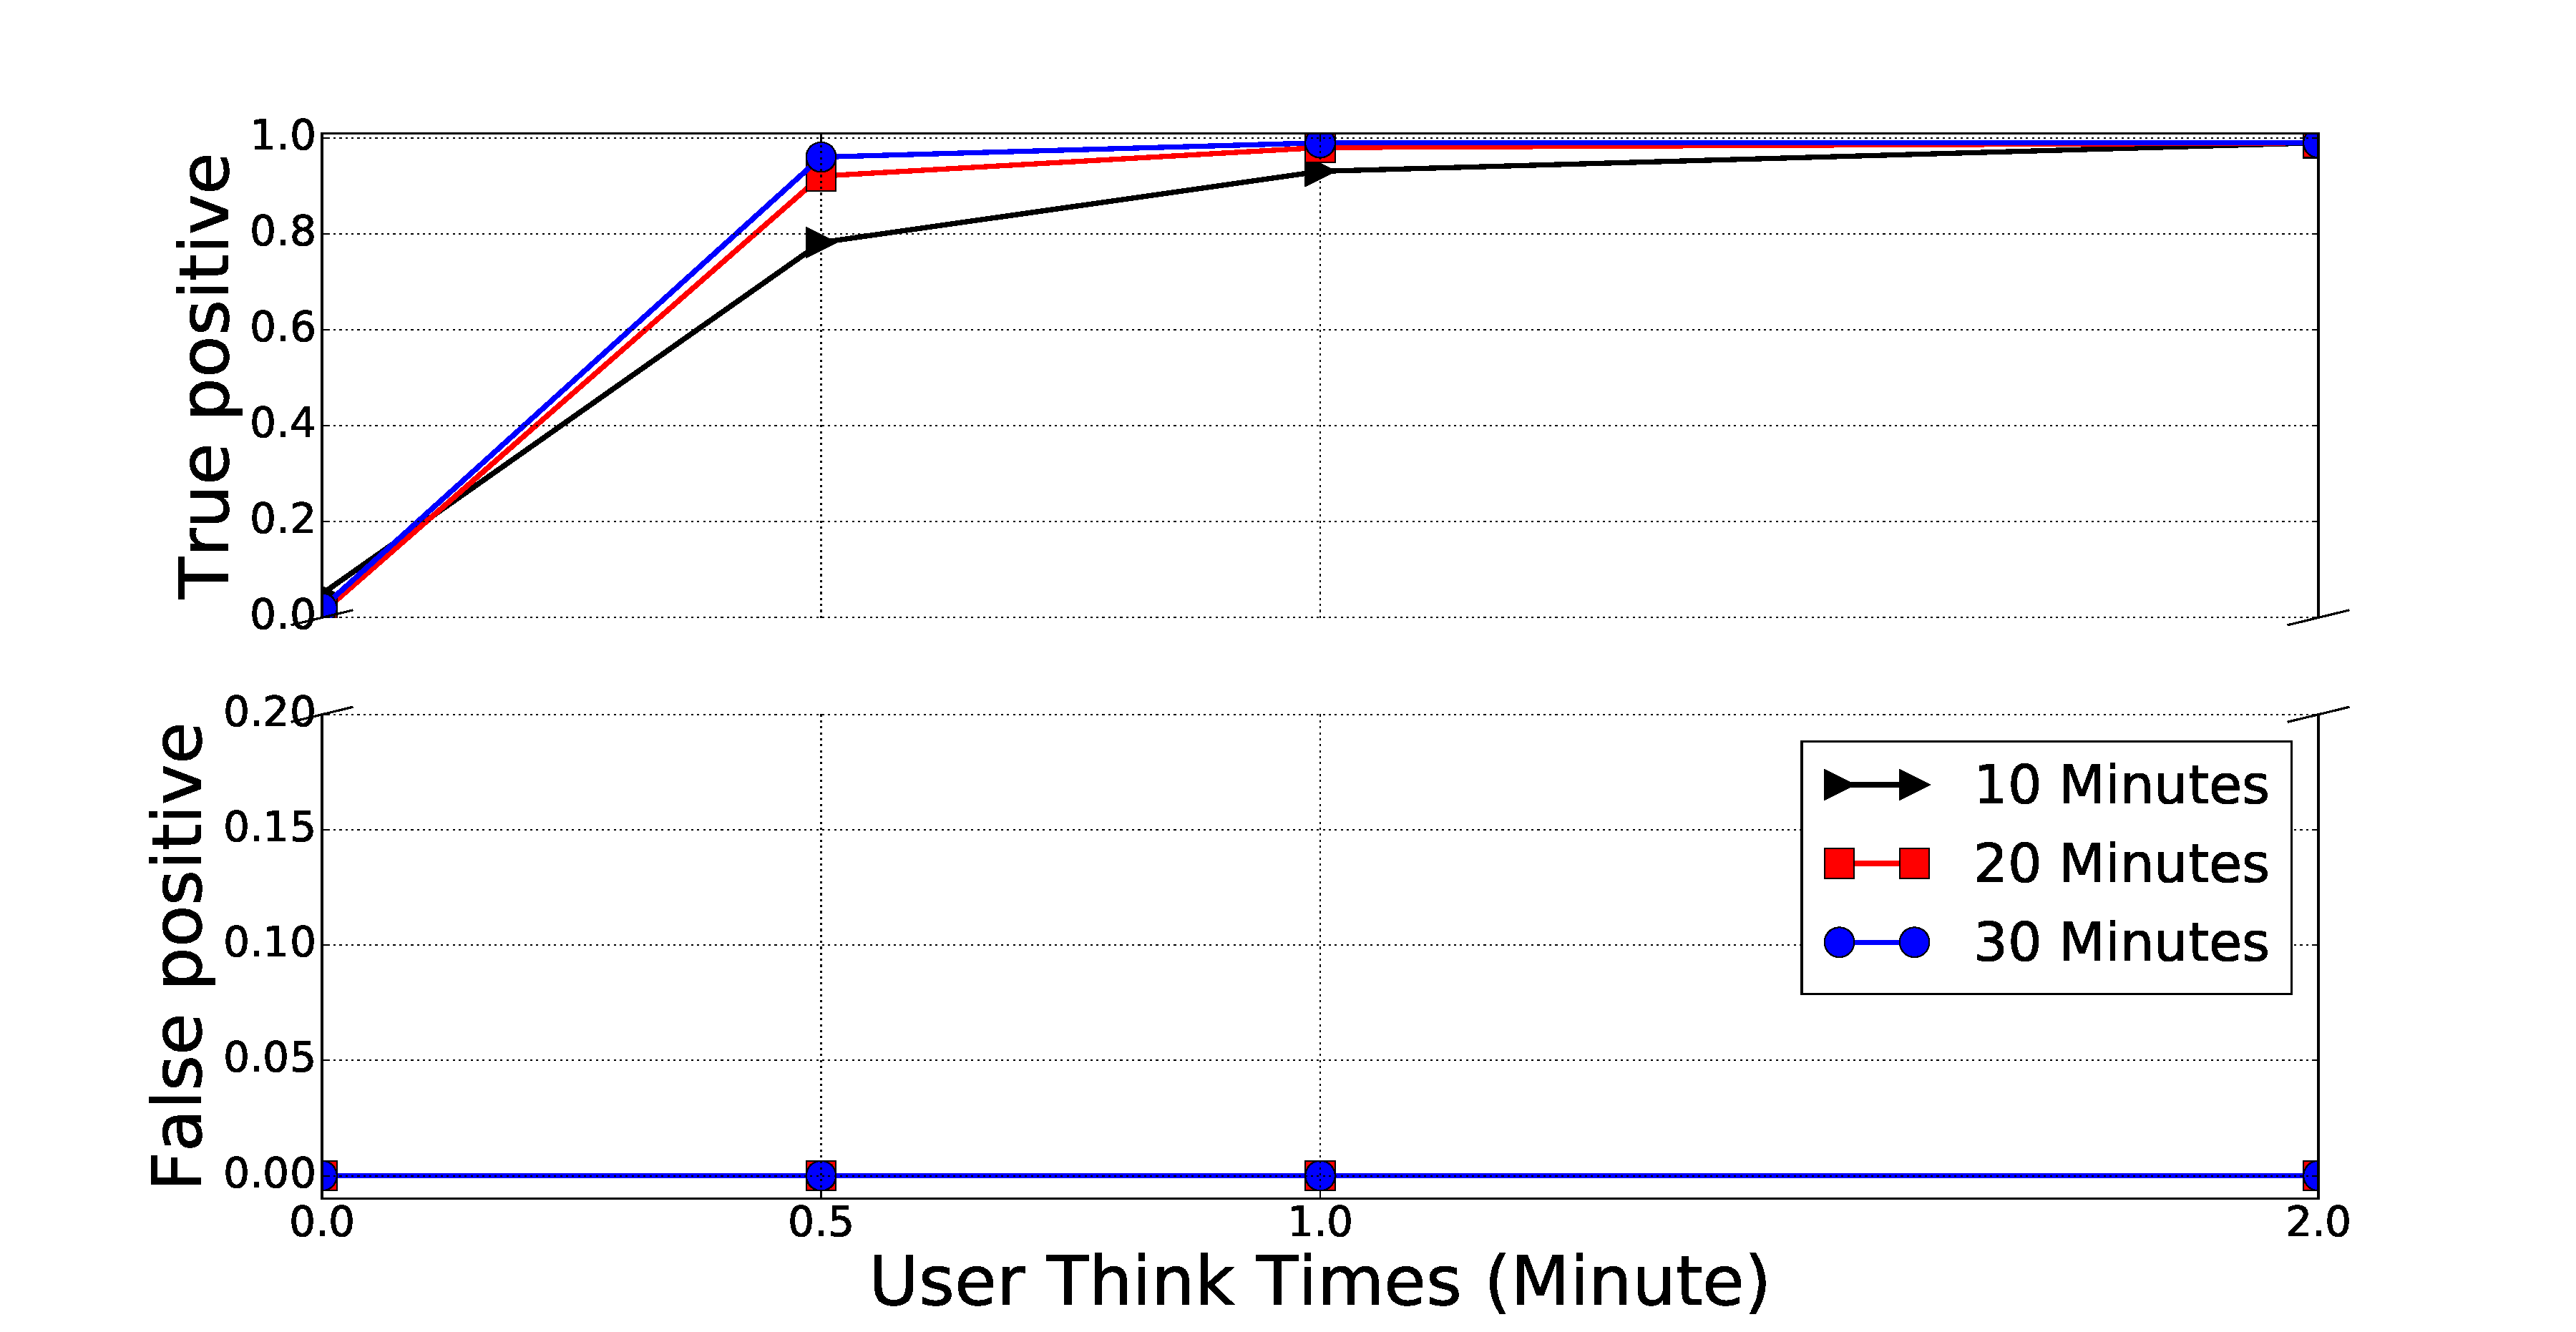
\includegraphics[width=\linewidth]{image/jan25/cmp_sizeHist.pdf}
\caption{Compact Mode}
\label{fig:vanilla_sizeTor}
\end{subfigure}
\begin{subfigure}{0.48\linewidth}
\centering
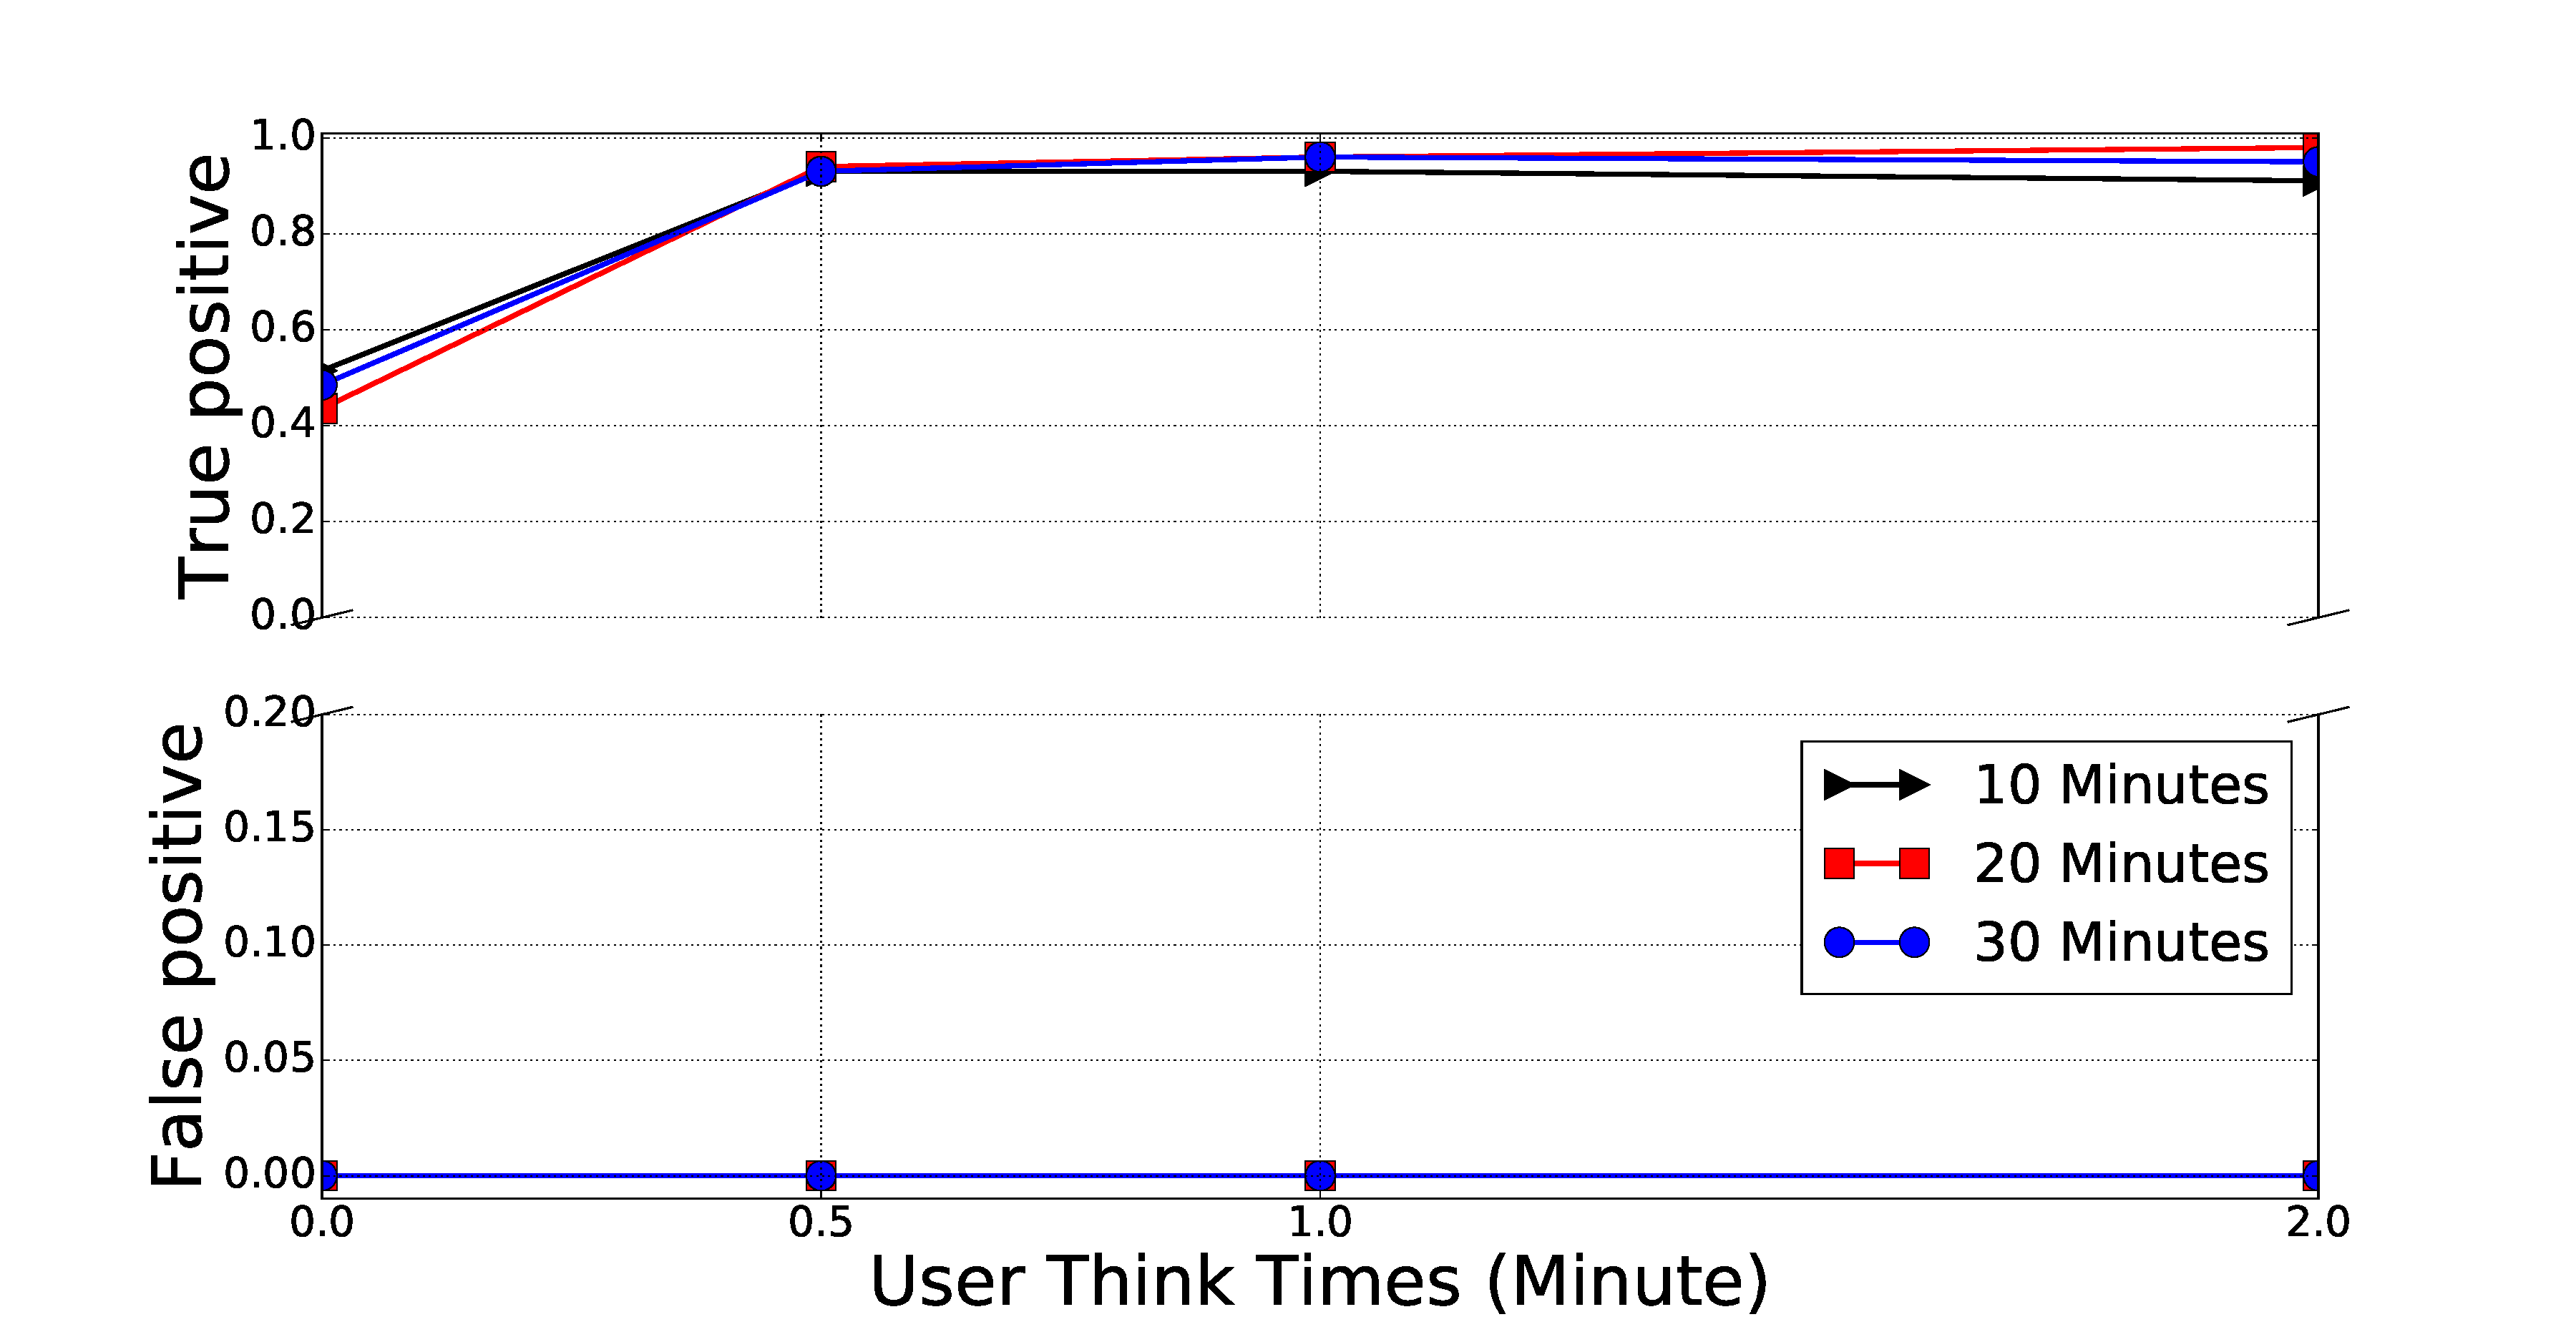
\includegraphics[width=\linewidth]{image/jan25/full_sizeHist.pdf}
\caption{Full Mode}
\label{fig:vanilla_d2u}
\end{subfigure}
\caption{Result of \code{sizeHist} classifier on noisy Bitcoin traffic}
\label{fig:sizeHist_non}
\end{figure*} 
\subsection{Modeling Normal Users}\label{simpleuser}

In this section, we describe four different types of users' profile that we use to evaluate the performance of our \bc classifiers against.% Users may have some background traffic while using Bitcoin or they can generate noisy traffic to evade detection. Therefore, we attempt to model typical behavior of users in various scenarios, and apply each classifier on one or more number of these profiles to evaluate their performance.

\begin{itemize}
    \item Simple User: A simple user is a Bitcoin client with no background noise and traffic. This type of user does not generate any network traffic except the Bitcoin client application traffic. Therefore, all traffic of the simple user is Bitcoin traffic. 
    \item Simple Noisy User: A simple noise user is a \bc client who browses only \textbf{one} webpage.% In some cases, she may run the Bitcoin client as well. 
    To control the background traffic, we introduce a parameter named think time, T, representing the amount of time that the user spends on a particular website. %Note that, increasing T would decrease the background noise since there is not much traffic after a website is loaded. Thus, if T is large and the Bitcoin application is running, after the webpage is completely loaded, the simple noisy user's traffic would look like the simple user's traffic.
    \item Complex Web (Complicated/Sophisticated) User: A complex user is a \bc client who browses \textbf{multiple} websites simultaneously.
    
     %Similar to the simple noisy user, she may run the Bitcoin application besides web surfing.% The user has the ability to use Tor to hide all of her traffic consisting of the Bitcoin and web traffic but she may decide not to use Tor. Thus, she can choose to pass all or none of her traffic over Tor and not some of it. 

\begin{comment}
    The complex web user is the sophisticated version of the simple noisy user. 

To create a sample data of this user profile, we choose a \bc traffic with length of sample size and accumulate the noise traffic using following algorithm: 
\begin{enumerate}
 \item Choose a random number ($k$) in the range $[0$, \textit{sample size}$]$, which represents
 the length of noise flow. 
 \item  Choose another random number ($p$) in the range $[0$,  \textit{sample size}$ - k]$, which shows where we
 need to add the noise: p's second of the \bc traffic.
 \item Repeat 1.
\end{enumerate}
We repeat this process for $I$ number of times, which represents the number of open tabs. The reason that we do not add noise from start to the end of the flow is that we want to make the background noise nonuniform, thus prevent the classifier from learning the noise and denoising the traffic.\end{comment}
    \item Complex CAIDA User: A complex CAIDA user is a \bc client who is running 1-5 number of CAIDA applications, which is introduced in table 2 simultaneously in the background. %We use the same algorithm as above to create this user profile.
\end{itemize}    
%We define four different user profiles from simple behavior to more realistic and complicated ones. 


\begin{comment}

In this section, we describe the type of users that we use to evaluate the performance of our \bc classifiers.
\subsubsection{User profiles for SizeHist and D2U classifiers}\label{binary_user_noise}
We consider two user profiles to evaluate the performance of our \bc classifiers in simple scenarios. First scenario is a \bc user who has no background noise. 
\begin{compactitem}
\item Simple User: A \bc client with no background noise.
\item Noisy User: A \bc user who is browsing Internet on the background. To control the background traffic, we introduce a parameter named \textit{think time}, T, which represents a time that user spends on a particular website. Note that, increasing T would decrease the background noise Since there is not much traffic after a website is loaded.
\end{compactitem}


\subsubsection{User model for NN-based and SizeTor classifiers}\label{setup:nn}
Here, we expand the user profiles in the previous section to have a more realistic scenario to evaluate our NN-based and SizeTor classifiers.%We generate a large corpus of data consisting of a user with $2-5$ number of open tabs. Also, a user who is running one or more number of applications -introduced in table~\ref{tab:traffic_class}- at the same type.

\begin{compactitem}

\item Complex User-1: A user who is browsing the Internet and browses multiple websites simultaneously. To create this user profile, we accumulate traffic from different websites. For example, for a background noise of two tabs, we add the traffic of two different websites.

\iffalse and has $2-5$ number of open tabs (she can be a \bc client as well). Since this model represents a user with
larger background noise, we consider $T$ to be $0$ seconds. Note that each open tab represents a single layer of background noise. We create each layer of background noise using the following algorithm:
\fi
 

 \item Complex User-2: A user who is running $1-5$ number of applications simultaneously, which is introduced in table ~\ref{tab:traffic_class} (she can also be a \bc client). 
\end{compactitem}
Therefore, we have $4$ type of users: complex User-1 with and without \bc, and complex User-2 with and without \bc. We add these user types to the previous ones to create a big corpus of data for our NN-based and SizeTor classifiers.
\end{comment}

\vspace{-0.2mm}
\section{Results}\label{sec:exp}
In this section, we implement our classifiers to evaluate their performance on user profiles described in part~\ref{simpleuser} writing more than a thousands lines of code in Python. First, for each classifier, we declare the user profile(s) that we use for evaluation of its performance and the false data that we use for computing its false positive. Second, we describe the result of each classifier and give a summary and comparison of them at the end of this section. 

\subsection{User Profiles and False Data}

For each classifier, we use a specific user profile and depending on that we choose the false data. As we explained above, false data is the base traffic that we use to compute false positive. Note that, we use same length of traffic for \bc and the false data. In other words, it is the traffic that we compare our \bc traffic with. For example, when we have 10 minutes of HTTP traffic, we are continuously browsing different websites for 10 minutes. We make these samples by concatenating the browsing of different websites.
 In the following, we describe these pairs for each classifier(s). 
\begin{compactitem}

\item For shape-based classifier, we use the simple user profile. Furthermore, we use HTTP which is the typical user behavior as the false data. This experiment evaluates if \bc traffic can be differentiated from browsing an HTTP website. 
\item  For the rest of the binary classifiers in this section, we use simple noisy user profile and attempt to detect the presence of \bc. Note that, similar to the window-based classifier, we use HTTP for the false data. This experiment attempts to evaluate if browsing an HTTP website is enough to hide the \bc traffic. 
\item For the neural network-based and combined classifiers, we use the complex web and complex CAIDA user for training and testing.
\end{compactitem}
Note that, for these two classifiers, we evaluate our model using $10,000$ number of test data, and report the false positive, true positive and accuracy. For rest of the classifiers, we use $500$ number of test data for evaluation. Also, the data is balanced, which means we have the same number of data for each category.

%\subsection{Shape-based Classifier}
\begin{comment}
 \begin{figure*}[!t]
\begin{subfigure}{.48\linewidth}
\centering
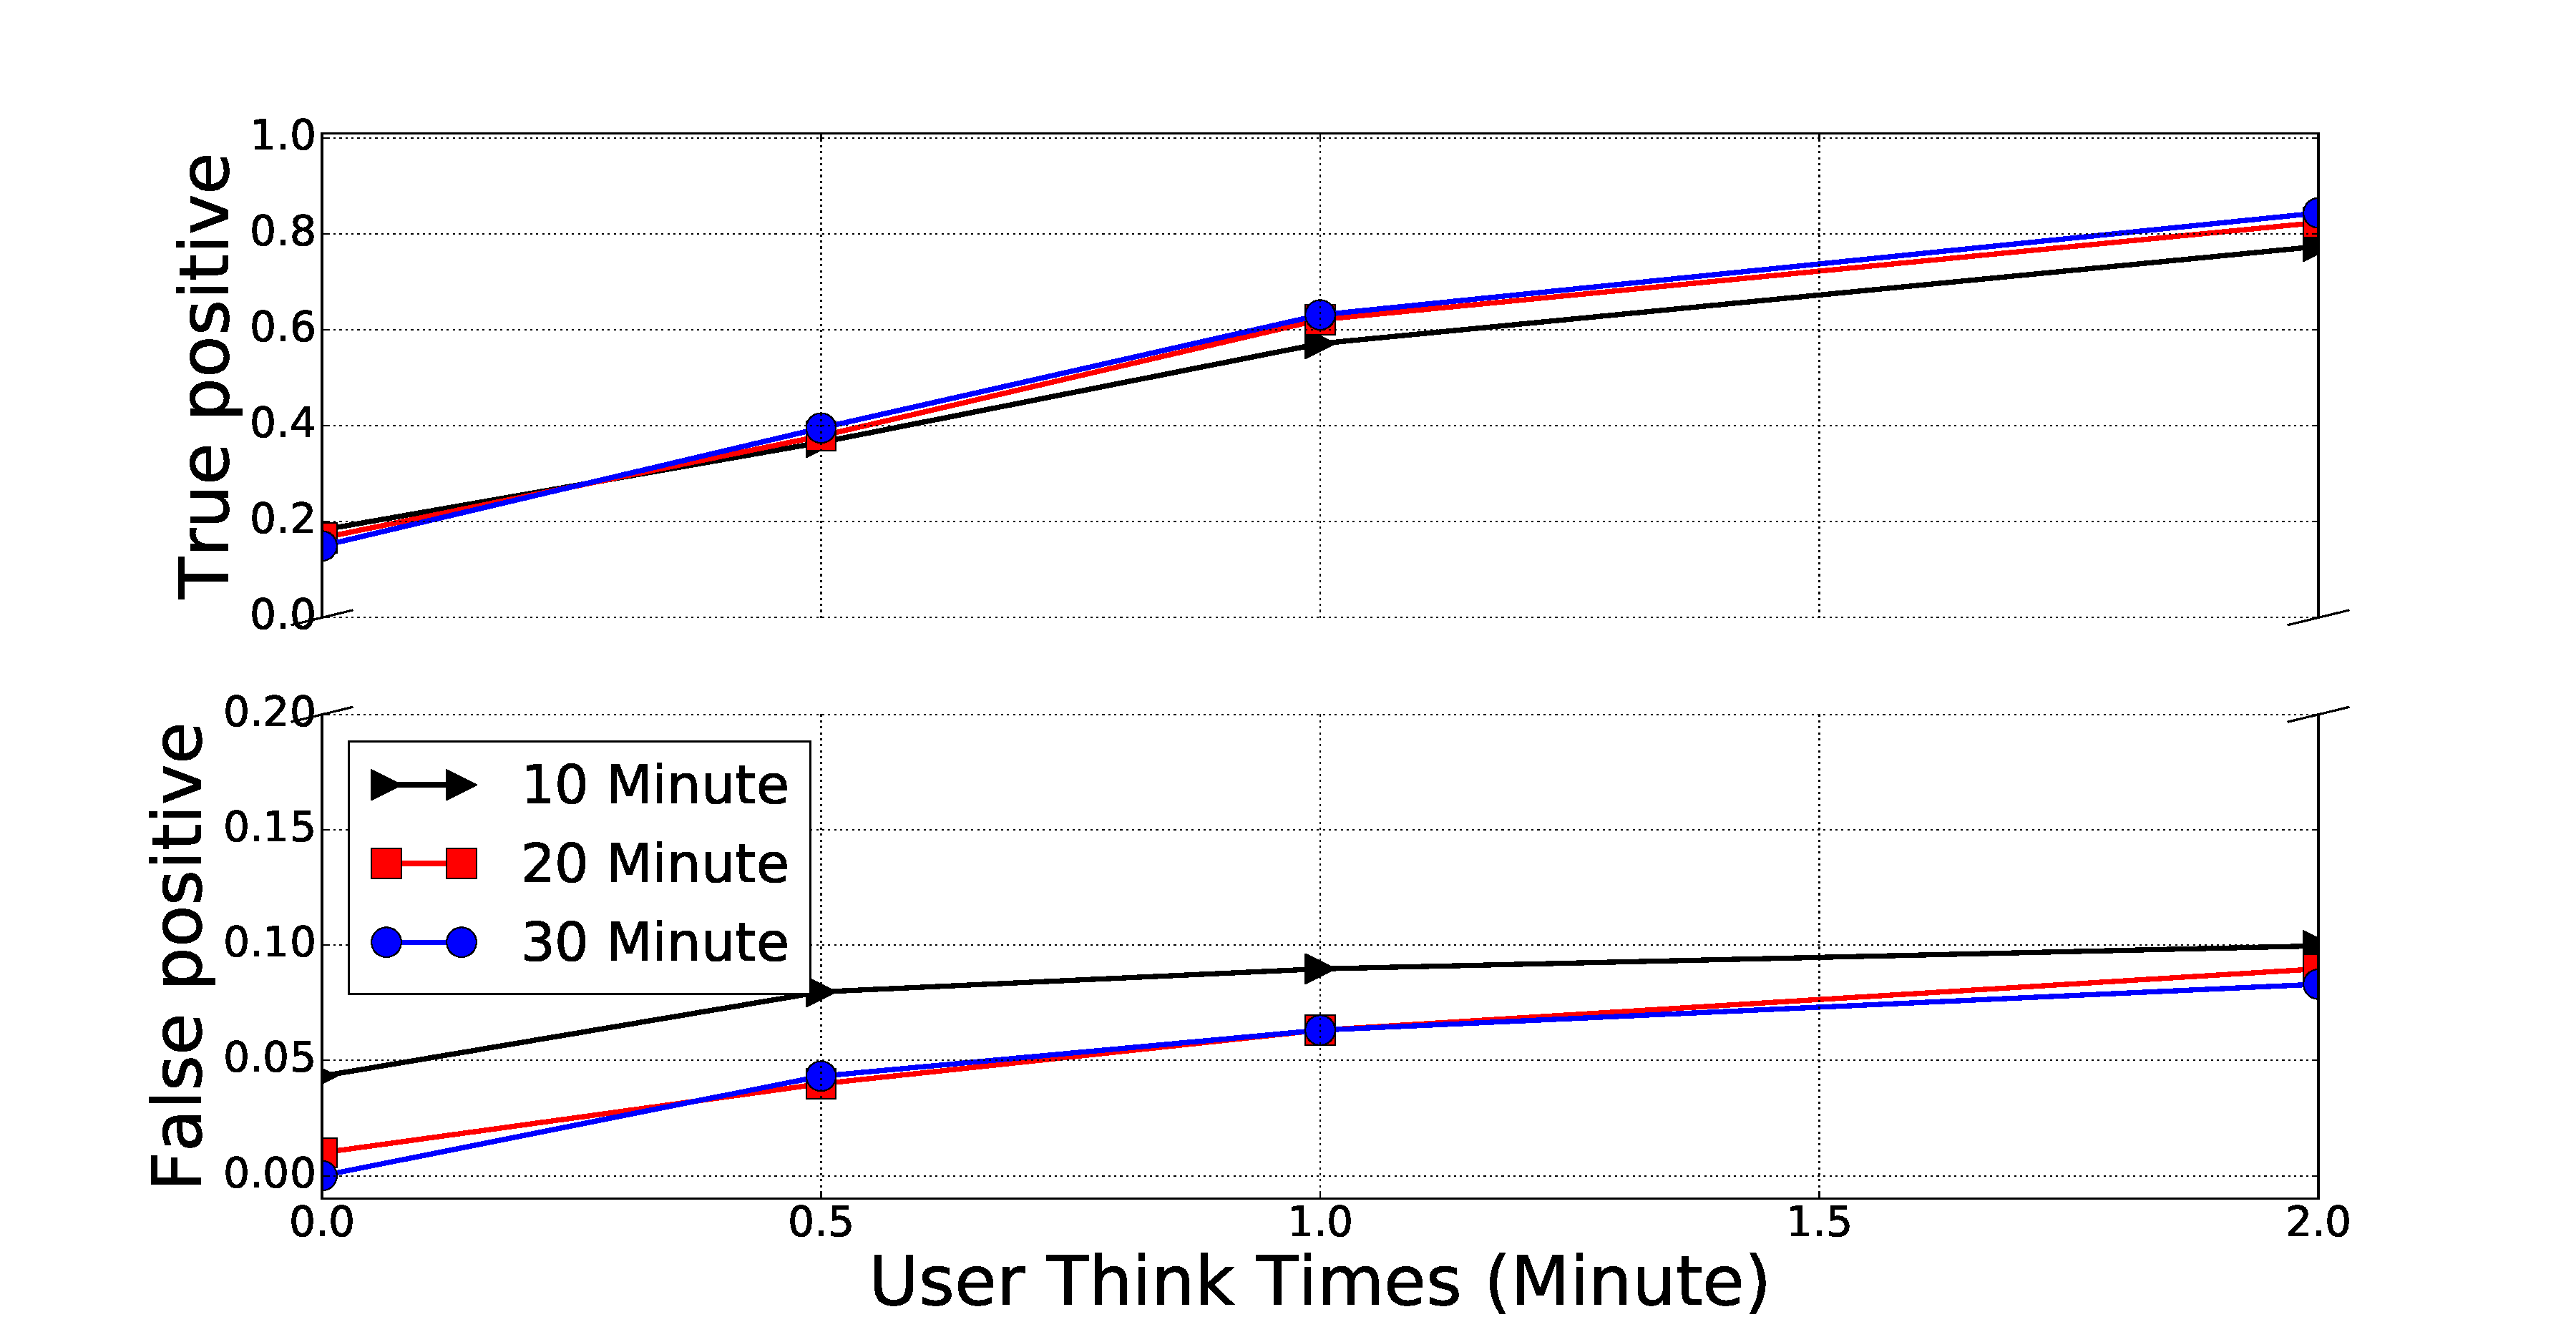
\includegraphics[width=\linewidth]{image/jan25/full_d2u.pdf}
\caption{Full Mode}
\label{fig:tp}
\end{subfigure}
\centering
\begin{subfigure}{.48\linewidth}
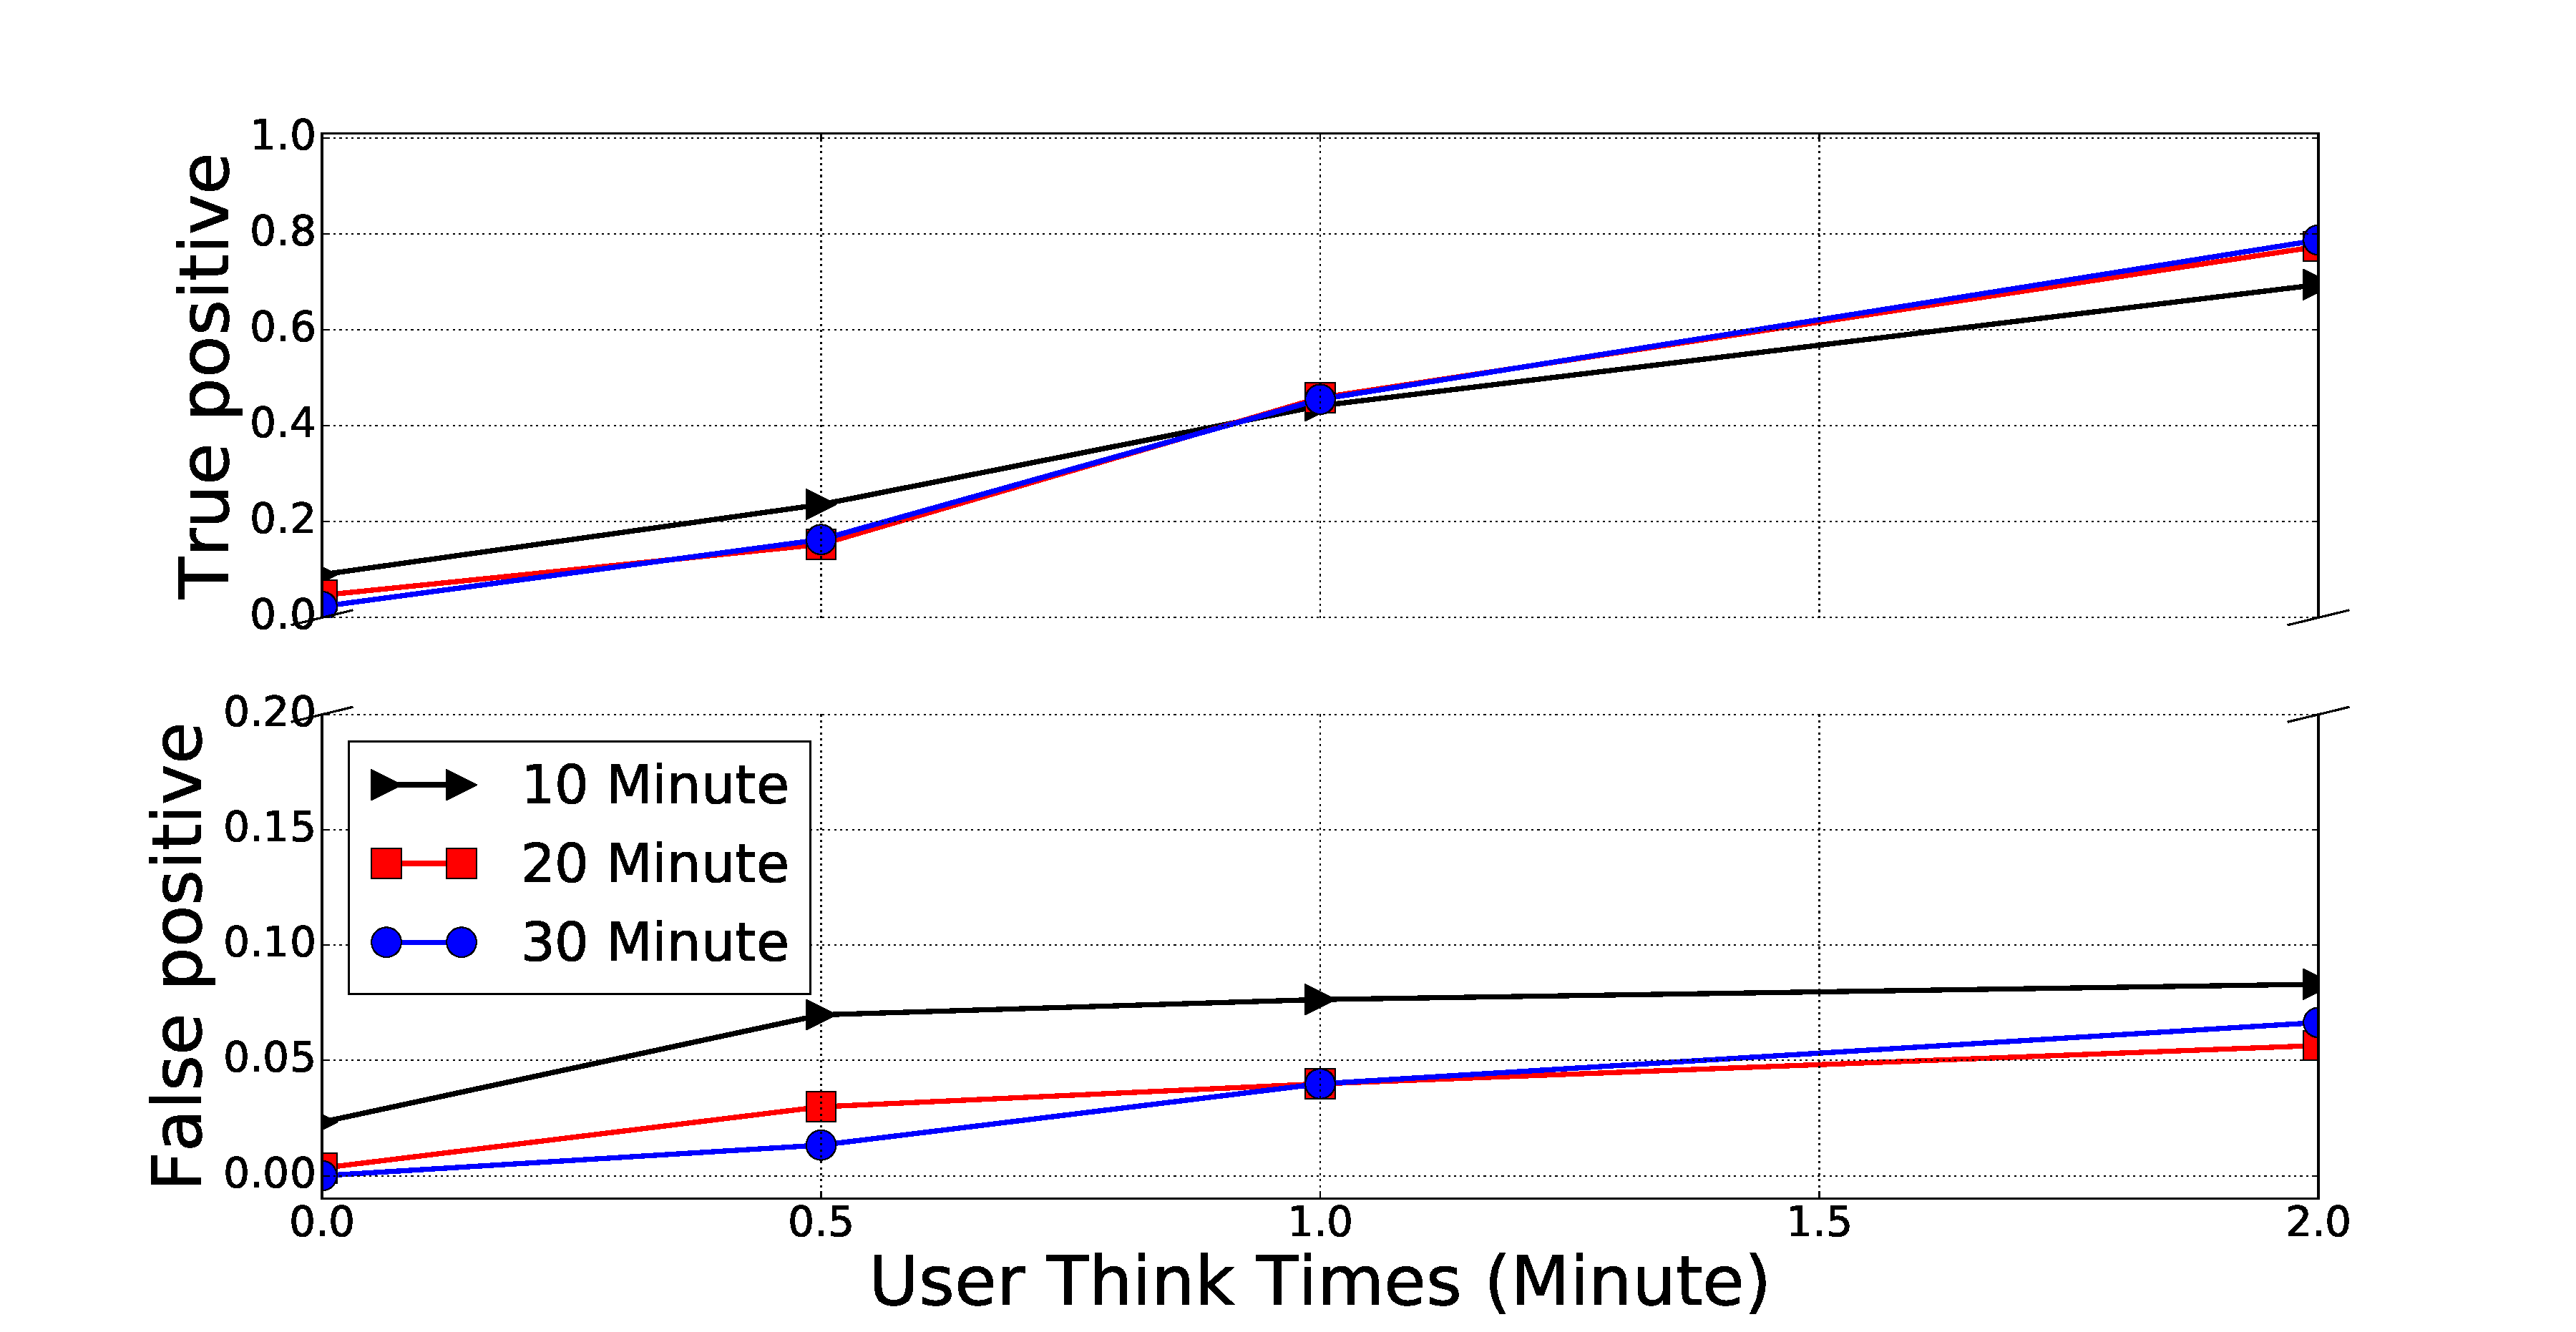
\includegraphics[width=\linewidth]{image/jan25/cmp_d2u.pdf}
\caption{Compact Mode}
\label{fig:fp}
\end{subfigure}
\caption{Result of \code{D2U} classifier on noisy \bc traffic}
\label{fig:d2u}
\end{figure*}
\end{comment}

\subsection{Size-based Classifiers}

\subsubsection{\code{SizeHist} Classifier}
%For this classifier, we compute the histogram of packet sizes and using a correlation algorithm we decide if the traffic contains \bc or not. Because of the \bc specific packet sizes, we expect to have a good performance even in the presence of background noise.
We implement the \code{sizeHist} classifier on \bc traffic in compact and full block modes using the noisy user model described in Section~\ref{simpleuser}. Figure~\ref{fig:sizeHist_non} shows the performance of this classifier. We control the noise using think time (T). Increasing T decreases the noise and enhances the classifier's performance. Figure~\ref{fig:sizeHist_non} shows that we can reach more than $90\%$ true positive and $0\%$ false positive for both modes when we have $10$ minutes of traffic and set T to $2$ minutes. It is worth stating that we could reach similar results when we set T to $0.5$ minutes and have $20$ minutes of traffic.

%impact of traffic length and background noise on true positive and false positive for this classifier. 
 
\begin{comment}
\subsubsection{The \code{D2U} Classifier}
We showed in Appendix~\ref{sec:charachterzing_bc} that downstream to upstream ratio of \bc traffic could be a distinguishing factor to identify \bc from other traffics. D2U classifier attempts to use the symmetry between upstream and downstream of \bc traffic to distinguish it from other protocols. Figure~\ref{fig:d2u} shows the result of this classifier on noisy user profile for full and compact block modes. It indicates that increasing T and thus decreasing the background noise on \bc traffic would improve the 
detection rate. More specifically, our true positive enhances from $0$ to $80\%$ when we increase T from $0$ to $2$ minutes.
\end{comment}


\subsection{Shape-based Classifier}
%As we explained in Section~\ref{window-sec}, shape-based classifier attempts to detect \bc blocks using the volume of traffic downloaded at a time window around the block announcements times, and using the block detection rate it computes the true and false positive.
To implement this classifier, we set $J$ and $\omega$ introduced in Section~\ref{window-sec} to $100$ kilobytes and $20$ seconds, respectively. 
To set $\eta$, we compute block detection rate for \bc using ground false shown in Figure~\ref{fig:window}. We need to set $\eta$ to be larger than all the detection rate values for \bc using ground false. Note that each point for \bc using ground false in the figure is the average for $25$ different ground falses. Using this figure, we set $\eta$ to $0.4$. Moreover, Figure~\ref{fig:window} shows the block detection rate for HTTP using ground truth and block detection rate for \bc using ground truth too. Using the $\eta$, we can detect all \bc traffic through (August 28 - October 5) as \bc. Also, we did not classify any of the HTTP traffic as \bc, which results in $0\%$ false positive. Furthermore, the performance of shape-based classifier quickly diminishes in the presence of a small HTTP background noise. Also, we fail to detect \bc traffic in compact mode because of small block sizes, which makes it impossible to distinguish them.

%since HTTP noise dominates the \bc traffic and destroys the results of the classifier. Furthermore, we implement the shape-based classifier on \bc compact mode and learn that this classifier fails to detect \bc traffic in this mode because of small block sizes, which makes it impossible to distinguish them.
%As we explained in Section~\ref{window-sec}, $\eta$ is the threshold that we use to differentiate \bc traffic: if the block detection rate is higher than $\eta$, we classify the traffic as \bc.
 
 %Using these parameters, we could reach $100\%$ true positive and $0\%$ false positive for more than one months of \bc dataset (August $28$ - October $9$, $2016$). 


\begin{figure}
\centering
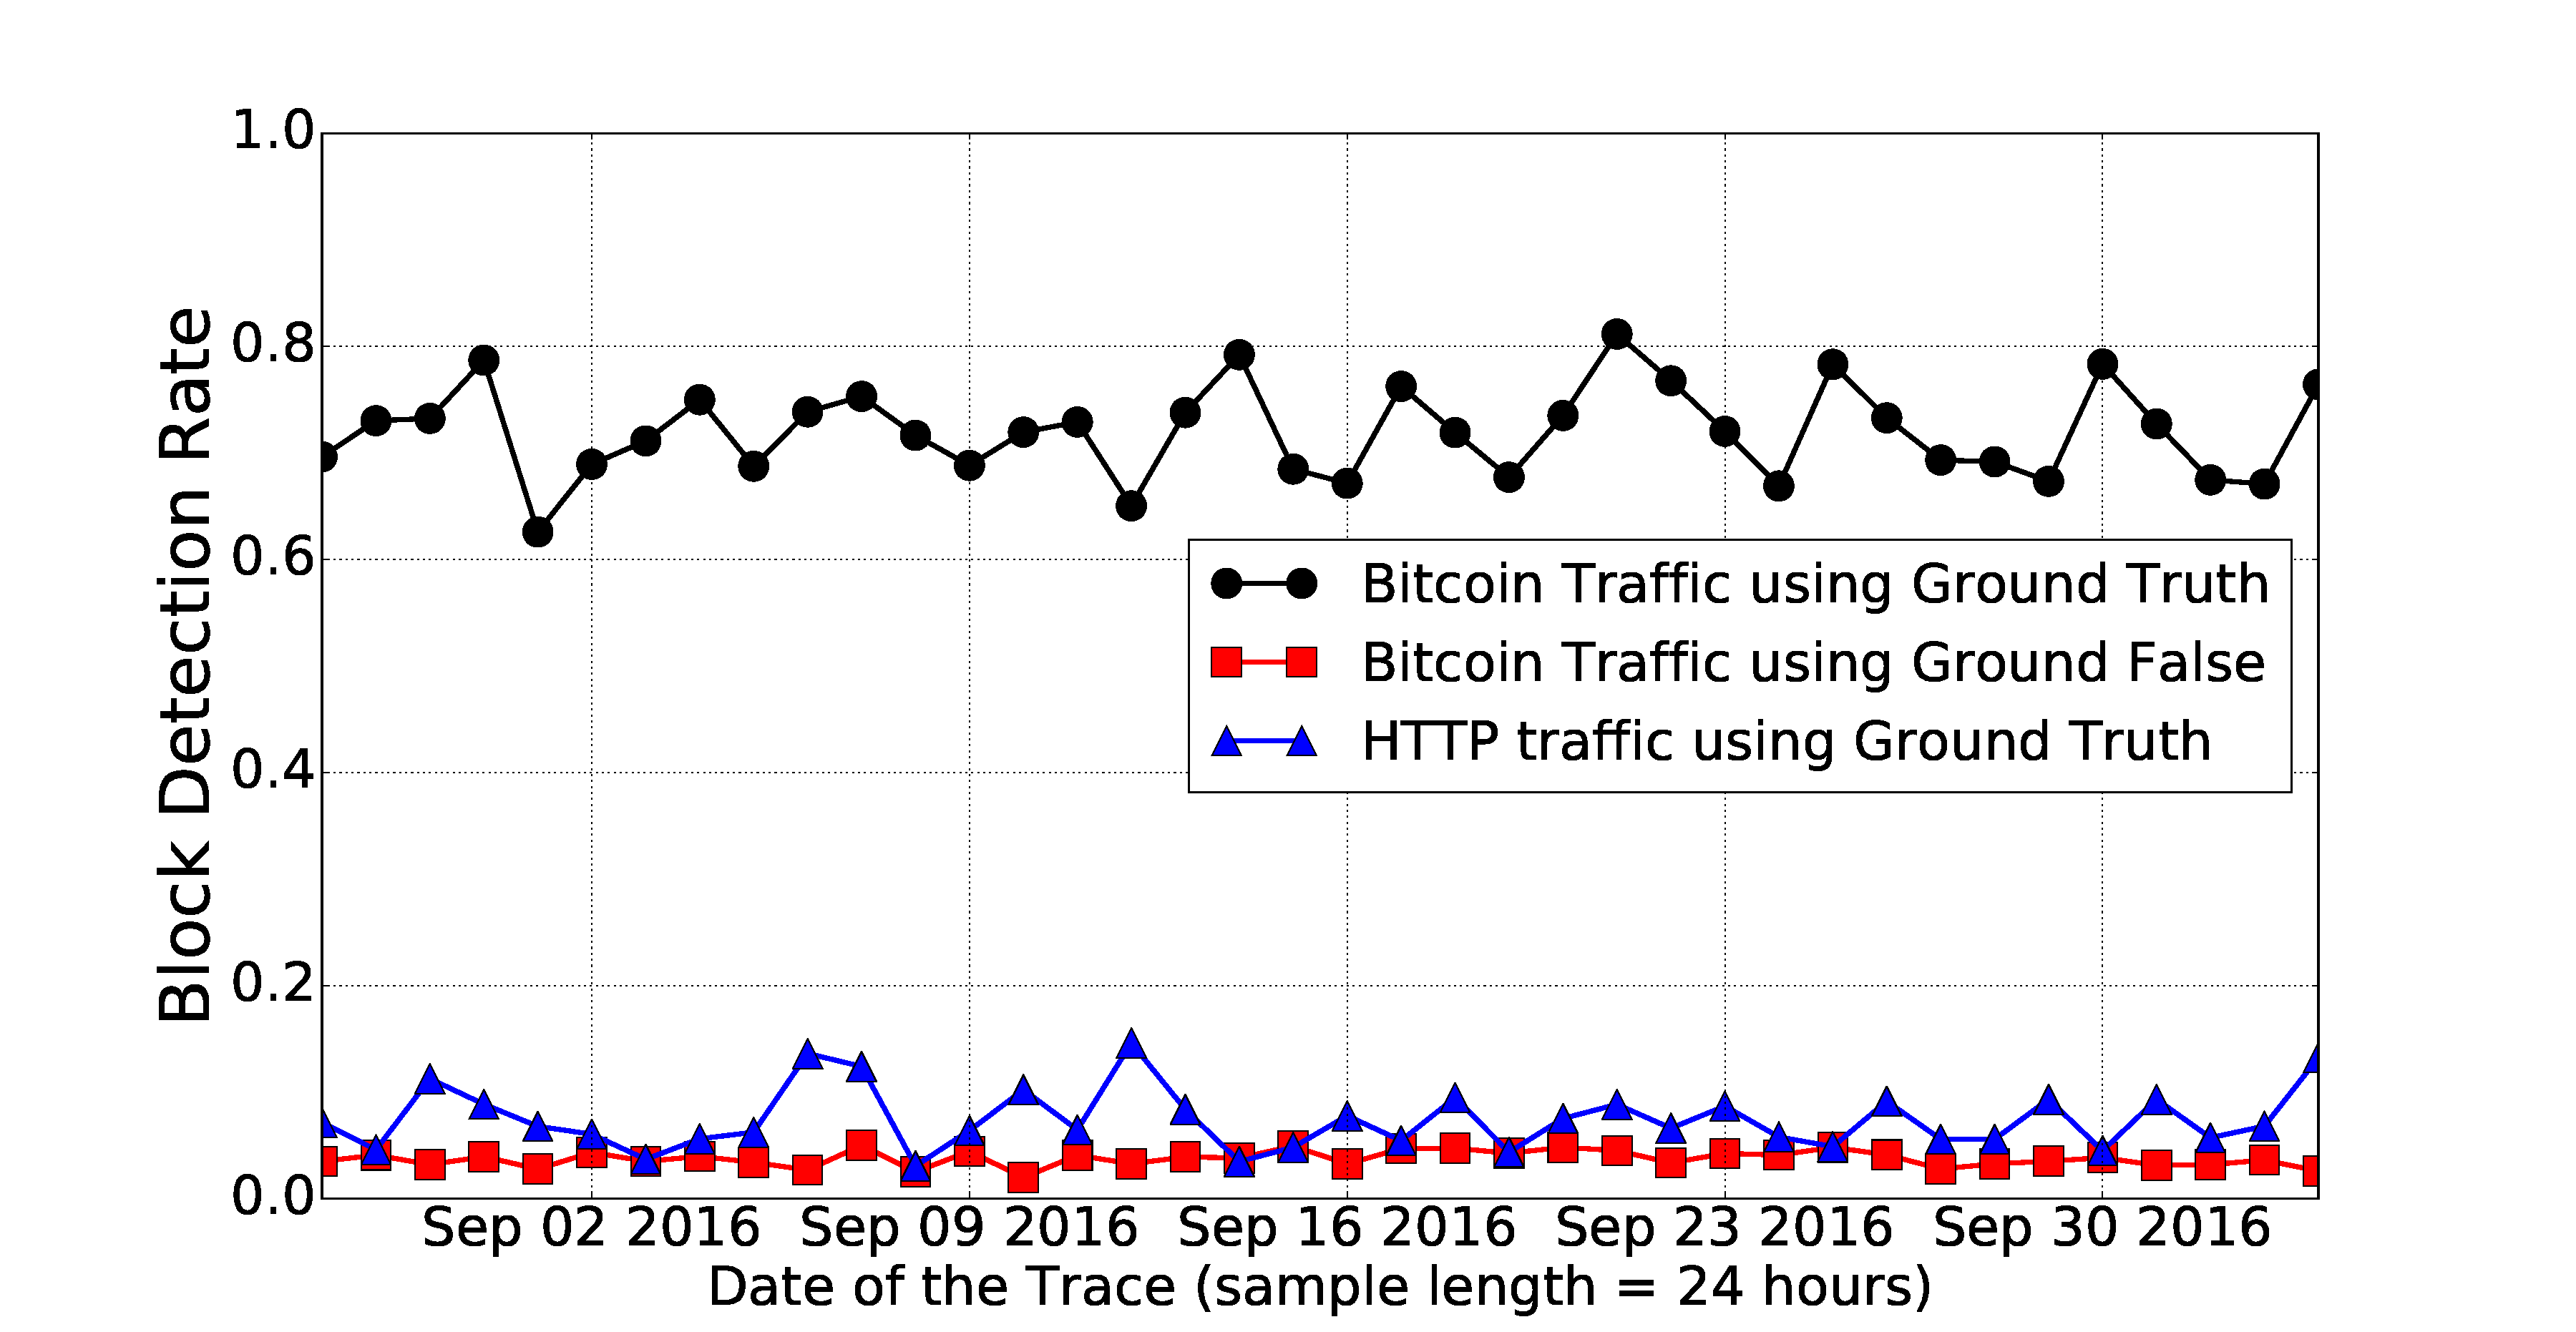
\includegraphics[scale=0.15]{image/jan25/window.pdf}%{image/nov7/window/window.pdf}%roc is also available%window_gf_gt_bitcoin.pdf
\caption{Block detection rate using shape-based classifier}
\label{fig:window}
\end{figure}
\subsection{Neural Network-based Classifier}

We implement the NN-based classifier using Keras~\cite{keras} with Tensorflow~\cite{tensorflow2015-whitepaper} backend. We use complex web and complex CAIDA user to evaluate its performance. Table~\ref{tab:nn} shows the result of NN-based classifier for different sizes of training data. As the table indicates, the accuracy of the classifier improves from $62\%$ to $96\%$ when we increase the size of training data from $1000$ to $40,000$. Note that, true and false positive improves from $44\%$ to $92\%$ and $20\%$ to $2\%$ respectively when we increase the size of training data.
\begin{comment}
To run this classifier, we need to set two parameters: learning rate and epochs.
 Learning rate is a hyper-parameter which controls how much we adjust the weights of the neural network model in each iteration. Moreover, epochs depict the number of times that the algorithm is run on the training data. We use the default value of $0.01$ for the learning rate of Adam optimizer ($lr$). For the epochs, we run our model for values ranging from $50$ to $2000$ and realize that using $1000$ number of epochs we can get a good performance from our classifier. Having a small value for epoch keeps the model from learning the dataset. On the other hand, having a very large number for it may cause over-fitting. Therefore, we need to pick this value very carefully. 
 
 
  Furthermore, increasing the number of epochs would increase the training time. For example, the training time increases from $20$ seconds to around $4$ minutes when we increase the number of epochs from $50$ to $1000$ for $5000$ number of training data. Therefore, we need to take this into account when the size of training data increases.
  \end{comment}
\begin{comment}
\begin{figure}
\centering
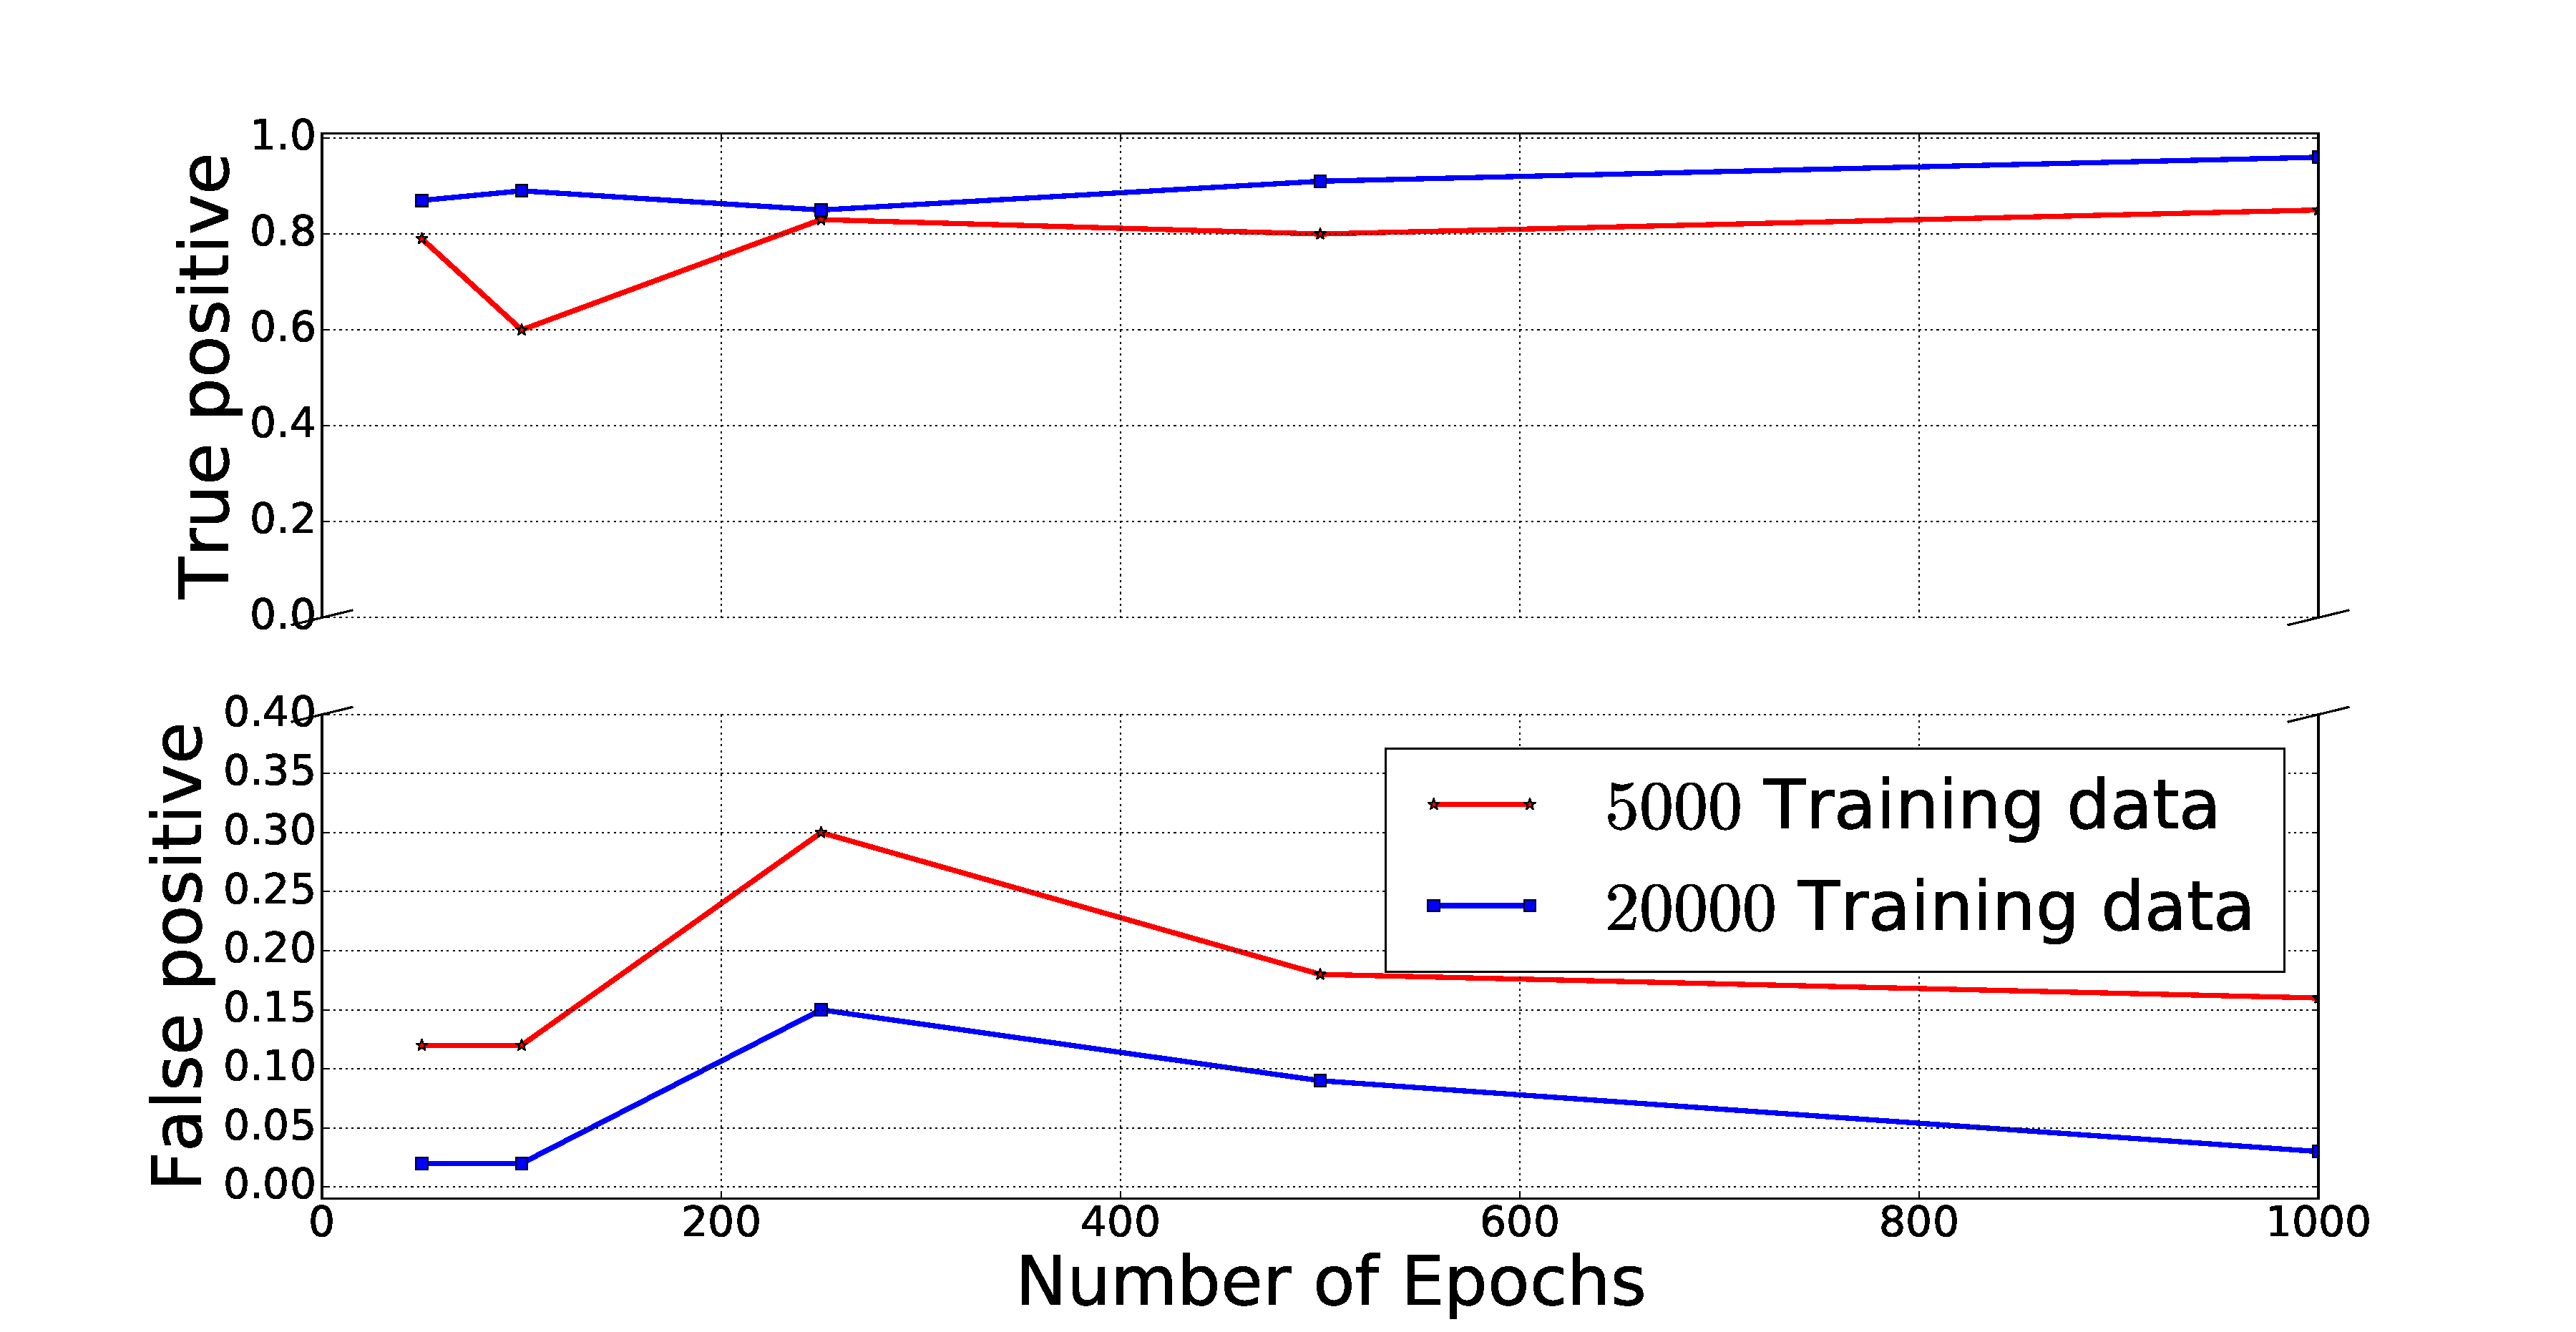
\includegraphics[width=\linewidth]{image/jan25/epochs.pdf}
\caption{Impact of Increasing the number of epochs in performance of the Neural Network Classifier}
\label{fig:epoch}
\end{figure}
\end{comment}

\begin{comment}
\begin{table}[h!]
  \begin{center}
     \caption{Result of Neural Network classifier}
    \label{tab:nn}
    \begin{tabular}{c|c|c|c}
    \kern 0.5pc \shortstack{ Training \\Size}& \shortstack{False Positive\\ ($\%$)} &\shortstack{True Positive\\ ($\%$)}&\shortstack{Accuracy \\($\%$)} \kern 0.5pc\\
      \hline
	$1000$&$20$ &$44 $  & $62$\\
	$5000$&$11$& $80$  & $85$\\
	$10,000$&$6$& $84$  &$ 89$\\
	$80,000$&$0.1$& $93$   & $96$\\% for 1000 epochs
    \end{tabular}
  \end{center}
\end{table}
\end{comment}

\begin{table}
\center \caption{Result of neural network classifier.}\label{tab:nn}
\begin{tabular}{|c|c|c|c|}
\hline
 Training size& False positive ($\%$) &True positive ($\%$)&Accuracy ($\%$)\\
      \hline
	$1000$&$20$ &$44 $  & $62$\\
	$5000$&$11$& $80$  & $85$\\
	$10,000$&$6$& $84$  &$ 89$\\
	$40,000$&$2$& $92$   & $95$\\% for 1000 epochs

	%$80,000$&$0.1$& $93$   & $96$\\% for 1000 epochs
\hline
\end{tabular}
\end{table}



\subsection{Combined Classifier}
To extend the neural network-based classifier, we defined combined classifier, which uses all of the attributes used in previous classifiers. Using this classifier, we reach $99.84\%$ accuracy with false positive of $0$ and true positive of $99.74\%$ having $40,000$ of training data and sample size of $10$ minutes. This result is very promising and shows that having enough data and using the attributes that distinguishes \bc from other traffic, we are able to train a neural network model that gives us $0\%$ false positive and more than $99\%$ accuracy.


\begin{comment}
\begin{table}
\center \caption{Result of combined classifier.}\label{tab:comb}
\begin{tabular}{|c|c|c|c|}
\hline
 Training size& False positive ($\%$) &True positive ($\%$)&Accuracy ($\%$)\\
      \hline
	$5000$    &$0.28$   & $99.73$   & $99.72$\\% for 70 epochs
	$10,000$  &$0.05$   & $99.73$   & $99.84$\\% for 40 epochs
	$20,000$  &$0.085$  & $99.76$   & $99.84$\\% for 10 epochs
	$40,000$  &$0.0$    & $99.74$   & $99.84$\\% for 30 epochs
%$40,000$  &$5e-5$    & $99.64$   & $99.82$\\% for 20 epochs
\hline
\end{tabular}
\end{table}
\end{comment}
\subsection{Summary and Comparison of the Results}

The SizeHist and shape-based work only when there is a very small background noise or no noise (think time of $2$ minutes). Therefore, they are not useful when \bc traffic has a large amount of background noise. To distinguish \bc traffic in the presence of larger noises, we employ NN-based and combined classifiers. The benefit of these classifiers is that they do not have the training phase required in NN-based techniques.

On the other hand, the NN-based classifier and combined classifiers result in a better performance in the presence of higher background noise (complex web and complex CAIDA). The combined classifier outperforms the NN-based by using more features during training. This classifier detects \bc traffic using the complex web and complex CAIDA user explained in ~\ref{simpleuser} with $0\%$ false positive and much higher accuracy ($99.84\%$).


 %In the following, we give a summary of results for size-based, shape-based and NN-based classifiers and then, compare their performance.
\begin{comment}
\begin{compactitem}
\item \textbf{Shape-based Classifier:} This classifier, results in $100\%$ true positive and $0\%$ false positive for full block mode when there is no background noise, but it fails to detect \bc traffic on compact block mode because of the small block sizes. The performance of this classifier quickly diminishes in the presence of small noise such as simple noisy user model described in section~\ref{simpleuser}.
\item \textbf{Size-based Classifiers:} 
In this category, we have SizeHist.% and D2U classifiers.
\begin{itemize}
\item[$\square$] \textbf{SizeHist Classifier:}
Using $10$ minutes of traffic with a think time of $1$ minute, we can reach $0\%$ false positive and more than $90\%$ true positive in both compact and full block modes. Note that it gets a similar result for both cases when we have more than $20$ minutes of 
traffic with a think time of $30$ seconds. 
\end{itemize}
\end{comment}

\begin{comment}
\item[$\square$] \textbf{D2U Classifier:}
This classifier reaches around $80\%$ true positive and up to $5\%$ false positive for both compact and full modes when there are at least $10$ minutes of traffic and the think time is $2$ minutes. 
\end{comment}
\iffalse
\item[$\square$] \textbf{SizeTor Classifier:}
We use this method when the traffic is tunneled over Tor (three pluggable transports and normal Tor).
We reach perfect more than $90\%$ true positive and $0\%$ false positive when we have one tab 
open with zero think time. We increase the noise to see when the results start dropping. 
We learn that increasing the background noise to more than one open tab hugely impacts 
the performance: with two open tabs and $10$ minutes of traffic, we have $40\%$ true positive.
\end{itemize}
\fi
\begin{comment}
The previous classifiers including SizeHist and shape-based work only when there is a very small background noise or no noise (think time of $2$ minutes). Therefore, they are not useful when \bc traffic has a large amount of background noise. To distinguish \bc traffic in the presence of larger noises, we employ NN-based and combined classifiers. The benefit of these classifiers is that they do not have the training phase required in NN-based techniques.
\item \textbf{NN-based Classifier and Combined Classifier:}
To evaluate these classifiers, we use complex web and complex CAIDA users in compact and full block modes. Our NN-based classifier is able to reach near perfect accuracy ($95\%$) with $92\%$ true positive and less than $2\%$ false positive when we the size of training data is $40,000$. More over, using combined classifier which extends the NN-basedclassifier by using more features and largening the model, we can reach more than $99\%$ accuracy with $0$ false positive and more than $99\%$ true positive. Note that the combined classifier outperforms all the previous ones since it is able to detect \bc traffic using complex web and complex CAIDA user explained in ~\ref{simpleuser} with $0\%$ false positive and much higher accuracy ($99.84\%$).
\end{compactitem}
\end{comment}

\section{Countermeasures}
A possible countermeasure against \bc detection is to tunnel \bc traffic over 
an anonymity system like Tor. We tunnel \bc traffic over Tor to disguise its patterns. We evaluate the invisibility that Tor provides by designing a new classifier (SizeTor) which is tailored for Tor. Also, we use our strongest classifiers (NN-based and combined) to evaluate if Tor succeeds in hiding \bc traffic.

%We design a new classifier to detect \bc in a case that it is tunneled over Tor. Also, we use our NN-based model introduced in Section~\ref{class:nn} to detect \bc when it is tunneled over Tor.
\subsection{Bitcoin Over Tor}\label{sec:tor}
Tor sends traffic in \textit{cells}. If the packets sizes is below the cell size, it will add padding to the packets to reach the fixed cell sizes. This modifies the traffic patterns of \bc traffic, e.g., its packet sizes, therefore it may increase resistance to traffic classification. 
In the following we evaluate our classifiers against Tor and three state-of-the-art Tor 
pluggable transports~\cite{pluggable-transport} namely \textit{obfs4}, \textit{FTE}, and \textit{Meek} explained in the following. 

\paragraphb{Pluggable Transports:} We evaluated against the following major transports:
\begin{compactitem}
\item	\textbf{Obfs4:}
obfs4 is a widely used Tor pluggable transport, which is based on \textit{ScrambleSuit}~\cite{scramblesuit}. It differs with ScrambleSuit in public key obfuscation and its protocol for one-way authentication, which makes it faster. 
\item \textbf{FTE} 
The FTE transport re-encrypts Tor packets in order to match the regular expressions of a benign protocol like HTTP. 
\item\textbf{meek}
Meek uses \textit{domain fronting}~\cite{meek-PETS} to tunnel traffic through public CDN or cloud platforms. 
\end{compactitem}
\begin{figure}
\centering
\begin{subfigure}{0.48\linewidth}
\centering
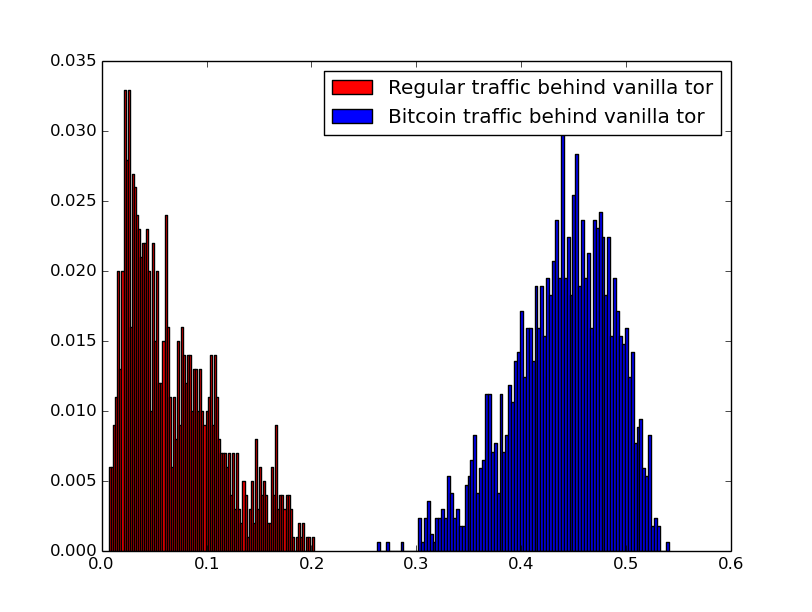
\includegraphics[width=\linewidth]{image/ratio_609_upstream_compact_vanilla_tor.png}
\caption{upstream}
\label{fig:ratio_609_upstream_compact_vanilla_tor}
\end{subfigure}
\begin{subfigure}{0.48\linewidth}
\centering
\includegraphics[width=\linewidth]{image/ratio_609_downstream_compact_vanilla_tor.eps}
\caption{downstream}
\label{fig:ratio_609_downstream_compact_vanilla_tor}
\end{subfigure}
\caption{Histogram of one cell packet ratio for HTTP traffic and \bc traffic}
\end{figure}
\bc traffic has a larger ratio of one-cell packets compared to Tor. This is due to a large number of small \bc messages (e.g., \code{inv}) that are each put into a single-cell packets. Figures \ref{fig:ratio_609_upstream_compact_vanilla_tor} and \ref{fig:ratio_609_downstream_compact_vanilla_tor} show the histogram of one cell size packets ratio in the upstream and downstream directions.

%As it is shown in Appendix~\ref{sec:charachterzing_bc}, the distribution of packet sizes differs in \bc and other types of traffic. While Tor modifies the sizes of \bc traffic, it does not remove all traffic patterns that reveal \bc. 

\iffalse, we show that this does not remove all traffic patterns that reveal \bc. We compare the distribution of packet sizes in HTTP traffic and \bc traffic behind Tor. 
Figures~\ref{fig:tor_reg_traffic_pkt_size_upstream} to \ref{fig:tor_compact_block_pkt_size_downstream} in Appendix~\ref{sec:bcshape} compare the distribution of packet sizes of HTTP and \bc when tunneled over Tor in different modes, showing an identifiable pattern.\fi
 
\subsection{Evaluating \bc over Tor}
\paragraphb{\code{SizeTor} classifier}
We implement ~\code{SizeTor} classifier on noisy \bc on compact mode for Tor and its three pluggable transports. As it is displayed in Figure~\ref{fig:tor_sizeTor}, we could detect \bc traffic with high accuracy for the complex user model when the background noise is one open tab. As Figure~\ref{fig:tor_sizeTor} indicates, having a traffic size of $10$ minutes is
enough to detect \bc traffic with around $90\%$ true positive and $0\%$ of false positive. Moreover, the Figure states that the result of classifier quickly diminishes when we increase the background noise from one to $2$ or $3$ open tabs.
Note that this figure shows the average result of this classifier on Tor and three pluggable transports.

\paragraphb{Neural Network-based classifier}
Table~\ref{tab:nn_tor} presents the result of NN-based classifier for the complex web user over Tor for $10,000$ numbers of test data. As the table suggests, performance of our classifier improves when we increase the size of training data. More specifically, our false positives enhances from $11\%$ to $4\%$ when we increase the training data from $1000$ to $40,000$. Moreover, when using $40,000$ training data, we reach $99\%$ and $4\%$ true and false positive, respectively ($97\%$ accuracy). Note that the reason we get better results from this classifier on Tor dataset is that this dataset only contains the complex web user since we did not have CAIDA application over Tor to use for our evaluation.
\begin{comment}
\begin{table}[h!]
  \begin{center}
     \caption{Result of Neural Network classifier for Tor dataset}
    \label{tab:nn_tor}
    \begin{tabular}{c|c|c|c}
    \kern 0.5pc \shortstack{ Training \\Size}& \shortstack{False Positive\\ ($\%$)} &\shortstack{True Positive\\ ($\%$)}&\shortstack{Accuracy \\($\%$)} \kern 0.5pc\\
      \hline
	$1000$&$11$ &$98 $  & $93$\\
	$5000$&$6$& $98$  & $96$\\
	$10,000$&$3$& $98$  &$ 97$\\
	$40,000$&$4$& $99$   & $97$\\
    \end{tabular}
  \end{center}
\end{table}
\end{comment}
\begin{table}
\center \caption{Result of neural network classifier on Tor dataset.}\label{tab:nn_tor}
\begin{tabular}{|c|c|c|c|}
\hline
 Training size& False positive ($\%$) &True positive ($\%$)&Accuracy ($\%$)\\
      \hline
	$1000$&$11$ &$98 $  & $93$\\
	$5000$&$6$& $98$  & $96$\\
	$10,000$&$3$& $98$  &$ 97$\\
	$40,000$&$4$& $99$   & $97$\\
\hline
\end{tabular}
\end{table}


\begin{figure}
\centering
\includegraphics[scale=0.15]{image/jan25/sizeTor-multiTab.pdf}%roc is also available
\caption{Detecting Bitcoin compact mode traffic behind Tor (Tor and its three pluggable transports: meek, obfs, fte) using SizeTor}
\label{fig:tor_sizeTor}
\end{figure}


\iffalse
\subsection{Bitcoin over VPN}
Another countermeasure that we evaluate is passing our traffic through VPN. Since VPN encrypts the traffic and 
\subsubsection{Evaluating Bitcoin over VPN}


\begin{figure*}[!t]
\begin{subfigure}{.48\linewidth}
\centering
\includegraphics[width=\linewidth]{image/jan25/vpn_d2u.pdf}
\caption{Result of \code{D2U} classifier according to traffic length and think time}
\label{fig:tp}
\end{subfigure}
\centering
\begin{subfigure}{.48\linewidth}
\includegraphics[width=\linewidth]{image/jan25/roc_vpn_d2u.pdf}
\caption{ROC curve for Think Time $=2$ minutes}
\label{fig:fp}
\end{subfigure}
\caption{Result of \code{D2U} classifier on \bc Traffic Tunneled over VPN}
\label{fig:vpn}
\end{figure*}
\fi





\paragraphb{Combined classifier over Tor}
We apply the combined classifier on our Tor dataset, which consists of \bc traffic with up to $5$ number of open tabs on the background. Our experiments show that having $40,000$ of training data is enough to achieve more than $99.72\%$ accuracy with $0.04\%$ false positive and $99.5\%$ true positive. Our combined classifier outperforms the previous classifiers (SizeTor and NN-based) on the Tor dataset as well. This is because we are using a more complex model and a more significant number of features.


\begin{comment}
\begin{table}
\center \caption{Result of combined classifier over Tor.}\label{tab:comb_t}
\begin{tabular}{|c|c|c|c|}
\hline
 Training size& False positive ($\%$) &True positive ($\%$)&Accuracy ($\%$)\\
      \hline
    $1000$    &$0.22$   & $71.36$   & $83.95$\\% for 50 epochs

	$5000$    &$0.79$   & $99.91$   & $99.6$\\% for 50 epochs
	$10,000$  &$0.0$   & $99.91$   & $99.95$\\% for 50 epochs
	$20,000$  &$0.0$  & $99.76$   & $99.84$\\% for 50 epochs
\hline
\end{tabular}
\end{table}

\end{comment}






%Figure~\ref{fig:d2u-Tor} shows the performance of our \code{D2U} classifier for the three transports, showing that it can reliably distinguish \bc traffic when there is HTTP browsing noise on the background. As it is shown from the figure, we are able to distinguish the \bc traffic with good accuracy in presence of background noise. 

\begin{comment}

Furthermore, We implement the D2U and SizeHist classifier on \bc traffic tunneled over Tor (Tor and three pluggable transports).
Figure~\ref{fig:tor_d2u} shows the result of the \code{D2U} classifier on \bc traffic (in compact block mode) tunneled over Tor.
Figure~\ref{fig:plug_tor_dow_up_ratio} shows the histogram of downstream-to-upstream traffic for \bc and HTTP using the three pluggable transports (no background noise). As can be seen, in the absence of the background noise there is a wide gap between the histograms of \bc and HTTP, allowing us to use the \code{D2U} classifier. Thus, we implemented \code{D2U} classifier for \bc traffic tunneled over three Tor pluggable transports. Figure~\ref{fig:tor_d2u} shows the average of result of this classifier for Tor and its three pluggable transports. The figure indicates that we can detect \bc traffic in presence of normal background noise with more than $0.80$ percent accuracy when we have $10$ minutes of \bc traffic and we can reach perfect accuracy when we increase the traffic length to $30$ minutes.


\begin{figure*}
\begin{subfigure}{0.32\linewidth}
\centering
\includegraphics[width=\linewidth]{image/obfs4_corr_value_btc_http.eps}
\caption{Obfs4}
\label{fig:obfs4_corr_value_btc_http}
\end{subfigure}
\begin{subfigure}{0.32\linewidth}
\centering
\includegraphics[width=\linewidth]{image/fte_corr_value_btc_http.eps}
\caption{FTE}
\label{fig:fte_corr_value_btc_http}
\end{subfigure}
\begin{subfigure}{0.32\linewidth}
\centering
\includegraphics[width=\linewidth]{image/meek_corr_value_btc_http.eps}
\caption{Meek}
\label{fig:meek_corr_value_btc_http}
\end{subfigure}
\caption{Histogram of downstream to upstream ratio for 30 minutes of traffic}
\label{fig:plug_tor_dow_up_ratio}
\end{figure*} 
\end{comment}

\begin{comment}
\begin{figure*}
\begin{subfigure}{0.32\linewidth}
\centering
\includegraphics[width=\linewidth]{image/jan25/tor_all_sizetor.pdf}
\caption{SizeTor}
\label{fig:tor_sizeTor}
\end{subfigure}
\begin{subfigure}{0.32\linewidth}
\centering
\includegraphics[width=\linewidth]{image/jan25/tor_all_d2u.pdf}
\caption{D2U}
\label{fig:tor_d2u}
\end{subfigure}
\begin{subfigure}{0.32\linewidth}
\centering
\includegraphics[width=\linewidth]{image/jan25/tor_all_sizehist.pdf}
\caption{SizeHist}
\label{fig:sizeHist}
\end{subfigure}
\caption{Detecting Bitcoin traffic behind Tor (Tor and its three pluggable transports: meek, obfs, fte) Using different classifiers}
\label{fig:vanilla_tor_effect_users}
\end{figure*} 
\end{comment}
\begin{comment}
In section~\ref{sec:exp}, we showed that our classifiers are able to detect \bc traffic with good accuracy.
As we noted before, some of our classifiers won't be able to detect \bc traffic when we add some cover traffic. But some of the classifiers resist in presence of large noise (neural net on Volume per sec). Here, we want to find possible countermeasures which would resist our classifiers.

Another possible countermeasure is to add some cover traffic to hide \bc traffic. We need to add as much traffic which is enough to dominates \bc traffic and thus, hide it. But at the same time, we do not want to add an enormous amount of traffic to have a high overhead. 
 The question that arises here is that: how much cover traffic do we need to hide \bc traffic. To find the minimum of cover traffic which hides \bc traffic, we do experiment with different amount of browsing traffic. 
\end{comment}


\section{Related Work}\label{related}
\red{i spotted some formatting/ grammar issues. please proofread.}

\red{shrink related work to make room for important text you removed. this is too long. }

In this section, we overview previous work on 
classifying different protocols and discuss previous attacks on \bc cryptocurrency.

\subsection{Protocol Classification}
There is extensive work in literature attempting to classify different applications or protocols in the network. Previously, researchers were focused on classification according to the port numbers~\cite{tcp_p2p,ports,port_mad,payload_p2p} and payload~\cite{payload_p2p,payload_content,payload_app,payload_moore}. Since many applications use uncertain port numbers~\cite{ports}, or some encrypt their payloads, researchers adopted new methods for protocol classification.
Recent techniques use statistics such as packet sizes and timings for classification~\cite{real_enc,web_p2p,blinc,prot_fing,semi,trafficClassSVM,svm2}. 

In some of the studies, researchers apply machine learning techniques on these statistics to classify different applications.%\cite{semi, svm2,MooreZ05,mlEffi}.
For example, in~\cite{semi}, authors take a semi-supervised approach to classify a variety of applications such as FTP, HTTP, P2P.  
In~\cite{trafficClassSVM,svm2}, authors use SVM classifier to distinguish different applications such as WWW, Mail, and FTP. Also, in~\cite{svm2}, authors use SVM to classify a broad application category such as mail, buck traffic, service. Moreover, in~\cite{survey_ml,myth}, authors survey the papers on Internet traffic classification using machine learning techniques.
\begin{comment}
In~\cite{MooreZ05}, Andrew W. Moore et al. use two refinements on the Bayesian technique and show that they can reach $95\%$ of accuracy on Internet traffic classification. Moreover, in~\cite{bays2}, authors use the Bayesian neural network to classify Internet traffic using just header-derived statistics. 
 In ~\cite{mlEffi}, Wei Li et al. use C4.5~\cite{tree} decision tree to classify Internet traffic such as mail, gaming, database, and browsing. They reach an accuracy of $99.8$, using $12$ features collected at the start of the flow.
   \end{comment}
 
 

  \subsection{Attacks on \bc Cryptocurrency}
 In this section, we discuss the previous attacks on the \bc network. 
 In~\cite{hijack}, the authors discuss routing attacks, their impact, and possible countermeasures. They study partitioning and delay attacks by investigating node-level and network-wide attacks for both. 
In~\cite{eclipse}, authors design eclipse attack in which the attacker isolate a victim from its peers by monopolizing its all incoming and outgoing connections, and filters her view of the network. In doing so, the attacker wastes her computing power on an outdated view of the network.

In~\cite{analysis_anon,privacy_anon}, authors use \bc transaction patterns
to link users (or link transactions) using some side information.
In~\cite{deanom1}, the authors propose a technique to link the public key of a user to her address or link her transactions. They show that they could launch their attacks even when the clients are behind NAT using only a few machines.
 In~\cite{double}, they analyze the security of using \bc for fast payments and show that the current \bc system is not secure unless they integrate \bc network with some detection mechanism.
 Also, they study double-spending attacks on fast payments and implement a method to prevent it.
 In~\cite{majority}, the authors introduce selfish-mine in which a pool can obtain a revenue larger than its share of mining power by forcing the honest miners to work on the wrong block, and therefore, waste their computing power.
%In~\cite{refund}, the authors propose a new attack on the \bc payment system that exploits some authentication vulnerability, or some weakness on the refund procedure. They suggest a revision on the \bc payment protocol, which prevents both attacks.

\section{Conclusions}

The reliable access to \bc and similar cryptocurrencies is of crucial importance due to
their consumers and the related industry. 
In this paper, we investigated the resilience of \bc to blocking by a powerful network entity such as an ISP or a government.
By characterizing \bc's communication patterns, we designed 
various classifiers that could distinguish (and therefore block) \bc traffic 
even if it is tunneled over an encrypted channel like Tor, 
and even when it is mixed with background traffic. Through extensive experiments on network traffic, we demonstrated that our classifiers could reliably identify \bc traffic despite using obfuscation protocols like Tor pluggable transports that modify traffic patterns. In order to disguise such patterns, an obfuscating protocol needs to apply significant cover traffic or employ large perturbations, which is undesirable for typical clients. 
%We suggest that future work should look into designing obfuscation protocols that are tailored to \bc (and similar cryptocurrencies) in a way to optimize resilience to detection and resource efficiency

%We learn from our experiments that it is
%extremely hard to hide Bitcoin traffic using standard obfuscation mechanism due to specific protocol messages with unique sizes and frequencies. . 
 
\section*{Acknowledgements}
The work was supported by the NSF CAREER grant CNS-1553301.




%% The next two lines define the bibliography style to be used, and
%% the bibliography file.
\bibliographystyle{abbrv}
%\bibliographystyle{plain}
\bibliography{refs, censBib}

%%
%% If your work has an appendix, this is the place to put it.
%\appendix


%\section{Background on \bc and Its Network Traffic}\label{sec:back}


\bc is the most popular cryptocurrency. It uses  a decentralized, peer-to-peer architecture~\cite{nakamoto2008bitcoin}, where each peer (e.g., client) is identified by her unique public key.  
	\bc clients exchange money through \bc transactions, which are  broadcasted on \bc's p2p network. 

	To prevent double spending and similar violations, \bc uses a public ledger called the \emph{blockchain} to store all \bc transactions. The blockchain is a chain of \emph{blocks}, where  each block contains a set of transactions and a \textit{proof-of-work}. A proof-of-work is a piece of data which is time-consuming and costly to generate. However, verifying the proof-of-work is easy. Each block is valid if and only if all of its transactions and its proof-of-work are valid. A verified block is broadcast on the network to update all peers' local ledgers. 
\begin{comment}	
\paragraphb{\bc's P2P Network.}
	\bc nodes form a full-mesh P2P network, and they connect to each other over unencrypted TCP connections. 
	Each node can connect to up to 125 peers, where up to 8 of them are  outgoing connections and the rest are incoming connections. A node stays connected to a neighbor until they restart or drop, in which case the node tries to replace them~\cite{Bitcoinnetworkoverview}. 
	%Since connection is without authentication, peers just keep a list of their connection IP addresses.
	Blocks and transactions are propagated by gossip. To avoid DoS attacks, peers only forward valid blocks and transactions; invalid blocks are discarded. 
	\end{comment}
%Bitcoin peers can be separated into two types: routable and non-routable. The former are capable of accepting incoming connections, and the latter are not, for example because they are behind a NAT or firewall.% However, it is worth mentioning that the official {\tt Bitcoind} software does not precisely split its functionality among routable and non-routable peers. 

\paragraphb{\bc Protocol Messages.}
	 \bc communications involve various protocol messages that are created by \bc peers. 
	 We divide \bc protocol messages into two classes: \emph{synchronization messages},  which are used for  propagating user addresses and transactions in the \bc network, and \emph{block-related messages}.%, which are responsible for disseminating \bc blocks. We introduce  major \bc messages in  Table~\ref{tab:bc-proto-list}.
	
%\section{Characterizing \bc Traffic}\label{sec:char}
\subsection{Synchronization Messages}
These messages are aimed at keeping \bc peers synchronized with the rest of the \bc network. %These messages are as following: \textbf{addr}, \textbf{inventory(inv)},\textbf{getdata}, and \textbf{tx}.

\code{\textbf{addr:}}Each peer advertises the information and IP addresses of other peers via \code{\textbf{addr}} message in the network. %\code{addr} message contains count and list of other peers IP addresses. Each IP address is accompanied by a timestamp showing its freshness. When a peer receives a list of addresses from other peers, it has a choice to forward any number of them. The peer chooses the sending addresses based on the following criteria: 1)~The number of IP addresses in the received message should not be greater than 10,and 2)~The timestamps should not be older than 10 minutes. This mechanism is applied for helping in peer discovery. 

\code{\textbf{inventory(inv):}} Peers send \code{inv} to advertise their knowledge about the known objects, like transactions and blocks.% Each \code{inv} message consist of number of inventory entries and the inventory vectors itself.% It can be received unsolicited, or in reply to \code{getblocks}.
%Inventory vectors  are used for notifying other nodes about objects they have or data which is being requested. Inventory vectors consist of the type of objects and the hash of the object. 

\code{\textbf{getdata:}} A peer sends \code{getdata} message in response to the \code{inv} to retrieve information about the content of an object, which can be a block or a transaction. 

\code{\textbf{tx}:} This message describes a transaction in response to a \code{getdata} message.% Each transaction is stored in a memory pool. If a received transaction is already in the pool, or it is included in one of the blocks in the main block-chain, it get discarded. 

% then the receiving peer runs several checks on the transaction's advertisement. If the checks passed, then the receiving peer asks for the transactions.

\subsection{Block-Related Messages} Such messages are used to exchange \bc blocks among the peers. 
The current \bc network is supporting two ways of propagating blocks, full block and compact block
propagation. %Figure~\ref{fig:protocol-flow} demonstrates the flow of message communication in these
%two ways.

\begin{comment}
  \begin{figure}[h]
\centering
\includegraphics[scale=0.45]{image/btc-protocol-flow.pdf}
\caption{Different relaying modes in  Bitcoin}
\label{fig:protocol-flow}
\end{figure}
\end{comment}

\paragraphe{Full Block Propagation:} The sender node first validate the block completely, then it advertise the possession of block by \code{inv} message. The receiving peer which doesn't have the block, asks for it by sending \code{getdata} message. Finally, the sender node send the block via \code{block} message. Sending full block in the network is wasting network bandwidth since we are re-sending all of the transaction and nodes have some of transaction in their memory pool. The messages transmitted in this mode is: 

\code{\textbf{block:}} It consist of block version information, previous block hash, merkle root of a Merkle tree collection which is a hash of all transactions related to this block. Sending  the new block forwarded through all the network.

%\amir{the two parts are uneven regarding how much you discuss}
\paragraphe{Compact Block Propagation:}
From the middle of 2016 in \code{0.13.0} version, Bitcoin protocol start to forward blocks as compact blocks which means instead of forwarding full blocks in network, only a sketch of block is sent. The sketch include 80-byte block's header, the short transactions IDs used for matching already-available transactions and select of transactions which sending peer expect that a receiving peer may be missing.% After receiving the compact block, the receiving peer tries to reconstruct the block at its end, from the already received transactions and the one in compact block. In this way the waste of sending each transaction twice is reduced. The advantage of compact block relaying is reducing the spikes in the bandwidth and  also reduce propagation delay. The messages transmitted in this mode are: 

\code{\textbf{sendcmpct:}} This message informs the receiving peer about the mode of communication the sending peer has chosen (low or high bandwidth). %If the first byte of the message is set to 1 the sender is indicating that it wants to receive blocks as soon as possible and it is working in the high-bandwidth mode. If the first byte of the message is set 0 the sender is saying that it wants to minimize bandwidth usage as much as possible and it is working in the low-bandwidth mode.

\code{\textbf{cmpctblock}:} This message introduced in the compact block relaying and is presenting a sketch of block.

\code{\textbf{getblocktxn}:} This message is introduced in compact block relaying and is used to request for the transactions that are missed by sending a list of their indexes. 

\code{\textbf{blocktxn}:} This message is introduced in compact-block relaying and is used to provide some of the transactions in a block, as requested.

\begin{comment}
Compact block relaying works in high and low bandwidth settings. In high bandwidth the receiving peer doesn't oblige the sending peers to ask for permission first. So, multiple peers can send the compact block to receiving node. Then at last the sender node sends the missing transactions by \code{blocktxn} message. It is worth mentioning \bc works in high bandwidth mode with up to 3 peers. 
However, in low bandwidth mode, since bandwidth is its bottleneck, the receiving node oblige other nodes to ask for permission first. So, the sender first advertise the block possession by \code{inv} message. Then, the receiving node asks for the compact block by \code{getdata} and the sender will send the compact block by \code{cmpctblock} message. At last, if there is any missing transaction, the receiving node will ask for it by \code{getblocktxn} and the sender will send those transactions via \code{blocktxn}. 
\end{comment}
\begin{comment}


\begin{table*}[!h]
\caption{The list of Bitcoin communication messages}\label{tab:bc-proto-list}
\centering
\begin{tabular}{| c | l |} \hline
Message & Description \\ \hline
\code{version}
& \shortstack{Advertise the node's version. No further communication is possible until \\both peers have exchanged their version.}  \\ \hline
\code{verack}
& Reply to the \code{version} message. \\ \hline
\code{addr}
& Send information about the known nodes of the network. \\ \hline
\code{inv}
& \shortstack{Sent to advertise the knowledge of the peer about the known objects. It can be received unsolicited, \\or in reply to \code{getblocks}.} \\ \hline
\code{getdata}
& Sent in response to the \code{inv} message to retrieve information about the content of an object. \\ \hline
\code{notfound} & If the receiver of \code{getdata} cannot return the requested information, it respond with \code{notfound} \\ \hline
\code{getblocks} & It return an \code{inv} message with the list of block after the specified block in \code{getblocks} request \\ \hline
\code{getheaders} & It return a \code{headers} message with the list of block after the specified block in \code{getblocks} request \\ \hline
\code{tx} 
& Sent to describes a Bitcoin transaction in response to a 
\code{getdata} message. \\  \hline
\code{block} &  \code{block} message is sent in response to a \code{getdata} message \\ \hline
\code{headers} &  Return a list of block headers, in respond to \code{getheaders} \\ \hline
\code{getaddr} & A node sends \code{getaddr} to ask about the known peer  from other peers  \\ \hline
\code{mempool} & It asks about the transaction in mempool of other peers \\ \hline
\code{ping}
& Show the TCP/IP connection is still valid. \\ \hline
\code{pong}
& Response to \code{ping} message. \\ \hline
\code{reject} & It show a message has been rejected \\ \hline
\code{sendheaders} & let other peers to send headers without \code{inv} message \\ \hline
\code{sendcmpct} &  let other peers to send compact blocks   \\ \hline
\code{cmpctblock} & it used in stead of \code{block}, to send cmpctblock \\ \hline
\code{getblocktxn} & it indicate missing block in compact block transaction \\ \hline
\code{blocktxn} & To send missing block in compact block transaction \\ \hline
\end{tabular}
\label{table:msg_description}
\end{table*}
\end{comment}


\begin{comment}
\section{Distribution of Packet Sizes over Tor}\label{sec:bcshape}

Figure~\ref{fig:tor_reg_traffic_pkt_size_upstream}-\ref{fig:tor_fullblock_pkt_size_downstream} shows the upstream and downstream packet distribution of HTTP and \bc traffic behind Tor.
\begin{figure}[t]
\begin{subfigure}{0.48\linewidth}
\centering
\includegraphics[width=\linewidth]{image/tor_reg_traffic_pkt_size_upstream.eps}
\caption{HTTP, upstream}
\label{fig:tor_reg_traffic_pkt_size_upstream}
\end{subfigure}
\begin{subfigure}{0.48\linewidth}
\centering
\includegraphics[width=\linewidth]{image/tor_reg_traffic_pkt_size_downstream.eps}
\caption{HTTP, downstream}
\label{fig:tor_reg_traffic_pkt_size_downstream}
\end{subfigure} 
\begin{subfigure}{0.48\linewidth}
\centering
\includegraphics[width=\linewidth]{image/tor_compact_block_pkt_size_upstream.eps}
\caption{Bitcoin, Compact block, upstream}
\label{fig:tor_compact_block_pkt_size_upstream}
\end{subfigure}
\begin{subfigure}{0.48\linewidth}
\centering
\includegraphics[width=\linewidth]{image/tor_compact_block_pkt_size_downstream.eps}
\caption{Bitcoin, Compact block, downstream}
\label{fig:tor_compact_block_pkt_size_downstream}
\end{subfigure} 
\begin{subfigure}{0.48\linewidth}
\centering
\includegraphics[width=\linewidth]{image/tor_fullblock_pkt_size_upstream.eps}
\caption{Bitcoin, Full block, upstream}
\label{fig:tor_fullblock_pkt_size_upstream}
\end{subfigure}
\begin{subfigure}{0.48\linewidth}
\centering
\includegraphics[width=\linewidth]{image/tor_fullblock_pkt_size_downstream.eps}
\caption{Bitcoin, Full block, downstream}
\label{fig:tor_fullblock_pkt_size_downstream}
\end{subfigure}
\caption{Distribution of packet sizes of HTTP and Bitcoin traffic behind Tor}
\end{figure}
\end{comment}
%\section{Algorithm for Window-based classifier}

\section{Threat Model}



\fatemeh{we did not have any text in  here}
\red{this section is so bad. it is not about threat model and it is too short. please put back the previous text that we had so i edit. }


 






\end{document}
